%% Generado por html2tex.py desde temas.json (qui). No editar a mano: corregir la clase en el .js del sitio y regenerar.
\parteciencia{qui}
\chapter{Estructura atómica}
%% =====================================================================
%% qui_mezclas
\section[Sustancias puras y mezclas]{Sustancias puras y mezclas}
\modcomun\ \ {\color{gris}\itshape Cómo se clasifica la materia (elementos, compuestos, mezclas homogéneas y heterogéneas) y cómo se separan las mezclas por filtración, tamizado, decantación y destilación, con sus aplicaciones.\par}
\subsection{Cómo se clasifica la materia}
Todo lo que tiene masa y ocupa espacio es \textbf{materia}. Para ordenarla, la química se hace una primera pregunta: ¿está formada por \textbf{una sola sustancia} o por \textbf{varias}?

 

\textbf{Sustancia pura.} Tiene composición fija y propiedades constantes: siempre funde y hierve a la misma temperatura (a igual presión). Hay dos tipos:

 
\begin{itemize}
  \item \textbf{Elemento:} formado por un solo tipo de átomo. Ejemplos: hierro (Fe), oxígeno (O\textsubscript{2}), helio (He).
  \item \textbf{Compuesto:} dos o más elementos unidos químicamente en una proporción fija. Ejemplos: agua (H\textsubscript{2}O), sal (NaCl), dióxido de carbono (CO\textsubscript{2}).
\end{itemize}
 

\textbf{Mezcla.} Dos o más sustancias juntas, sin reaccionar, en proporción variable. Cada una conserva sus propiedades y se pueden separar por \textbf{métodos físicos}. Hay dos tipos:

 
\begin{itemize}
  \item \textbf{Homogénea:} se ve uniforme, una sola fase. Ejemplos: agua con sal, aire, vinagre, bronce.
  \item \textbf{Heterogénea:} se distinguen dos o más fases. Ejemplos: agua con aceite, arena con agua, granito.
\end{itemize}
  
\begin{clave}[{Cómo leer un diagrama de partículas}] Cada color es un tipo de átomo. Mira cuántos \textbf{tipos de partículas} hay en el recuadro:\par · un solo tipo de partícula \ensuremath{\rightarrow} sustancia pura (si tiene un color, elemento; si tiene dos o más colores unidos, compuesto);\par · dos o más tipos de partículas \ensuremath{\rightarrow} mezcla.\end{clave}
  
\begin{center}
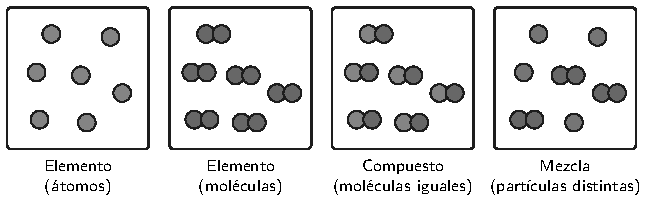
\includegraphics[max width=0.92\linewidth,max height=8.5cm]{qui/atomo_particulas}
\end{center}
\subsection{Elementos y compuestos}
Un \textbf{elemento} no se puede descomponer en sustancias más simples, ni siquiera con una reacción química. Hay cerca de 118, todos en la tabla periódica. Algunos están como átomos sueltos (He, Ne, Fe) y otros como moléculas de átomos iguales (O\textsubscript{2}, N\textsubscript{2}, Cl\textsubscript{2}, O\textsubscript{3}).

 

Un \textbf{compuesto} sí se puede descomponer, pero solo con una \textbf{reacción química}. Por ejemplo, al pasar corriente eléctrica por agua (electrólisis) se obtienen dos gases: hidrógeno y oxígeno.

 

Dos ideas importantes de los compuestos:

 
\begin{itemize}
  \item \textbf{Proporción fija:} el agua siempre tiene 1 g de hidrógeno por cada 8 g de oxígeno, venga de un río o de un glaciar.
  \item \textbf{Propiedades nuevas:} el sodio es un metal que reacciona violentamente con el agua y el cloro es un gas verde y tóxico; juntos forman la sal de mesa, NaCl, que comemos todos los días.
\end{itemize}
  
\begin{ejemplo}[{Ejemplo resuelto}] Clasifica: oro, aire, agua destilada, bronce, CO\textsubscript{2} y ozono (O\textsubscript{3}).\par · Oro (Au): un tipo de átomo \ensuremath{\rightarrow} \textbf{elemento}.\par · Ozono (O\textsubscript{3}): tres átomos, pero todos de oxígeno \ensuremath{\rightarrow} \textbf{elemento}.\par · Agua destilada (H\textsubscript{2}O) y CO\textsubscript{2}: dos elementos unidos \ensuremath{\rightarrow} \textbf{compuestos}.\par · Aire (N\textsubscript{2}, O\textsubscript{2}, Ar, CO\textsubscript{2}\dots{}) y bronce (cobre con estaño): varias sustancias, uniformes \ensuremath{\rightarrow} \textbf{mezclas homogéneas}.\end{ejemplo}
 
\begin{ojo}[{Error típico}] «El O\textsubscript{2} es un compuesto porque tiene dos átomos». No: para ser compuesto debe tener átomos de \textbf{elementos distintos}. Y el agua de la llave no es sustancia pura: lleva sales disueltas. La sustancia pura es el agua destilada.\end{ojo}
\subsection{Mezclas homogéneas y heterogéneas}
Una \textbf{fase} es una parte de la mezcla con el mismo aspecto y las mismas propiedades en todos sus puntos.

 
\begin{itemize}
  \item \textbf{Mezcla homogénea} (o solución): una sola fase. No distingues sus componentes ni con lupa: agua con azúcar, aire, vinagre, acero, bronce.
  \item \textbf{Mezcla heterogénea}: dos o más fases. Agua con aceite, arena con agua, granito, ensalada. La leche y la niebla (coloides) también se clasifican como heterogéneas: al microscopio se ven gotitas o partículas separadas.
\end{itemize}
 

\textbf{¿Por qué el agua y el aceite no se mezclan?} Por la regla «\textbf{lo semejante disuelve a lo semejante}»: las sustancias \textbf{polares} (agua, etanol, acetona) se mezclan entre sí y disuelven sales como el NaCl; las \textbf{apolares} (aceite, hexano, bencina) se mezclan entre sí. Un líquido polar con uno apolar forma dos fases: es una mezcla heterogénea.

  
\begin{clave}[{Esquema para clasificar}] 1. ¿Es uniforme en todos sus puntos? \textbf{No} \ensuremath{\rightarrow} mezcla heterogénea.\par 2. Si es uniforme: ¿se separa por procesos físicos (evaporar, destilar)? \textbf{Sí} \ensuremath{\rightarrow} mezcla homogénea.\par 3. Si no se separa por procesos físicos: ¿se descompone por procesos químicos? \textbf{Sí} \ensuremath{\rightarrow} compuesto. \textbf{No} \ensuremath{\rightarrow} elemento.\end{clave}
 
\begin{ejemplo}[{Ejemplo resuelto}] Al agregar sal a dos líquidos, se disuelve en el líquido T y queda en el fondo del líquido M. Entonces T se comporta como polar y M como apolar. Si se mezclan T y M, se formarán \textbf{dos fases}: una mezcla heterogénea.\end{ejemplo}
 
\begin{ojo}[{Ojo}] «Transparente» no significa «sustancia pura». El agua con sal es transparente y es una mezcla homogénea.\end{ojo}
\subsection{Separar mezclas: filtración y tamizado}
Como en una mezcla cada sustancia conserva sus propiedades, se separan aprovechando una \textbf{diferencia en alguna propiedad física}: tamaño de partícula, densidad, temperatura de ebullición o solubilidad.

 

\textbf{Filtración.} Separa un \textbf{sólido que no está disuelto} de un líquido. La mezcla pasa por un papel filtro: el sólido queda arriba (\textbf{residuo}) y el líquido pasa (\textbf{filtrado}). Se basa en el tamaño de las partículas. Ejemplos: colar el café, los filtros de agua, la mascarilla.

 

\textbf{Tamizado.} Separa \textbf{sólidos de distinto tamaño} con una malla o tamiz: los granos chicos pasan y los grandes quedan. Ejemplos: cernir harina, separar piedras de la arena en una construcción, clasificar mineral en la minería.

  
\begin{center}
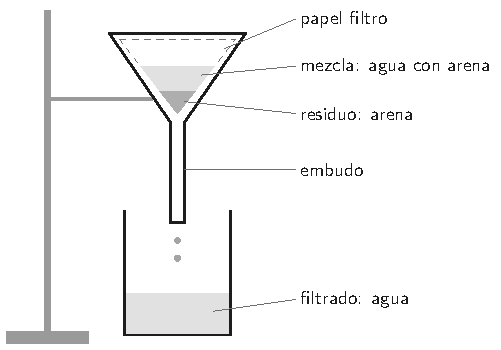
\includegraphics[max width=0.92\linewidth,max height=8.5cm]{qui/atomo_filtracion}
\end{center}
 
\begin{ojo}[{Error típico}] «Filtrando agua de mar obtengo agua sin sal». No: la sal está \textbf{disuelta}, sus partículas son tan pequeñas como las del agua y atraviesan el papel. Lo disuelto no se filtra.\end{ojo}
\subsection{Decantación}
La \textbf{decantación} separa componentes de \textbf{distinta densidad} que no se mezclan.

 

\textbf{Dos líquidos inmiscibles} (agua y aceite): se usa un \textbf{embudo de decantación}. Se deja reposar; el líquido más denso queda abajo. Se abre la llave, sale el líquido de abajo y se cierra justo cuando llega la línea que separa las fases.

 

\textbf{Sólido y líquido} (barro en agua): se deja reposar hasta que el sólido se va al fondo (sedimenta) y se vacía con cuidado el líquido de arriba.

 

\textbf{Aplicación: agua potable.} En las plantas de tratamiento se agregan \textbf{floculantes}, que juntan las partículas pequeñas en grumos (flóculos) más densos que el agua. Los flóculos se van al fondo (\textbf{decantación}) y lo que queda en suspensión se retiene con filtros de arena (\textbf{filtración}).

  
\begin{center}
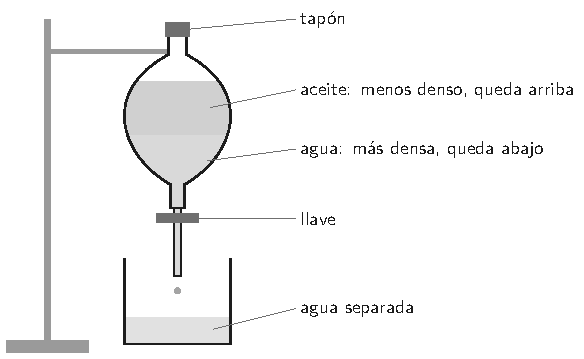
\includegraphics[max width=0.92\linewidth,max height=8.5cm]{qui/atomo_decantacion}
\end{center}
 
\begin{clave}[{Pariente cercano: la centrifugación}] Hace girar la mezcla muy rápido para que lo más denso se vaya al fondo en minutos. Así se separan el plasma y las células de la sangre.\end{clave}
\subsection{Destilación y evaporación}
\textbf{Destilación.} Separa un líquido de lo que tiene disuelto, o dos líquidos \textbf{miscibles} con distinta \textbf{temperatura de ebullición}. Se calienta la mezcla; el componente más volátil (menor temperatura de ebullición) se evapora primero, el vapor se enfría en el \textbf{refrigerante} y se recoge como líquido: el \textbf{destilado}.

 

La \textbf{destilación fraccionada} usa una columna para separar varios líquidos de temperaturas de ebullición cercanas. Así se separa el petróleo en gas, bencina, kerosene y diésel, y así se obtiene el pisco a partir del vino.

 

\textbf{Evaporación.} Si solo interesa el sólido disuelto, se evapora el líquido y el sólido queda. Así se obtiene la sal en las salinas de la costa y el litio en el Salar de Atacama.

  
\begin{clave}[{Mezclas de tres componentes}] Se separan por pasos, cada uno con su propiedad.\par · Arena + sal disuelta en agua: \textbf{filtrar} (queda la arena) y luego \textbf{evaporar} el filtrado (queda la sal).\par · Dos líquidos miscibles + un sólido insoluble: \textbf{filtrar} el sólido y luego \textbf{destilar} los líquidos.\end{clave}
  
\begin{center}
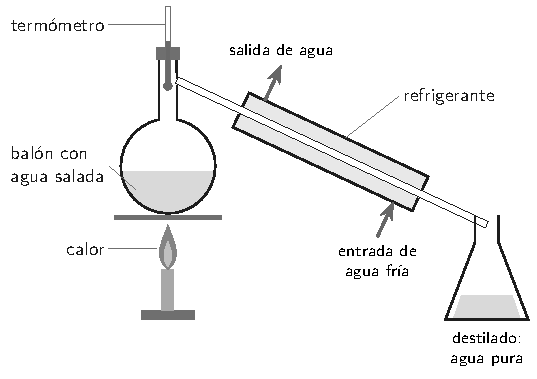
\includegraphics[max width=0.92\linewidth,max height=8.5cm]{qui/atomo_destilacion}
\end{center}
\subsection{Lo clave del tema}
\begin{center}\small
\begin{tabularx}{\linewidth}{@{}>{\raggedright\arraybackslash\hsize=0.51\hsize}X>{\raggedright\arraybackslash\hsize=1.45\hsize}X>{\raggedright\arraybackslash\hsize=0.91\hsize}X>{\raggedright\arraybackslash\hsize=1.13\hsize}X@{}}
\toprule
\textbf{Método} & \textbf{Qué separa} & \textbf{Propiedad que aprovecha} & \textbf{Ejemplo} \\
\midrule
Filtración & sólido no disuelto de un líquido & tamaño de partícula & arena del agua, café \\
Tamizado & sólidos de distinto tamaño & tamaño de partícula & piedras de la arena, harina \\
Decantación & líquidos inmiscibles, o sólido que sedimenta & densidad & agua y aceite, floculantes \\
Destilación & líquidos miscibles, o líquido de su soluto & temperatura de ebullición & petróleo, pisco, agua destilada \\
Evaporación & sólido disuelto de su solvente & volatilidad del solvente & sal de mar, litio \\
\bottomrule
\end{tabularx}
\end{center}
 
\begin{clave}[{Recuerda}] · O\textsubscript{2} es un elemento: todos sus átomos son iguales.\par · Un compuesto tiene partículas iguales formadas por átomos distintos; si hay dos tipos de partículas, es mezcla.\par · El agua con sal es transparente y es una mezcla homogénea.\par · La sal disuelta se separa evaporando o destilando.\par · Dos líquidos miscibles (una sola fase) se separan por destilación.\end{clave}
 
\begin{clave}[{Método PAES}] 1. Cuenta los tipos de partículas o de sustancias: uno \ensuremath{\rightarrow} sustancia pura; varios \ensuremath{\rightarrow} mezcla. 2. Pregunta si es uniforme (homogénea o heterogénea). 3. Para separar, identifica en qué se diferencian los componentes (tamaño, densidad, temperatura de ebullición) y elige el método que usa esa diferencia. 4. Si hay tres componentes, ordena los pasos: primero lo que no está disuelto, al final lo disuelto.\end{clave}
\begin{elejemplo}{PAES Invierno 2027, adaptada}
Un grupo de estudiantes recibe en el laboratorio una muestra de un material desconocido. Para clasificarlo, siguen una secuencia de preguntas y anotan las respuestas en el siguiente esquema:
\begin{center}
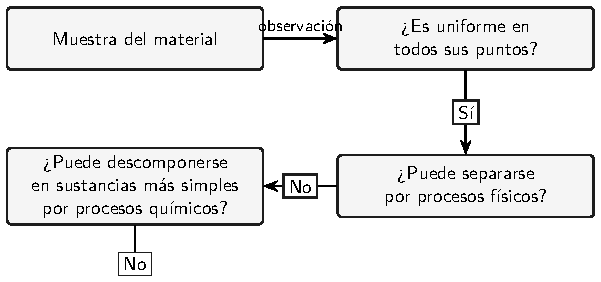
\includegraphics[max width=0.92\linewidth,max height=8.5cm]{qui/atomo_esquema}
\end{center}
\alts{A un elemento.}{A un compuesto.}{A una mezcla homogénea.}{A una mezcla heterogénea.}
\solucion{\textbf{Paso 1. ¿Qué nos piden?} Clasificar el material siguiendo las respuestas del esquema, una por una.

\textbf{Paso 2. ¿Es uniforme? Sí.} Tiene una sola fase. Queda descartada la mezcla heterogénea. Todavía puede ser mezcla homogénea, compuesto o elemento.

\textbf{Paso 3. ¿Se separa por procesos físicos? No.} Una mezcla homogénea, como el agua con sal, sí se separa por procesos físicos (evaporando el agua queda la sal). Como este material no se separa, no es mezcla: es una \textbf{sustancia pura}.

\textbf{Paso 4. ¿Se descompone por procesos químicos? No.} Un compuesto, como el agua, sí se descompone por una reacción química (la electrólisis la separa en hidrógeno y oxígeno). Como este material no se descompone en sustancias más simples, está formado por un solo tipo de átomo.

\textbf{Respuesta:} es un elemento.

\textbf{Comprobación:} un trozo de cobre cumple las tres respuestas: es uniforme, no se separa por filtración, destilación ni evaporación, y ninguna reacción lo convierte en sustancias más simples.

\textbf{¿Por qué no las otras?} «Compuesto» habría tenido «Sí» en la última pregunta: los compuestos se descomponen por procesos químicos. «Mezcla homogénea» habría tenido «Sí» en la segunda pregunta: las mezclas se separan por procesos físicos. «Mezcla heterogénea» habría tenido «No» en la primera: no es uniforme.

\textbf{\color{cienciaD}Para recordar.} Uniforme y sin separarse por métodos físicos es sustancia pura; si además no se descompone químicamente, es un elemento.}{A}
\end{elejemplo}

%% =====================================================================
%% qui_propiedades
\section[Propiedades físicas: densidad, fusión y ebullición]{Propiedades físicas: densidad, fusión y ebullición}
\modcomun\ \ {\color{gris}\itshape Masa, volumen y densidad (d = m/V), propiedades intensivas y extensivas, flotación y desplazamiento de agua; temperaturas de fusión y ebullición, estado físico de una sustancia y curvas de calentamiento de sustancias puras y mezclas.\par}
\subsection{Propiedades extensivas e intensivas}
Una \textbf{propiedad física} se puede medir sin cambiar la identidad de la sustancia: masa, volumen, densidad, temperatura de fusión, temperatura de ebullición, color.

 
\begin{itemize}
  \item \textbf{Extensivas:} dependen de \textbf{cuánta} materia hay. La \textbf{masa} (g, kg) y el \textbf{volumen} (mL, L, cm\textsuperscript{3}) son extensivas: un balde de agua tiene más masa y más volumen que un vaso.
  \item \textbf{Intensivas:} no dependen de la cantidad. La \textbf{densidad}, la \textbf{temperatura de fusión} y la \textbf{temperatura de ebullición} son intensivas: el agua de un vaso y la de un balde hierven a 100 °C a nivel del mar.
\end{itemize}
 

Las intensivas sirven para \textbf{identificar} una sustancia, porque son características de ella. Las extensivas no: 50 g puede ser de agua, de oro o de aire.

  
\begin{ejemplo}[{Ejemplo resuelto}] Un trozo de aluminio tiene 54 g y 20 cm\textsuperscript{3}. Se parte por la mitad. Cada mitad tiene 27 g y 10 cm\textsuperscript{3} (las extensivas se reducen a la mitad), pero la densidad sigue siendo $\dfrac{27}{10} = 2{,}7$ g/cm\textsuperscript{3} y la temperatura de fusión sigue siendo 660 °C (las intensivas no cambian).\end{ejemplo}
 
\begin{ojo}[{Cambio físico o químico}] En un cambio físico la sustancia sigue siendo la misma: el vapor que empaña un espejo sigue siendo agua. En un cambio químico se forma una sustancia nueva: el hierro que se oxida, la manzana que se pone café, el bicarbonato que burbujea con limón.\end{ojo}
\subsection{Densidad: d = m/V}
La \textbf{densidad} dice cuánta masa hay en cada unidad de volumen:

 \[ d = \dfrac{m}{V} \] 

Se mide en g/mL o g/cm\textsuperscript{3} (son lo mismo, porque 1 mL = 1 cm\textsuperscript{3}). El agua líquida tiene $d = 1$ g/mL: cada mililitro de agua tiene 1 g.

 

De la misma fórmula salen las otras dos:

 \[ m = d\cdot V \qquad\qquad V = \dfrac{m}{d} \] 

\textbf{Ejemplo 1.} Un bloque de plomo ($d = 11{,}3$ g/cm\textsuperscript{3}) tiene un volumen de 2,0 cm\textsuperscript{3}. Su masa es $m = 11{,}3\cdot 2{,}0 = 22{,}6$ g.

 

\textbf{Ejemplo 2.} ¿Qué volumen ocupan 46 g de etanol ($d = 0{,}8$ g/mL)? $V = \dfrac{46}{0{,}8} = 57{,}5$ mL.

  
\begin{center}\small
\begin{tabular}{@{}ll@{}}
\toprule
\textbf{Sustancia} & \textbf{Densidad (g/cm\textsuperscript{3})} \\
\midrule
aceite de cocina & 0,92 \\
hielo & 0,92 \\
agua líquida & 1,00 \\
aluminio & 2,7 \\
hierro & 7,9 \\
cobre & 8,96 \\
plomo & 11,3 \\
mercurio & 13,6 \\
oro & 19,3 \\
\bottomrule
\end{tabular}
\end{center}
 
\begin{ojo}[{Error típico}] Sumar o dividir al revés. Revisa las unidades: g/cm\textsuperscript{3} por cm\textsuperscript{3} da g (masa); g dividido por g/cm\textsuperscript{3} da cm\textsuperscript{3} (volumen). Si la unidad no calza, la operación está mal.\end{ojo}
\subsection{Medir el volumen: probeta y desplazamiento de agua}
La masa se mide con una \textbf{balanza}. El volumen de un líquido se mide con una \textbf{probeta}: se lee la marca que coincide con la parte baja de la curva del líquido (el menisco), con los ojos a la altura del líquido.

 

Un sólido de forma irregular, como una piedra, no se puede medir con regla. Se usa el \textbf{desplazamiento de agua}: al sumergirlo, el nivel sube exactamente lo que ocupa el sólido.

 

\textbf{Ejemplo resuelto.} Una piedra de 24 g se sumerge en una probeta con 20 mL de agua y el nivel sube a 28 mL.

 

\textbf{Paso 1.} Volumen de la piedra: $28 - 20 = 8$ mL $= 8$ cm\textsuperscript{3}.

 

\textbf{Paso 2.} Densidad: $d = \dfrac{24}{8} = 3$ g/cm\textsuperscript{3}.

  
\begin{center}
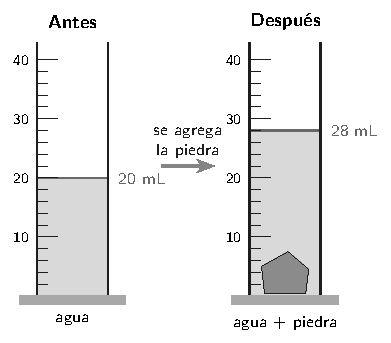
\includegraphics[max width=0.92\linewidth,max height=8.5cm]{qui/atomo_probeta}
\end{center}
 
\begin{ojo}[{Error típico}] Dividir por el volumen final (28 mL) o por el inicial (20 mL). El volumen del sólido es la \textbf{diferencia} entre las dos lecturas.\end{ojo}
 
\begin{clave}[{Precisión}] La probeta mide el volumen con menos precisión que la balanza mide la masa. Con volúmenes pequeños (1 o 2 mL), un error de lectura de 0,1 mL cambia mucho la densidad calculada.\end{clave}
\subsection{Flotación y gráficos de masa y volumen}
\textbf{Flotación.} Un objeto flota en un líquido si su densidad es \textbf{menor} que la del líquido, y se hunde si es mayor. Por eso el hielo (0,92 g/cm\textsuperscript{3}) flota en el agua y una moneda de cobre se hunde. Un huevo se hunde en agua, pero flota en agua con mucha sal: la sal disuelta aumenta la densidad del líquido.

 

Si se juntan líquidos que no se mezclan, se ordenan en capas: el más denso abajo y el menos denso arriba.

 

\textbf{Gráfico de masa versus volumen.} Para una sustancia, la masa es proporcional al volumen: el gráfico es una recta que pasa por el origen, y su \textbf{pendiente es la densidad}. Para leerla, elige un punto de la recta y divide masa por volumen. Mientras más inclinada la recta, mayor la densidad.

  
\begin{center}
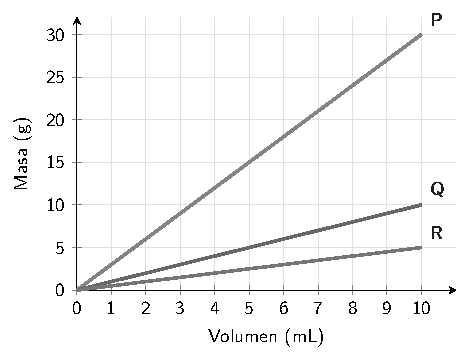
\includegraphics[max width=0.92\linewidth,max height=8.5cm]{qui/atomo_mv_1}
\end{center}
 
\begin{ejemplo}[{Ejemplo resuelto}] En el gráfico, P pasa por (10 mL, 30 g): $d = \dfrac{30}{10} = 3$ g/mL. Q pasa por (10 mL, 10 g): $d = 1$ g/mL, como el agua. R pasa por (10 mL, 5 g): $d = 0{,}5$ g/mL, así que R flota en agua y P se hunde.\end{ejemplo}
 
\begin{ojo}[{Ojo}] La densidad cambia con la temperatura: casi todas las sustancias se dilatan al calentarse, así que su densidad baja un poco. Por eso las tablas indican a qué temperatura se midió.\end{ojo}
\subsection{Temperaturas de fusión y ebullición}
\textbf{Temperatura de fusión:} a la que un sólido pasa a líquido (es la misma a la que el líquido se solidifica). Agua: 0 °C.

 

\textbf{Temperatura de ebullición:} a la que un líquido hierve y pasa a gas (es la misma a la que el gas se condensa). Agua: 100 °C a 1 atm. Depende de la presión: en la cordillera, con menos presión, el agua hierve a menos de 100 °C.

 

\textbf{¿En qué estado está una sustancia a una temperatura T?} Compara T con sus dos temperaturas:

 
\begin{itemize}
  \item T menor que la de fusión \ensuremath{\rightarrow} \textbf{sólido}.
  \item T entre la de fusión y la de ebullición \ensuremath{\rightarrow} \textbf{líquido}.
  \item T mayor que la de ebullición \ensuremath{\rightarrow} \textbf{gas}.
\end{itemize}
  
\begin{ejemplo}[{Ejemplo resuelto}] A 25 °C y 1 atm:
\begin{center}\small
\begin{tabular}{@{}llll@{}}
\toprule
\textbf{Elemento} & \textbf{Fusión (°C)} & \textbf{Ebullición (°C)} & \textbf{Estado} \\
\midrule
Cloro & \ensuremath{-}101 & \ensuremath{-}35 & gas (25 > \ensuremath{-}35) \\
Bromo & \ensuremath{-}7 & 59 & líquido (\ensuremath{-}7 < 25 < 59) \\
Yodo & 114 & 184 & sólido (25 < 114) \\
\bottomrule
\end{tabular}
\end{center}\end{ejemplo}
 
\begin{ojo}[{Error típico con negativos}] \ensuremath{-}35 °C es una temperatura \textbf{más baja} que 25 °C. Si la temperatura de ebullición es negativa, a temperatura ambiente la sustancia ya hirvió: es un gas.\end{ojo}
\subsection{Curvas de calentamiento}
Si se calienta una sustancia y se anota la temperatura cada minuto, se obtiene una \textbf{curva de calentamiento}.

 
\begin{itemize}
  \item En los tramos inclinados, la sustancia está en un solo estado y su temperatura sube.
  \item En los tramos horizontales (\textbf{mesetas}) ocurre un cambio de estado: la sustancia sigue recibiendo calor, pero esa energía se usa en separar las partículas y la temperatura no sube. La primera meseta es la \textbf{fusión} (sólido y líquido juntos) y la segunda, la \textbf{ebullición} (líquido y gas juntos).
\end{itemize}
 

\textbf{Sustancia pura o mezcla.} Una sustancia pura tiene mesetas planas: funde y hierve a una temperatura fija. Una mezcla funde y hierve en un \textbf{rango} de temperaturas: la «meseta» queda inclinada, porque la composición del líquido va cambiando mientras hierve.

  
\begin{center}
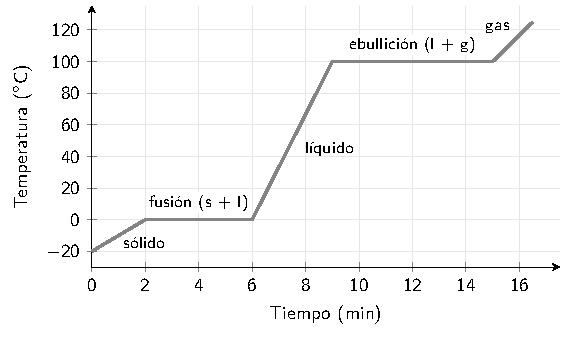
\includegraphics[max width=0.92\linewidth,max height=8.5cm]{qui/atomo_calentamiento}
\end{center}
 
\begin{center}
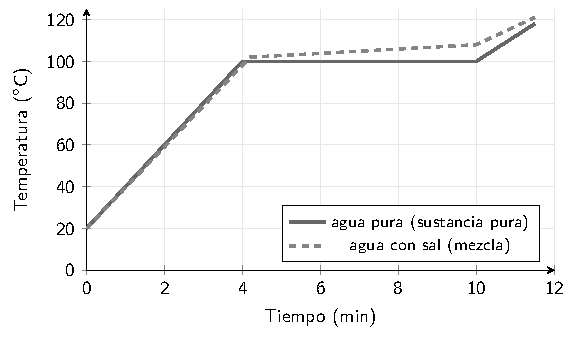
\includegraphics[max width=0.92\linewidth,max height=8.5cm]{qui/atomo_pura_mezcla}
\end{center}
\subsection{Lo clave del tema}
\begin{center}\small
\begin{tabularx}{\linewidth}{@{}>{\raggedright\arraybackslash\hsize=0.97\hsize}X>{\raggedright\arraybackslash\hsize=0.47\hsize}X>{\raggedright\arraybackslash\hsize=1.56\hsize}X@{}}
\toprule
\textbf{Propiedad} & \textbf{Tipo} & \textbf{Cómo se mide o calcula} \\
\midrule
Masa & extensiva & balanza (g) \\
Volumen & extensiva & probeta; sólidos irregulares, desplazamiento de agua (mL = cm\textsuperscript{3}) \\
Densidad & intensiva & $d = \dfrac{m}{V}$; pendiente del gráfico masa-volumen \\
Temperatura de fusión & intensiva & primera meseta de la curva de calentamiento \\
Temperatura de ebullición & intensiva & segunda meseta; depende de la presión \\
\bottomrule
\end{tabularx}
\end{center}
 
\begin{clave}[{Recuerda}] · La densidad es intensiva: si partes un objeto, no cambia.\par · $m = d\cdot V$ (revisa las unidades).\par · Volumen de la piedra = lectura final \ensuremath{-} lectura inicial.\par · En la meseta el calor que entra se usa en el cambio de estado.\par · Si una sustancia hierve a \ensuremath{-}35 °C, a 25 °C ya es gas.\end{clave}
 
\begin{clave}[{Método PAES}] 1. Anota los datos con sus unidades. 2. Elige la fórmula: $d = \dfrac{m}{V}$, $m = d\cdot V$ o $V = \dfrac{m}{d}$. 3. Revisa que las unidades den lo pedido. 4. Para el estado físico, ubica la temperatura entre la de fusión y la de ebullición. 5. En gráficos, lee primero los ejes y sus unidades; en tablas de datos, busca qué variable cambia junto con cuál.\end{clave}
\begin{elejemplo}{PAES Invierno 2027, adaptada}
Como parte de un proyecto escolar, un grupo de estudiantes midió la masa y el volumen de cinco muestras de cobre refinado, que la empresa minera etiqueta con una pureza de 99,99 \%. Con esos valores calcularon la densidad de cada muestra y la compararon con el valor de referencia del cobre, 8,96 g/cm\textsuperscript{3}. Todas las mediciones se hicieron con la misma balanza y la misma probeta, en una sala a temperatura constante:

La profesora les comenta que el trabajo tiene un problema de confiabilidad. ¿Cuál de los siguientes factores lo perjudicó?
\begin{center}\small
\begin{tabularx}{\linewidth}{@{}>{\raggedright\arraybackslash\hsize=0.57\hsize}X>{\raggedright\arraybackslash\hsize=0.51\hsize}X>{\raggedright\arraybackslash\hsize=1.37\hsize}X>{\raggedright\arraybackslash\hsize=1.54\hsize}X@{}}
\toprule
\textbf{Muestra} & \textbf{Masa (g)} & \textbf{Volumen (cm\textsuperscript{3})} & \textbf{Densidad (g/cm\textsuperscript{3})} \\
\midrule
\textbf{1} & 17,204 & 2,0 & 8,6 \\
\textbf{2} & 9,398 & 1,0 & 9,4 \\
\textbf{3} & 13,653 & 1,5 & 9,1 \\
\textbf{4} & 16,998 & 2,0 & 8,5 \\
\textbf{5} & 8,803 & 1,0 & 8,8 \\
\bottomrule
\end{tabularx}
\end{center}
\altslargas{La cantidad de muestras utilizadas.}{Los valores de volumen registrados.}{El uso de un valor de densidad de referencia.}{La procedencia de las muestras desde una empresa.}
\solucion{\textbf{Paso 1. ¿Qué nos piden?} Encontrar qué parte del trabajo hace que los resultados no sean confiables. Primero vemos si los datos tienen sentido.

\textbf{Paso 2. Revisa los cálculos.} $\dfrac{17{,}204}{2{,}0} = 8{,}6$; $\dfrac{9{,}398}{1{,}0} = 9{,}4$; $\dfrac{13{,}653}{1{,}5} = 9{,}1$; $\dfrac{16{,}998}{2{,}0} = 8{,}5$; $\dfrac{8{,}803}{1{,}0} = 8{,}8$. Las cuentas están bien hechas.

\textbf{Paso 3. ¿Qué esperábamos?} Las cinco muestras son del mismo cobre, casi puro. La densidad es intensiva: todas deberían dar casi lo mismo, cerca de 8,96 g/cm\textsuperscript{3}. Pero los resultados van de 8,5 a 9,4: varían demasiado.

\textbf{Paso 4. Busca la causa.} Las masas tienen tres decimales: la balanza es muy precisa. Los volúmenes tienen un solo decimal y son muy pequeños (1 o 2 cm\textsuperscript{3}), medidos con una probeta. Un error de lectura de solo 0,1 cm\textsuperscript{3} en 1,0 cm\textsuperscript{3} es un error del 10 \% en la densidad. Por ejemplo, la muestra 2 daría $\dfrac{9{,}398}{1{,}05} \approx 8{,}95$ g/cm\textsuperscript{3} si su volumen real fuera 1,05 cm\textsuperscript{3}, en vez de 1,0.

\textbf{Respuesta:} los valores de volumen registrados.

\textbf{Comprobación:} si el problema fuera la pureza, todas las densidades se correrían hacia el mismo lado; aquí unas quedan sobre 8,96 y otras bajo 8,96, que es lo típico de un error de medición al azar.

\textbf{¿Por qué no las otras?} Cinco muestras es una cantidad razonable; más muestras no arreglan una medición imprecisa. Comparar con un valor de referencia es justamente lo que permite detectar el problema. Que las muestras vengan de una empresa no afecta la medición: el cobre está etiquetado con 99,99 \% de pureza.

\textbf{\color{cienciaD}Para recordar.} Si una muestra pura da densidades muy distintas, revisa la precisión de las mediciones, sobre todo de los volúmenes pequeños.}{B}
\end{elejemplo}

%% =====================================================================
%% qui_modelos
\section[Modelos atómicos: de Dalton a Bohr]{Modelos atómicos: de Dalton a Bohr}
\modcomun\ \ {\color{gris}\itshape La teoría de Dalton y los modelos de Thomson, Rutherford y Bohr: qué propuso cada uno, qué experimento u observación lo motivó, qué explicó, cuáles fueron sus limitaciones y en qué orden aparecieron.\par}
\subsection{Por qué hay varios modelos atómicos}
Nadie ha visto un átomo a simple vista. Un \textbf{modelo atómico} es una representación que explica lo que se observa en los experimentos. Cuando aparece una observación que el modelo no puede explicar, se propone uno nuevo que sí la explique.

 

Así, cada modelo corrige al anterior:

 
\begin{center}\small
\begin{tabularx}{\linewidth}{@{}>{\raggedright\arraybackslash\hsize=0.72\hsize}X>{\raggedright\arraybackslash\hsize=0.81\hsize}X>{\raggedright\arraybackslash\hsize=1.48\hsize}X@{}}
\toprule
\textbf{Año} & \textbf{Modelo} & \textbf{Idea central} \\
\midrule
1808 & Dalton & átomos indivisibles \\
1897--1904 & Thomson & el átomo tiene electrones \\
1911 & Rutherford & núcleo pequeño, positivo y denso \\
1913 & Bohr & niveles de energía \\
1926 en adelante & mecano-cuántico & orbitales (zonas de probabilidad) \\
\bottomrule
\end{tabularx}
\end{center}
  
\gatotip[\gatogris]{\textbf{Para recordar el orden.} Cada modelo agrega algo «más adentro» del átomo: Dalton (el átomo entero) \ensuremath{\rightarrow} Thomson (sus electrones) \ensuremath{\rightarrow} Rutherford (su núcleo) \ensuremath{\rightarrow} Bohr (la energía de los electrones).}
  
\begin{center}
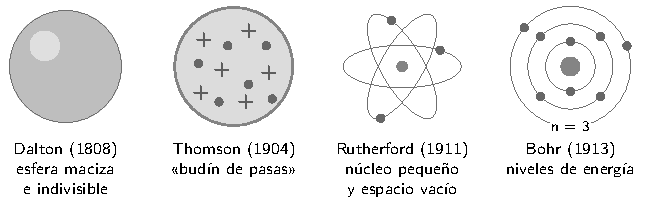
\includegraphics[max width=0.92\linewidth,max height=8.5cm]{qui/atomo_modelos}
\end{center}
\subsection{Dalton: el átomo indivisible}
John Dalton (1808) propuso la primera teoría atómica con base experimental. Sus postulados:

 
\begin{itemize}
  \item La materia está formada por partículas muy pequeñas e \textbf{indivisibles}: los átomos.
  \item Los átomos de un mismo elemento son \textbf{iguales} entre sí (misma masa y propiedades) y distintos de los de otros elementos.
  \item Los compuestos se forman al combinarse átomos de distintos elementos en \textbf{proporciones de números enteros sencillos}.
  \item En una reacción química los átomos \textbf{se reordenan}: no se crean ni se destruyen.
\end{itemize}
 

Con esto explicó la ley de conservación de la masa y la ley de las proporciones definidas.

  
\begin{ojo}[{Limitaciones}] El átomo \textbf{sí es divisible}: tiene electrones, protones y neutrones. Y no todos los átomos de un elemento tienen la misma masa: existen los \textbf{isótopos}. Su modelo no dice nada sobre cargas eléctricas.\end{ojo}
 
\begin{ejemplo}[{Ejemplo resuelto}] ¿Qué postulado de Dalton explica que en una reacción la masa total no cambie? El último: los átomos solo se reordenan. Si hay los mismos átomos antes y después, la masa es la misma.\end{ejemplo}
\subsection{Thomson: el descubrimiento del electrón}
J. J. Thomson trabajó con \textbf{tubos de rayos catódicos}: tubos de vidrio casi sin aire, con un metal en cada extremo conectado a alto voltaje. Desde el polo negativo salía un rayo que se desviaba hacia una placa con carga \textbf{positiva}.

 

\textbf{Conclusión:} el rayo está formado por partículas con \textbf{carga negativa}, mucho más livianas que un átomo, y aparecen con cualquier metal. Esas partículas, los \textbf{electrones}, forman parte de todos los átomos. Por lo tanto, el átomo \textbf{no es indivisible}.

 

\textbf{Modelo del «budín de pasas»} (1904): el átomo es una esfera con carga positiva repartida de manera uniforme, y los electrones están incrustados en ella, como pasas en un budín. Las cargas positivas y negativas se compensan: el átomo es neutro.

  
\begin{ojo}[{Limitación}] Con la carga positiva repartida por toda la esfera, ninguna partícula debería rebotar al chocar con un átomo. El experimento de Rutherford mostró lo contrario.\end{ojo}
 
\begin{clave}[{Error típico}] «Thomson descubrió el núcleo». No: Thomson descubrió el \textbf{electrón}. El núcleo lo propuso Rutherford.\end{clave}
\subsection{Rutherford: el experimento de la lámina de oro}
En 1911, el equipo de Ernest Rutherford bombardeó una lámina de oro muy delgada con \textbf{partículas alfa} (partículas con carga positiva) y registró hacia dónde salían en una pantalla.

 
\begin{center}\small
\begin{tabularx}{\linewidth}{@{}>{\raggedright\arraybackslash\hsize=1.00\hsize}X>{\raggedright\arraybackslash\hsize=1.00\hsize}X@{}}
\toprule
\textbf{Observación} & \textbf{Conclusión} \\
\midrule
Casi todas pasan sin desviarse & el átomo es casi todo \textbf{espacio vacío} \\
Algunas se desvían & hay una zona con carga \textbf{positiva} que las repele \\
Muy pocas (1 de cada 10.000 a 100.000) rebotan & esa zona es muy \textbf{pequeña} y muy \textbf{densa}: concentra casi toda la masa \\
\bottomrule
\end{tabularx}
\end{center}
 

\textbf{Modelo nuclear} (o planetario): un \textbf{núcleo} diminuto, positivo, con casi toda la masa del átomo, y los electrones girando alrededor, lejos de él. Si el átomo fuera un estadio, el núcleo sería una bolita en el centro de la cancha.

  
\begin{ojo}[{Limitación}] Según la física de la época, un electrón que gira debería emitir energía, perder velocidad y caer en espiral al núcleo: el átomo no sería estable. Tampoco explicaba por qué cada elemento emite luz solo de ciertos colores.\end{ojo}
  
\begin{center}
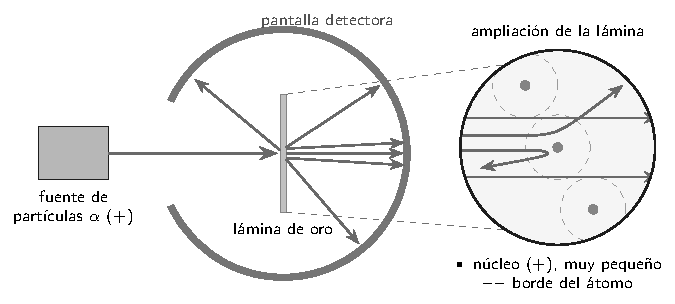
\includegraphics[max width=0.92\linewidth,max height=8.5cm]{qui/atomo_rutherford}
\end{center}
\subsection{Bohr: los niveles de energía}
Niels Bohr (1913) mantuvo el núcleo de Rutherford y agregó reglas para los electrones:

 
\begin{itemize}
  \item Los electrones giran en \textbf{órbitas circulares} de radio y \textbf{energía fijos}, llamadas niveles ($n = 1, 2, 3$\dots{}). Mientras está en su nivel, el electrón no pierde energía.
  \item Mientras más lejos del núcleo, \textbf{mayor es la energía} del nivel y \textbf{menor la energía que se necesita para arrancar} el electrón del átomo.
  \item Un electrón \textbf{absorbe} energía y salta a un nivel más alejado. Al volver a un nivel más cercano, \textbf{emite} esa energía como luz.
\end{itemize}
 

Como los niveles tienen energías fijas, solo se emiten ciertas energías, es decir, ciertos colores: el \textbf{espectro de líneas} de cada elemento. Por eso el sodio da luz amarilla y el cobre, verde, en el ensayo a la llama y en los fuegos artificiales.

  
\begin{clave}[{En los diagramas de la PAES}] Para los primeros 20 elementos, los electrones se ubican así: hasta 2 en el primer nivel, hasta 8 en el segundo y hasta 8 en el tercero.\end{clave}
 
\begin{ojo}[{Limitación}] Funciona muy bien para el hidrógeno, pero no para átomos con muchos electrones. El modelo actual (mecano-cuántico) reemplaza las órbitas por \textbf{orbitales}: zonas donde es más probable encontrar al electrón.\end{ojo}
  
\begin{center}
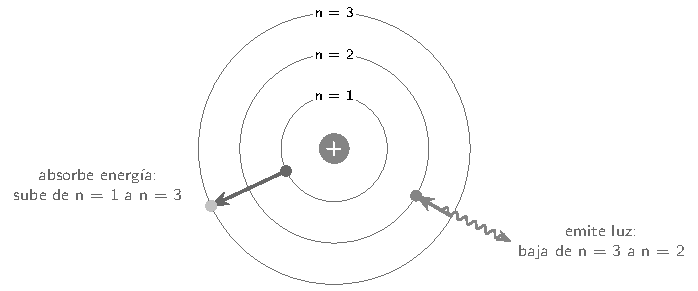
\includegraphics[max width=0.92\linewidth,max height=8.5cm]{qui/atomo_bohr}
\end{center}
\subsection{Lo clave del tema}
\begin{center}\small
\begin{tabularx}{\linewidth}{@{}>{\raggedright\arraybackslash\hsize=0.52\hsize}X>{\raggedright\arraybackslash\hsize=1.04\hsize}X>{\raggedright\arraybackslash\hsize=1.22\hsize}X>{\raggedright\arraybackslash\hsize=1.22\hsize}X@{}}
\toprule
\textbf{Modelo} & \textbf{Evidencia} & \textbf{Qué aporta} & \textbf{Limitación} \\
\midrule
Dalton (1808) & leyes de la masa en las reacciones & átomos indivisibles que se reordenan & el átomo es divisible; hay isótopos \\
Thomson (1904) & rayos catódicos & electrones (\ensuremath{-}) en una esfera positiva & no explica los rebotes de partículas alfa \\
Rutherford (1911) & lámina de oro y partículas alfa & núcleo pequeño, denso y positivo; espacio vacío & el electrón caería al núcleo; no explica los espectros \\
Bohr (1913) & espectros de líneas & niveles de energía fijos; absorción y emisión & solo funciona bien para el hidrógeno \\
\bottomrule
\end{tabularx}
\end{center}
 
\begin{clave}[{Recuerda}] · Thomson descubrió el electrón; Rutherford propuso el núcleo.\par · Casi todas las partículas alfa pasan derecho porque el átomo es casi vacío; unas pocas rebotan al chocar con el núcleo, denso y positivo.\par · Las partículas alfa se desvían por la repulsión del núcleo positivo; los electrones son muy livianos para desviarlas.\par · El electrón absorbe energía al subir de nivel y emite luz al bajar.\par · Los electrones más lejanos son los más fáciles de arrancar.\end{clave}
 
\begin{clave}[{Método PAES}] 1. Identifica de qué modelo habla el texto por su experimento o su idea clave (rayos catódicos \ensuremath{\rightarrow} Thomson; lámina de oro \ensuremath{\rightarrow} Rutherford; niveles y espectros \ensuremath{\rightarrow} Bohr). 2. Une cada observación con la conclusión que permite. 3. Descarta las alternativas que mezclan ideas de modelos distintos o que son ciertas pero no salen de lo descrito.\end{clave}
\begin{elejemplo}{PAES Invierno 2026, adaptada}
A comienzos del siglo XX, un científico propuso un modelo atómico formado por un núcleo y electrones girando a su alrededor. El modelo surgió de un experimento en el que se lanzaron partículas alfa, de carga positiva, contra una lámina muy delgada de oro:

La gran mayoría de las partículas atravesó la lámina sin cambiar su trayectoria. Unas pocas se desviaron y, aproximadamente, una de cada cien mil rebotó en dirección contraria.

De acuerdo con lo anterior, ¿cuál de las siguientes inferencias es correcta?
\begin{center}
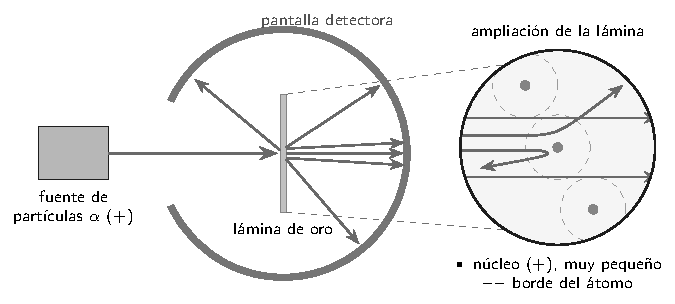
\includegraphics[max width=0.92\linewidth,max height=8.5cm]{qui/atomo_rutherford}
\end{center}
\altslargas{El átomo tiene un núcleo que ocupa casi todo su volumen.}{Los electrones del átomo repelen a las partículas alfa.}{El átomo está formado principalmente por espacio vacío.}{El núcleo del átomo tiene carga negativa.}
\solucion{\textbf{Paso 1. ¿Qué nos piden?} Una inferencia que se apoye en las observaciones del experimento de Rutherford. Unimos cada observación con lo que permite concluir.

\textbf{Paso 2. «La gran mayoría pasa sin desviarse».} Si casi todas las partículas atraviesan los miles de capas de átomos de la lámina sin chocar con nada, dentro del átomo casi no hay nada que se interponga: el átomo es principalmente \textbf{espacio vacío}.

\textbf{Paso 3. «Unas pocas se desvían».} Las partículas alfa son positivas. Si algo las desvía, es una zona con carga \textbf{positiva} que las repele.

\textbf{Paso 4. «Una de cada cien mil rebota».} Para hacer rebotar a una partícula tan rápida, esa zona tiene que ser muy densa. Y como casi nunca se choca con ella, debe ser muy pequeña: es el núcleo.

\textbf{Respuesta:} el átomo está formado principalmente por espacio vacío.

\textbf{Comprobación:} si el núcleo fuera grande, muchas partículas chocarían con él y rebotarían; pero rebota solo 1 de cada 100.000, así que el núcleo ocupa una parte ínfima del volumen.

\textbf{¿Por qué no las otras?} «Un núcleo que ocupa casi todo el volumen» contradice que casi todas las partículas pasen. Los electrones tienen carga negativa: atraerían a las partículas alfa, no las repelerían, y además son tan livianos que no pueden desviarlas. Un núcleo negativo atraería a las partículas alfa; no las haría rebotar.

\textbf{\color{cienciaD}Para recordar.} Pasan derecho \ensuremath{\rightarrow} espacio vacío. Se desvían o rebotan \ensuremath{\rightarrow} núcleo pequeño, denso y positivo.}{C}
\end{elejemplo}

%% =====================================================================
%% qui_particulas
\section[Protones, neutrones y electrones]{Protones, neutrones y electrones}
\modcomun\ \ {\color{gris}\itshape Las partículas del átomo, el número atómico Z y el número másico A, la notación de núclido, los isótopos y los iones (cationes y aniones), y cómo contar protones, neutrones y electrones en símbolos y diagramas.\par}
\subsection{Las tres partículas del átomo}
Todo átomo tiene un \textbf{núcleo} muy pequeño, con protones y neutrones, y alrededor, los \textbf{electrones}.

 
\begin{center}\small
\begin{tabular}{@{}llll@{}}
\toprule
\textbf{Partícula} & \textbf{Carga} & \textbf{Masa relativa} & \textbf{Ubicación} \\
\midrule
Protón (p\textsuperscript{+}) & +1 & 1 u & núcleo \\
Neutrón (n\textsuperscript{0}) & 0 & 1 u & núcleo \\
Electrón (e\textsuperscript{\ensuremath{-}}) & \ensuremath{-}1 & casi 0 (1/1840 u) & niveles, fuera del núcleo \\
\bottomrule
\end{tabular}
\end{center}
 

Dos consecuencias:

 
\begin{itemize}
  \item La \textbf{masa} del átomo está casi toda en el núcleo: protones y neutrones.
  \item La \textbf{carga} depende de protones y electrones. Si hay tantos electrones como protones, las cargas se anulan y el átomo es \textbf{neutro}.
\end{itemize}
  
\begin{center}
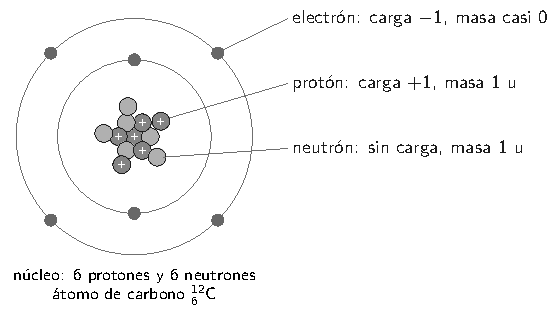
\includegraphics[max width=0.92\linewidth,max height=8.5cm]{qui/atomo_partes}
\end{center}
 
\begin{ojo}[{Ojo}] Los neutrones no tienen carga, pero sí masa: cuentan para la masa del átomo y no cuentan para su carga.\end{ojo}
\subsection{Número atómico Z y número másico A}
\textbf{Número atómico (Z):} la cantidad de \textbf{protones}. Es el «carnet de identidad» del elemento: todos los átomos de carbono tienen 6 protones, y cualquier átomo con 6 protones es carbono. La tabla periódica ordena los elementos según Z.

 

\textbf{Número másico (A):} la cantidad de \textbf{protones más neutrones}, las partículas del núcleo.

 \[ A = Z + n \qquad\Rightarrow\qquad n = A - Z \] 

\textbf{Notación de núclido:} A arriba a la izquierda, Z abajo a la izquierda y la carga, si la hay, arriba a la derecha: $\,{}^{A}_{Z}\text{X}^{\text{carga}}$.

 

En un átomo \textbf{neutro}, electrones = protones = Z.

  
\begin{ejemplo}[{Ejemplo resuelto}] $\,{}^{23}_{11}\text{Na}$.\par \textbf{Paso 1.} Protones: Z = 11.\par \textbf{Paso 2.} Neutrones: $23 - 11 = 12$.\par \textbf{Paso 3.} Electrones: no tiene carga, así que es neutro: 11.\end{ejemplo}
 
\begin{ojo}[{Error típico}] Confundir Z con A, o creer que los neutrones son iguales a los protones. En $\,{}^{35}_{17}\text{Cl}$ hay 17 protones y $35 - 17 = 18$ neutrones.\end{ojo}
 
\begin{clave}[{Masa atómica de la tabla}] No es un número entero (Cl = 35,5) porque es un promedio de los isótopos naturales del elemento. El número másico A, en cambio, siempre es entero.\end{clave}
\subsection{Iones: cationes y aniones}
Un \textbf{ion} es un átomo (o grupo de átomos) con carga eléctrica, porque \textbf{ganó o perdió electrones}. Los protones no cambian: siguen siendo los mismos, y por eso el elemento sigue siendo el mismo.

 
\begin{itemize}
  \item \textbf{Catión} (carga +): \textbf{perdió} electrones. Na\textsuperscript{+}: 11 protones y 10 electrones.
  \item \textbf{Anión} (carga \ensuremath{-}): \textbf{ganó} electrones. Cl\textsuperscript{\ensuremath{-}}: 17 protones y 18 electrones.
\end{itemize}
 

La regla para contar electrones:

 \[ \text{electrones} = Z - \text{carga} \] 

Con carga 2+: $Z - 2$. Con carga 2\ensuremath{-}: $Z - (-2) = Z + 2$.

  
\begin{ejemplo}[{Ejemplo resuelto}] $\,{}^{40}_{20}\text{Ca}^{2+}$.\par \textbf{Paso 1.} Protones: 20.\par \textbf{Paso 2.} Neutrones: $40 - 20 = 20$.\par \textbf{Paso 3.} Electrones: carga 2+, perdió 2: $20 - 2 = 18$.\end{ejemplo}
 
\begin{ejemplo}[{Ejemplo resuelto}] $\,{}^{32}_{16}\text{S}^{2-}$: 16 protones, $32 - 16 = 16$ neutrones y $16 + 2 = 18$ electrones.\end{ejemplo}
 
\begin{ojo}[{Error típico}] «El catión ganó protones». No: un ion nunca cambia sus protones. Si cambiaran los protones, sería otro elemento. Y el signo engaña: carga + significa \textbf{menos} electrones.\end{ojo}
\subsection{Isótopos, isóbaros e isótonos}
\textbf{Isótopos:} átomos del \textbf{mismo elemento} (igual Z) con distinto número de neutrones y, por eso, distinto A. Tienen las mismas propiedades químicas, porque tienen los mismos protones y electrones; solo cambia su masa.

 
\begin{itemize}
  \item Carbono: $\,{}^{12}_{6}\text{C}$ (6 n), $\,{}^{13}_{6}\text{C}$ (7 n) y $\,{}^{14}_{6}\text{C}$ (8 n). El carbono 14 se usa para datar restos arqueológicos.
  \item Hidrógeno: protio $\,{}^{1}_{1}\text{H}$ (0 n), deuterio $\,{}^{2}_{1}\text{H}$ (1 n) y tritio $\,{}^{3}_{1}\text{H}$ (2 n).
\end{itemize}
 

La PAES a veces define otras dos palabras en el enunciado:

 
\begin{itemize}
  \item \textbf{Isóbaros:} igual A, distinto Z (elementos distintos): $\,{}^{40}_{18}\text{Ar}$ y $\,{}^{40}_{20}\text{Ca}$.
  \item \textbf{Isótonos:} igual número de neutrones: $\,{}^{39}_{19}\text{K}$ y $\,{}^{40}_{20}\text{Ca}$ (20 n cada uno).
\end{itemize}
  
\begin{center}\small
\begin{tabular}{@{}llll@{}}
\toprule
\textbf{Comparación} & \textbf{Z (protones)} & \textbf{A} & \textbf{Neutrones} \\
\midrule
Isótopos & igual & distinto & distinto \\
Isóbaros & distinto & igual & distinto \\
Isótonos & distinto & distinto & igual \\
\bottomrule
\end{tabular}
\end{center}
 
\begin{ejemplo}[{Ejemplo resuelto}] ¿En qué se diferencian $\,{}^{28}_{14}\text{Si}$, $\,{}^{29}_{14}\text{Si}$ y $\,{}^{30}_{14}\text{Si}$? Tienen igual Z (14 protones) y, como son neutros, 14 electrones. Se diferencian en los neutrones: 14, 15 y 16. Son isótopos.\end{ejemplo}
\subsection{Contar partículas en un diagrama}
En la PAES aparecen diagramas de Bohr con el núcleo y los electrones dibujados como puntos en sus niveles. Para leerlos:

 

\textbf{Paso 1.} Lee en el núcleo los protones (p) y los neutrones (n).

 

\textbf{Paso 2.} Cuenta los electrones de todos los niveles.

 

\textbf{Paso 3.} Compara: si hay más electrones que protones, es un anión; si hay menos, un catión; si son iguales, un átomo neutro.

 

\textbf{Paso 4.} Arma la notación: Z = protones, A = protones + neutrones, carga = protones \ensuremath{-} electrones.

 

Si el diagrama muestra solo neutrones y dice que el átomo es neutro, los protones son iguales a los electrones que cuentas.

  
\begin{center}
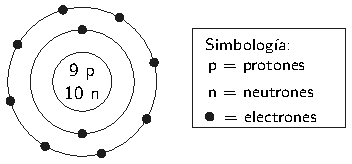
\includegraphics[max width=0.92\linewidth,max height=8.5cm]{qui/atomo_fluoruro}
\end{center}
 
\begin{ejemplo}[{Ejemplo resuelto}] En el diagrama: 9 p y 10 n en el núcleo; electrones: $2 + 8 = 10$. Z = 9, A = 9 + 10 = 19 y carga = 9 \ensuremath{-} 10 = \ensuremath{-}1. Es $\,{}^{19}_{9}\text{X}^{-}$: el ion fluoruro, F\textsuperscript{\ensuremath{-}}.\end{ejemplo}
\subsection{Lo clave del tema}
\begin{center}\small
\begin{tabularx}{\linewidth}{@{}>{\raggedright\arraybackslash\hsize=0.72\hsize}X>{\raggedright\arraybackslash\hsize=0.67\hsize}X>{\raggedright\arraybackslash\hsize=1.61\hsize}X@{}}
\toprule
\textbf{Quiero saber} & \textbf{Cómo lo calculo} & \textbf{Ejemplo: $\,{}^{56}_{26}\text{Fe}^{3+}$} \\
\midrule
Protones & Z & 26 \\
Neutrones & A \ensuremath{-} Z & 56 \ensuremath{-} 26 = 30 \\
Electrones & Z \ensuremath{-} carga & 26 \ensuremath{-} 3 = 23 \\
¿Mismo elemento? & mismo Z & todo átomo con 26 protones es hierro \\
\bottomrule
\end{tabularx}
\end{center}
 
\begin{clave}[{Recuerda}] · Neutrones = A \ensuremath{-} Z.\par · Una carga positiva indica electrones perdidos: Fe\textsuperscript{3+} tiene 26 \ensuremath{-} 3 = 23 electrones.\par · En un ion solo cambian los electrones; los protones definen el elemento.\par · Los isótopos tienen igual Z y distinto número de neutrones.\par · Neutrones y protones pueden ser distintos: $\,{}^{35}_{17}\text{Cl}$ tiene 18 neutrones.\end{clave}
 
\begin{clave}[{Método PAES}] 1. Haz una tablita con p, n y e de cada especie antes de leer las alternativas. 2. Protones = Z; neutrones = A \ensuremath{-} Z; electrones = Z \ensuremath{-} carga. 3. Para comparar especies, resta fila por fila. 4. Para «mismo elemento» o «isótopos», mira solo Z.\end{clave}
\begin{elejemplo}{PAES Invierno 2026, adaptada}
La siguiente tabla presenta el número de protones de cuatro iones:

A partir de la tabla, ¿cuál de las siguientes comparaciones del número de electrones de los iones es correcta?
\begin{center}\small
\begin{tabular}{@{}ll@{}}
\toprule
\textbf{Ion} & \textbf{N.° de protones} \\
\midrule
\textbf{I\textsuperscript{\ensuremath{-}}} & 53 \\
\textbf{S\textsuperscript{2\ensuremath{-}}} & 16 \\
\textbf{Mg\textsuperscript{2+}} & 12 \\
\textbf{Al\textsuperscript{3+}} & 13 \\
\bottomrule
\end{tabular}
\end{center}
\altslargas{El ion S\textsuperscript{2\ensuremath{-}} tiene 4 electrones más que el ion Mg\textsuperscript{2+}.}{El ion Mg\textsuperscript{2+} tiene 1 electrón menos que el ion Al\textsuperscript{3+}.}{El ion I\textsuperscript{\ensuremath{-}} tiene 36 electrones más que el ion S\textsuperscript{2\ensuremath{-}}.}{El ion Al\textsuperscript{3+} tiene 40 electrones menos que el ion I\textsuperscript{\ensuremath{-}}.}
\solucion{\textbf{Paso 1. ¿Qué nos piden?} Comparar electrones, pero la tabla da protones. Primero calculamos los electrones de cada ion con electrones = protones \ensuremath{-} carga.

\textbf{Paso 2. I\textsuperscript{\ensuremath{-}}.} Carga \ensuremath{-}1: ganó 1 electrón. $53 + 1 = 54$ electrones.

\textbf{Paso 3. S\textsuperscript{2\ensuremath{-}}.} Ganó 2: $16 + 2 = 18$ electrones.

\textbf{Paso 4. Mg\textsuperscript{2+}.} Perdió 2: $12 - 2 = 10$ electrones.

\textbf{Paso 5. Al\textsuperscript{3+}.} Perdió 3: $13 - 3 = 10$ electrones.

\textbf{Paso 6. Compara.} I\textsuperscript{\ensuremath{-}} y S\textsuperscript{2\ensuremath{-}}: $54 - 18 = 36$. \ding{52} S\textsuperscript{2\ensuremath{-}} y Mg\textsuperscript{2+}: $18 - 10 = 8$. Mg\textsuperscript{2+} y Al\textsuperscript{3+}: $10 - 10 = 0$, tienen los mismos. Al\textsuperscript{3+} y I\textsuperscript{\ensuremath{-}}: $54 - 10 = 44$.

\textbf{Respuesta:} el ion I\textsuperscript{\ensuremath{-}} tiene 36 electrones más que el ion S\textsuperscript{2\ensuremath{-}}.

\textbf{Comprobación:} I\textsuperscript{\ensuremath{-}} tiene los mismos electrones que el gas noble xenón (54) y S\textsuperscript{2\ensuremath{-}}, los mismos que el argón (18): $54 - 18 = 36$ \ding{52}.

\textbf{¿Por qué no las otras?} Las otras tres comparan \textbf{protones} en vez de electrones, olvidando la carga: $16 - 12 = 4$, $13 - 12 = 1$ y $53 - 13 = 40$. Con los electrones, las diferencias reales son 8, 0 y 44.

\textbf{\color{cienciaD}Para recordar.} Antes de comparar iones, convierte protones en electrones: electrones = Z \ensuremath{-} carga.}{C}
\end{elejemplo}

\chapter{Química orgánica}
%% =====================================================================
%% qui_carbono
\section[El átomo de carbono]{El átomo de carbono}
\modcomun\ \ {\color{gris}\itshape Por qué el carbono forma cuatro enlaces, cómo contar enlaces sigma y pi, cómo reconocer la hibridación sp³, sp² y sp de cada carbono y cómo cambian la energía, la longitud y el ángulo de enlace.\par}
\subsection{Tetravalencia: el carbono siempre forma 4 enlaces}
El carbono tiene $Z = 6$: su configuración es 1s\textsuperscript{2} 2s\textsuperscript{2} 2p\textsuperscript{2}. Tiene \textbf{4 electrones de valencia} y los comparte todos: forma siempre \textbf{4 enlaces covalentes}. A esto se le llama \textbf{tetravalencia}.

 

Los 4 enlaces pueden repartirse de varias formas: cuatro simples, un doble y dos simples, un triple y un simple, o dos dobles. Lo que nunca cambia es la suma: \textbf{4}.

 

Además, el carbono se une fácilmente con otros carbonos (\textbf{concatenación}): forma cadenas largas, ramificadas y anillos. Por eso existen millones de compuestos orgánicos.

 
\begin{center}\small
\begin{tabular}{@{}ll@{}}
\toprule
\textbf{Átomo} & \textbf{N.º de enlaces que forma} \\
\midrule
C & 4 \\
N & 3 \\
O, S & 2 \\
H, F, Cl, Br, I & 1 \\
\bottomrule
\end{tabular}
\end{center}
  
\begin{ejemplo}[{Ejemplo: revisa una estructura}] En CH\textsubscript{2}=CH--CH\textsubscript{3} (propeno):\par · C1: doble (cuenta 2) + 2 H = 4 \ding{52}\par · C2: doble (2) + 1 H + 1 simple = 4 \ding{52}\par · C3: 1 simple + 3 H = 4 \ding{52}\end{ejemplo}
 
\begin{ojo}[{Error típico}] Contar un enlace doble como 1. Un doble "gasta" 2 de los 4 enlaces del carbono y un triple gasta 3. Por eso el CH de un doble enlace tiene un solo H, y el C de un triple interno no tiene ninguno.\end{ojo}
\subsection{Enlaces simple, doble y triple: sigma y pi}
Cada línea de una fórmula es un par de electrones compartidos. Pero no todos los enlaces son iguales:

 
\begin{itemize}
  \item \textbf{Enlace simple} (C--C, C--H): 1 enlace \textbf{sigma} ($\sigma$).
  \item \textbf{Enlace doble} (C=C, C=O): 1 $\sigma$ + 1 \textbf{pi} ($\pi$).
  \item \textbf{Enlace triple} (C\ensuremath{\equiv}C, C\ensuremath{\equiv}N): 1 $\sigma$ + 2 $\pi$.
\end{itemize}
 

El enlace $\sigma$ une los núcleos de frente; el $\pi$ se forma por los lados, con orbitales p que quedaron sin mezclar. Entre dos átomos hay \textbf{como máximo un} $\sigma$.

 
\begin{clave}[{Método para contar}] 1. Dibuja (o imagina) todos los H. 2. Cada enlace, sea simple, doble o triple, aporta \textbf{exactamente 1} $\sigma$. 3. Los $\pi$ son las líneas extra: 1 por cada doble y 2 por cada triple.\end{clave}
 
\gatotip[\gatonegro]{\textbf{Atajo.} En una molécula sin anillos, n.º de $\sigma$ = n.º de átomos \ensuremath{-} 1. Por cada anillo, suma 1. Benceno C\textsubscript{6}H\textsubscript{6}: $12 - 1 + 1 = 12$ enlaces $\sigma$.}
  
\begin{center}
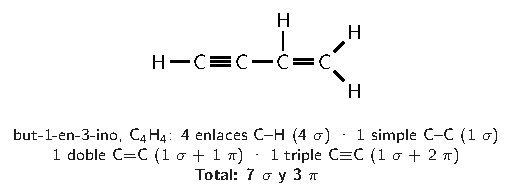
\includegraphics[max width=0.92\linewidth,max height=8.5cm]{qui/org_sigma_pi}
\end{center}
 
\begin{ojo}[{Error típico}] Contar el triple como 3 $\sigma$, o "olvidar" los C--H porque no se dibujan en la fórmula topológica. Los C--H también son enlaces $\sigma$.\end{ojo}
\subsection{Hibridación: sp³, sp² y sp}
Para formar sus enlaces, el carbono "mezcla" su orbital 2s con orbitales 2p y obtiene orbitales nuevos, iguales entre sí: los \textbf{orbitales híbridos}. Cuántos mezcla depende de cuántos enlaces $\pi$ tenga que formar.

 
\begin{center}
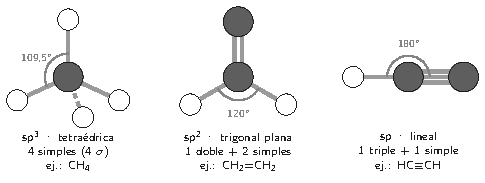
\includegraphics[max width=0.92\linewidth,max height=8.5cm]{qui/org_geometrias}
\end{center}
 
\begin{center}\small
\begin{tabularx}{\linewidth}{@{}>{\raggedright\arraybackslash\hsize=0.76\hsize}X>{\raggedright\arraybackslash\hsize=1.68\hsize}X>{\raggedright\arraybackslash\hsize=0.97\hsize}X>{\raggedright\arraybackslash\hsize=0.76\hsize}X>{\raggedright\arraybackslash\hsize=0.49\hsize}X>{\raggedright\arraybackslash\hsize=1.35\hsize}X@{}}
\toprule
\textbf{Hibridación} & \textbf{Enlaces del C} & \textbf{Átomos unidos al C} & \textbf{Geometría} & \textbf{Ángulo} & \textbf{Ejemplo} \\
\midrule
sp\textsuperscript{3} & 4 simples & 4 & tetraédrica & 109,5° & CH\textsubscript{4}, alcanos, C de un CH\textsubscript{3} \\
sp\textsuperscript{2} & 1 doble + 2 simples & 3 & trigonal plana & 120° & eteno, C=O, benceno \\
sp & 1 triple + 1 simple, o 2 dobles & 2 & lineal & 180° & etino, C\ensuremath{\equiv}N, C del CO\textsubscript{2} \\
\bottomrule
\end{tabularx}
\end{center}
 
\gatotip[\gatoatigrado]{\textbf{Regla rápida.} Mira solo al carbono que te preguntan: \textbf{solo simples \ensuremath{\rightarrow} sp³}; \textbf{un doble \ensuremath{\rightarrow} sp²}; \textbf{un triple o dos dobles \ensuremath{\rightarrow} sp}. También sirve contar los átomos unidos a él: 4 \ensuremath{\rightarrow} sp³, 3 \ensuremath{\rightarrow} sp², 2 \ensuremath{\rightarrow} sp.}
\subsection{Energía, longitud y ángulo de enlace}
Mientras más pares de electrones comparten dos carbonos, más \textbf{cerca} quedan sus núcleos y más \textbf{energía} cuesta separarlos.

 
\begin{center}\small
\begin{tabular}{@{}llll@{}}
\toprule
\textbf{Enlace} & \textbf{Hibridación} & \textbf{Longitud} & \textbf{Energía de enlace} \\
\midrule
C--C & sp\textsuperscript{3} & 154 pm (0,154 nm) & 347 kJ/mol \\
C=C & sp\textsuperscript{2} & 134 pm (0,134 nm) & 614 kJ/mol \\
C\ensuremath{\equiv}C & sp & 120 pm (0,120 nm) & 839 kJ/mol \\
\bottomrule
\end{tabular}
\end{center}
 

\textbf{Longitud de enlace}: distancia entre los núcleos. Disminuye: C--C > C=C > C\ensuremath{\equiv}C.\par \textbf{Energía de enlace}: energía necesaria para romperlo. Aumenta: C--C < C=C < C\ensuremath{\equiv}C.\par \textbf{Ángulo de enlace}: depende de la hibridación (109,5°, 120° o 180°).

  
\begin{ejemplo}[{Ejemplo resuelto}] ¿El doble enlace vale el doble que el simple? $2 \cdot 347 = 694$ kJ/mol, pero el C=C tiene 614. El enlace $\pi$ aporta solo $614 - 347 = 267$ kJ/mol: es \textbf{más débil} que el $\sigma$. Por eso alquenos y alquinos son más reactivos que los alcanos: el $\pi$ se rompe primero.\end{ejemplo}
 
\begin{ojo}[{Ojo con las unidades}] El DEMRE puede dar las longitudes en nm (0,154) o en pm (154). $1\ \text{nm} = 1000\ \text{pm}$. Para comparar, usa la misma unidad en todas.\end{ojo}
 
\begin{ojo}[{Error típico}] Creer que "más enlaces = más largo". Es al revés: el triple es el \textbf{más corto} y el \textbf{más fuerte}.\end{ojo}
\subsection{Ejemplo: hibridación y enlaces átomo por átomo}
El acrilonitrilo, CH\textsubscript{2}=CH--C\ensuremath{\equiv}N, se usa para fabricar fibras acrílicas. Analicemos cada carbono, numerando de izquierda a derecha.

 

\textbf{Paso 1. C1 (CH\textsubscript{2}=).} Tiene un doble enlace y dos H: 3 átomos unidos \ensuremath{\rightarrow} \textbf{sp²}, 120°.

 

\textbf{Paso 2. C2 (=CH--).} Un doble, un H y un simple: 3 átomos unidos \ensuremath{\rightarrow} \textbf{sp²}, 120°.

 

\textbf{Paso 3. C3 (--C\ensuremath{\equiv}N).} Un simple y un triple: 2 átomos unidos \ensuremath{\rightarrow} \textbf{sp}, 180°. Por eso C2, C3 y N están en línea recta.

 

\textbf{Paso 4. Enlaces.} Átomos: 3 C + 3 H + 1 N = 7, sin anillos \ensuremath{\rightarrow} $7 - 1 = 6$ enlaces $\sigma$. Enlaces $\pi$: 1 (del doble) + 2 (del triple) = 3.

 

\textbf{Comprobación:} contando uno por uno: 3 C--H + C1=C2 + C2--C3 + C3\ensuremath{\equiv}N = 6 enlaces, cada uno con 1 $\sigma$. \ding{52}

  
\begin{clave}[{Lo mismo con un grupo carbonilo}] En el ácido acético, CH\textsubscript{3}--COOH: el C del CH\textsubscript{3} es sp³ y el C del COOH es \textbf{sp²}, porque tiene un doble enlace C=O. Los dobles con O o N también cuentan.\end{clave}
 
\begin{ojo}[{Error típico}] Pensar que un C unido a un OH es sp³ "porque el OH es simple". Mira \textbf{todos} sus enlaces: el C del COOH tiene un C=O, así que es sp².\end{ojo}
\subsection{Lo clave del tema}
\begin{center}\small
\begin{tabularx}{\linewidth}{@{}>{\raggedright\arraybackslash\hsize=1.30\hsize}X>{\raggedright\arraybackslash\hsize=0.57\hsize}X>{\raggedright\arraybackslash\hsize=0.81\hsize}X>{\raggedright\arraybackslash\hsize=1.02\hsize}X>{\raggedright\arraybackslash\hsize=1.30\hsize}X@{}}
\toprule
\textbf{Enlaces del carbono} & \textbf{Hibridación} & \textbf{Geometría y ángulo} & \textbf{$\sigma$ y $\pi$ de ese enlace} & \textbf{Longitud / energía} \\
\midrule
4 simples & sp\textsuperscript{3} & tetraédrica, 109,5° & simple: 1 $\sigma$ & C--C: la más larga, la más débil \\
1 doble + 2 simples & sp\textsuperscript{2} & trigonal plana, 120° & doble: 1 $\sigma$ + 1 $\pi$ & C=C: intermedia \\
1 triple + 1 simple (o 2 dobles) & sp & lineal, 180° & triple: 1 $\sigma$ + 2 $\pi$ & C\ensuremath{\equiv}C: la más corta, la más fuerte \\
\bottomrule
\end{tabularx}
\end{center}
  
\begin{clave}[{Recuerda}] · El triple enlace tiene 1 $\sigma$ y 2 $\pi$.\par · Cada C--H es un enlace $\sigma$.\par · El C de un C=O es sp².\par · Más enlaces entre dos átomos: enlace más corto y más fuerte.\end{clave}
  
\begin{clave}[{Método PAES}] 1. Completa los H que faltan (4 enlaces por C). 2. Para hibridación, mira cada carbono por separado y cuenta sus átomos vecinos. 3. Para $\sigma$: un $\sigma$ por cada enlace (o átomos \ensuremath{-} 1, más 1 por anillo). Para $\pi$: 1 por doble, 2 por triple. 4. Revisa si te piden el total o solo los C--C.\end{clave}
\begin{elejemplo}{PAES Invierno 2027, adaptada}
La siguiente figura representa la molécula de etinilbenceno (fenilacetileno), usada en la síntesis de polímeros conductores.

Al respecto, ¿qué opción contiene el número correcto de enlaces de la molécula?
\begin{center}
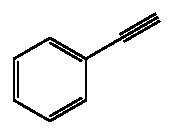
\includegraphics[max width=0.92\linewidth,max height=8.5cm]{qui/org_fenilacetileno}
\end{center}
{\centering\small\color{gris}Etinilbenceno (fórmula topológica)\par}
\alts{8 $\sigma$ (C--C), 5 $\pi$ (C--C) y 6 $\sigma$ (C--H)}{8 $\sigma$ (C--C), 2 $\pi$ (C--C) y 6 $\sigma$ (C--H)}{7 $\sigma$ (C--C), 5 $\pi$ (C--C) y 5 $\sigma$ (C--H)}{10 $\sigma$ (C--C), 5 $\pi$ (C--C) y 6 $\sigma$ (C--H)}
\solucion{\textbf{Paso 1. ¿Qué nos piden?} Tres conteos: enlaces $\sigma$ entre carbonos, enlaces $\pi$ entre carbonos y enlaces $\sigma$ C--H.

 

\textbf{Paso 2. Cuenta los carbonos.} El anillo tiene 6 vértices (6 C) y la cadena lateral tiene 2 C (el vértice unido al anillo y el extremo del triple). Total: 8 C, fórmula C\textsubscript{8}H\textsubscript{6}.

 

\textbf{Paso 3. Enlaces C--C y sus $\sigma$.} En el anillo hay 6 enlaces C--C; el anillo se une a la cadena con 1 enlace; y el triple es 1 enlace más. Son 8 enlaces C--C, y cada uno tiene exactamente 1 $\sigma$: \textbf{8 $\sigma$ (C--C)}.

 

\textbf{Paso 4. Enlaces $\pi$.} El anillo dibujado tiene 3 dobles (3 $\pi$) y el triple aporta 2 $\pi$: \textbf{5 $\pi$}.

 

\textbf{Paso 5. Enlaces C--H.} Completa a 4 enlaces cada C del anillo: el C unido a la cadena tiene 3 vecinos (2 del anillo y 1 de la cadena) y uno de esos enlaces es doble, así que ya suma 4 y no lleva H; los otros 5 C del anillo llevan 1 H cada uno. El C terminal del triple lleva 1 H (3 del triple + 1 H = 4). Total: \textbf{6 $\sigma$ (C--H)}.

 

\textbf{Respuesta:} 8 $\sigma$ (C--C), 5 $\pi$ (C--C) y 6 $\sigma$ (C--H).

 

\textbf{Comprobación:} la molécula tiene $8 + 6 = 14$ átomos y 1 anillo, así que debe tener $14 - 1 + 1 = 14$ enlaces $\sigma$ en total: $8 + 6 = 14$. \ding{52}

 

\textbf{¿Por qué no las otras?} "2 $\pi$" cuenta solo el triple y olvida los 3 dobles del anillo. "7 $\sigma$ y 5 C--H" olvida el enlace entre el anillo y la cadena, y el H del extremo del triple. "10 $\sigma$" cuenta el triple como 3 enlaces $\sigma$, pero un triple tiene 1 $\sigma$ y 2 $\pi$.

\textbf{\color{cienciaD}Para recordar.} Cada enlace (simple, doble o triple) aporta un solo sigma; los pi son las líneas extra: 1 por doble y 2 por triple.}{A}
\end{elejemplo}

%% =====================================================================
%% qui_representaciones
\section[Modelos de representación de moléculas]{Modelos de representación de moléculas}
\modcomun\ \ {\color{gris}\itshape Fórmula molecular, empírica, desarrollada, semidesarrollada, condensada y topológica, y los modelos de esferas y varillas y compacto: qué muestra cada una y cómo pasar de una a otra contando C e H.\par}
\subsection{Fórmula molecular y fórmula empírica}
La \textbf{fórmula molecular} dice qué átomos tiene una molécula y \textbf{cuántos exactamente}. El butano es C\textsubscript{4}H\textsubscript{10}: 4 C y 10 H.

 

La \textbf{fórmula empírica} da solo la \textbf{proporción mínima entera} entre los átomos. Se obtiene dividiendo todos los subíndices por su máximo común divisor (MCD).

 

\textbf{Paso 1.} Escribe la fórmula molecular: C\textsubscript{6}H\textsubscript{12}O\textsubscript{6} (glucosa).\par \textbf{Paso 2.} Busca el MCD de 6, 12 y 6: es 6.\par \textbf{Paso 3.} Divide: C\textsubscript{1}H\textsubscript{2}O\textsubscript{1} \ensuremath{\rightarrow} \textbf{CH\textsubscript{2}O}.

 
\begin{center}\small
\begin{tabular}{@{}lll@{}}
\toprule
\textbf{Compuesto} & \textbf{Molecular} & \textbf{Empírica} \\
\midrule
butano & C\textsubscript{4}H\textsubscript{10} & C\textsubscript{2}H\textsubscript{5} \\
benceno & C\textsubscript{6}H\textsubscript{6} & CH \\
etino & C\textsubscript{2}H\textsubscript{2} & CH \\
ácido etanoico & C\textsubscript{2}H\textsubscript{4}O\textsubscript{2} & CH\textsubscript{2}O \\
cloroformo & CHCl\textsubscript{3} & CHCl\textsubscript{3} \\
\bottomrule
\end{tabular}
\end{center}
  
\begin{clave}[{Ya es mínima}] Si el MCD es 1, la empírica es igual a la molecular. Le pasa al cloroformo (CHCl\textsubscript{3}), a la vanilina (C\textsubscript{8}H\textsubscript{8}O\textsubscript{3}) y al propano (C\textsubscript{3}H\textsubscript{8}).\end{clave}
 
\begin{ojo}[{Error típico}] Dividir solo algunos subíndices, o dividir aunque no den enteros. En C\textsubscript{8}H\textsubscript{8}O\textsubscript{3}, el 3 no se puede dividir por 8: la fórmula ya es empírica.\end{ojo}
 
\begin{ojo}[{Ojo}] Distintas sustancias pueden tener la misma empírica: el etino y el benceno son ambos CH. La empírica sola no identifica un compuesto.\end{ojo}
\subsection{Desarrollada, semidesarrollada, condensada y topológica}
Las fórmulas estructurales muestran, además, \textbf{cómo están unidos} los átomos. Mira las cuatro formas de escribir el butano:

 
\begin{center}
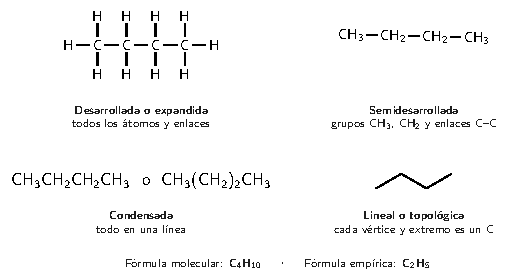
\includegraphics[max width=0.92\linewidth,max height=8.5cm]{qui/org_repr_butano}
\end{center}
  
\begin{itemize}
  \item \textbf{Desarrollada o expandida}: todos los átomos y todos los enlaces, uno por uno.
  \item \textbf{Semidesarrollada}: se agrupan los H con su carbono (CH\textsubscript{3}, CH\textsubscript{2}) y se dibujan los enlaces entre carbonos.
\end{itemize}
  
\begin{itemize}
  \item \textbf{Condensada}: todo en una línea, sin guiones; los grupos repetidos van entre paréntesis.
  \item \textbf{Lineal o topológica}: solo un zig-zag; cada vértice y cada extremo es un carbono.
\end{itemize}
\subsection{Cómo leer una fórmula topológica}
La fórmula topológica es la más usada en la PAES, porque es rápida de dibujar. Sus reglas:

 
\begin{itemize}
  \item Cada \textbf{vértice} y cada \textbf{extremo} de línea es un átomo de C.
  \item Los H unidos a carbono \textbf{no se dibujan}: cada C tiene los H que le faltan para llegar a 4 enlaces.
  \item Los otros átomos (O, N, Cl, S) \textbf{sí se escriben}, con sus H (OH, NH\textsubscript{2}).
  \item Una línea doble es un enlace doble; una triple, un triple.
\end{itemize}
 
\begin{center}
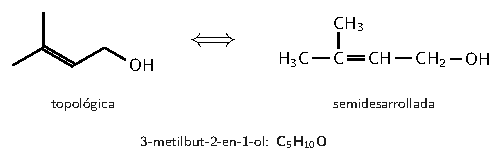
\includegraphics[max width=0.92\linewidth,max height=8.5cm]{qui/org_topo_prenol}
\end{center}
  
\begin{ejemplo}[{Ejemplo resuelto: contar C e H}] En la figura (3-metilbut-2-en-1-ol):\par \textbf{Paso 1. Carbonos.} 2 extremos arriba e izquierda + el vértice que los une + el vértice del doble + el vértice antes del OH = 5 C.\par \textbf{Paso 2. H de cada C} = 4 \ensuremath{-} (enlaces que ya tiene):\par · los dos CH\textsubscript{3} de los extremos: 3 + 3\par · el C con el doble y dos ramas: 4 \ensuremath{-} 4 = 0\par · el =CH--: 4 \ensuremath{-} 3 = 1\par · el CH\textsubscript{2} unido al OH: 4 \ensuremath{-} 2 = 2\par · el H del OH: 1\par \textbf{Paso 3.} Total: $3 + 3 + 0 + 1 + 2 + 1 = 10$ H. Fórmula: \textbf{C\textsubscript{5}H\textsubscript{10}O}.\end{ejemplo}
 
\begin{ojo}[{Errores típicos}] Olvidar los carbonos de los extremos, olvidar el H del OH, o poner H en un carbono que ya tiene 4 enlaces (por ejemplo, el que tiene un doble y dos ramas).\end{ojo}
\subsection{Modelos tridimensionales: esferas y varillas, y compacto}
\begin{center}
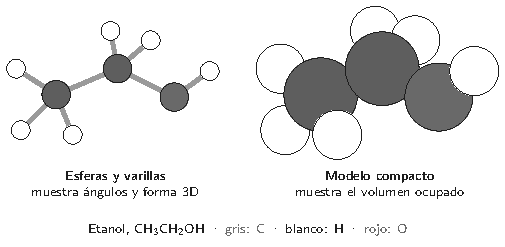
\includegraphics[max width=0.92\linewidth,max height=8.5cm]{qui/org_modelos}
\end{center}
  

\textbf{Modelo de esferas y varillas}: cada átomo es una esfera y cada enlace es una varilla. Muestra la \textbf{forma 3D}, los \textbf{ángulos de enlace} (109,5°, 120°, 180°) y cómo se ordenan los átomos en el espacio.

 

\textbf{Modelo compacto} (o de espacio lleno): las esferas se tocan y se superponen, a escala de su tamaño real. Muestra el \textbf{volumen} y la \textbf{forma externa} de la molécula, pero los enlaces y ángulos se ven poco.

  
\begin{clave}[{Colores habituales}] C: gris o negro · H: blanco · O: rojo · N: azul · Cl: verde.\end{clave}
 
\begin{ojo}[{Clave PAES}] Si dos formas de una molécula se diferencian solo en cómo se ordenan sus átomos \textbf{en el espacio}, ninguna fórmula escrita en el plano (molecular, empírica, condensada) las distingue: se necesita un modelo 3D, como el de esferas y varillas.\end{ojo}
\subsection{Comparar representaciones y moléculas}
\begin{center}\small
\begin{tabularx}{\linewidth}{@{}>{\raggedright\arraybackslash\hsize=1.29\hsize}X>{\raggedright\arraybackslash\hsize=1.29\hsize}X>{\raggedright\arraybackslash\hsize=0.67\hsize}X>{\raggedright\arraybackslash\hsize=0.76\hsize}X@{}}
\toprule
\textbf{Representación} & \textbf{¿Cuántos átomos de cada tipo?} & \textbf{¿Cómo se unen?} & \textbf{¿Forma 3D?} \\
\midrule
Empírica & solo la proporción & no & no \\
Molecular & sí & no & no \\
Condensada / semidesarrollada & sí & sí (por grupos) & no \\
Desarrollada / topológica & sí & sí & no (dibujo plano) \\
Esferas y varillas / compacto & sí & sí & sí \\
\bottomrule
\end{tabularx}
\end{center}
  
\begin{ejemplo}[{Ejemplo resuelto}] Etanol, CH\textsubscript{3}--CH\textsubscript{2}--OH, y metoximetano, CH\textsubscript{3}--O--CH\textsubscript{3}. \textbf{Paso 1.} Cuenta: los dos tienen 2 C, 6 H y 1 O: fórmula molecular C\textsubscript{2}H\textsubscript{6}O. \textbf{Paso 2.} Masa molar (H = 1, C = 12, O = 16): $2 \cdot 12 + 6 \cdot 1 + 16 = 46$ g/mol los dos. \textbf{Paso 3.} Pero la semidesarrollada muestra que son \textbf{distintos}: uno tiene O--H y el otro C--O--C. Son \textbf{isómeros}.\end{ejemplo}
  
\begin{ojo}[{Ojo con la masa molar}] Igual fórmula molecular implica igual masa molar. Pero igual masa molar \textbf{no} implica igual fórmula: el butan-2-ol (C\textsubscript{4}H\textsubscript{10}O) y el ácido propanoico (C\textsubscript{3}H\textsubscript{6}O\textsubscript{2}) pesan ambos 74 g/mol.\end{ojo}
\subsection{Lo clave del tema}
\begin{center}\small
\begin{tabularx}{\linewidth}{@{}>{\raggedright\arraybackslash\hsize=0.90\hsize}X>{\raggedright\arraybackslash\hsize=0.96\hsize}X>{\raggedright\arraybackslash\hsize=1.14\hsize}X@{}}
\toprule
\textbf{Representación} & \textbf{Butano} & \textbf{Lo que la distingue} \\
\midrule
Molecular & C\textsubscript{4}H\textsubscript{10} & número exacto de átomos \\
Empírica & C\textsubscript{2}H\textsubscript{5} & proporción mínima (divide por el MCD) \\
Desarrollada & todos los H y enlaces dibujados & todos los enlaces \\
Semidesarrollada & CH\textsubscript{3}--CH\textsubscript{2}--CH\textsubscript{2}--CH\textsubscript{3} & grupos CH\textsubscript{n} + enlaces C--C \\
Condensada & CH\textsubscript{3}(CH\textsubscript{2})\textsubscript{2}CH\textsubscript{3} & una línea, sin enlaces \\
Topológica & zig-zag de 4 vértices & vértices y extremos = C; H implícitos \\
Esferas y varillas / compacto & modelo 3D & ángulos / volumen \\
\bottomrule
\end{tabularx}
\end{center}
  
\begin{clave}[{Recuerda}] · En la fórmula topológica, cada extremo es un CH\textsubscript{3} (si no hay otro átomo escrito).\par · C\textsubscript{8}H\textsubscript{8}O\textsubscript{3} ya es empírica: el MCD de 8, 8 y 3 es 1.\par · Isómeros = misma fórmula molecular.\end{clave}
  
\begin{clave}[{Método PAES para contar}] 1. Marca cada vértice y extremo (C). 2. Para cada C: H = 4 \ensuremath{-} enlaces dibujados (doble cuenta 2, triple cuenta 3). 3. Suma los H de OH, NH\textsubscript{2}, CHO escritos. 4. Escribe C, H y luego los demás átomos. 5. Si piden la empírica, divide por el MCD.\end{clave}
\begin{elejemplo}{PAES Invierno 2026, adaptada}
Durante una clase de química orgánica, cuatro estudiantes analizan las estructuras de los compuestos X, Y y Z (masas atómicas: H = 1, C = 12, O = 16):

Luego, cada uno escribe en su cuaderno lo siguiente:

Estudiante 1: X e Y tienen la misma fórmula molecular.\par Estudiante 2: Z tiene más átomos de carbono que X.\par Estudiante 3: X y Z tienen la misma fórmula molecular, porque tienen la misma masa molar.\par Estudiante 4: Y tiene el doble de átomos de hidrógeno que Z.

¿Cuál de los estudiantes escribe una conclusión correcta?
\begin{center}
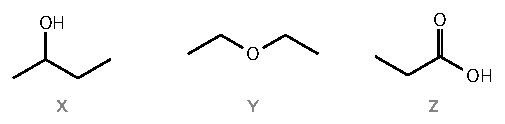
\includegraphics[max width=0.92\linewidth,max height=8.5cm]{qui/org_xyz}
\end{center}
\alts{El estudiante 1.}{El estudiante 2.}{El estudiante 3.}{El estudiante 4.}
\solucion{\textbf{Paso 1. ¿Qué nos piden?} La única afirmación correcta. Para eso necesitamos la fórmula molecular de X, Y y Z.

 

\textbf{Paso 2. Compuesto X.} Cuatro vértices/extremos: 4 C. H: extremo izquierdo CH\textsubscript{3} (3), vértice con OH: tiene 2 C y el O, le falta 1 H (1), siguiente vértice CH\textsubscript{2} (2), extremo CH\textsubscript{3} (3), más el H del OH (1). Total 10 H. \textbf{X = C\textsubscript{4}H\textsubscript{10}O} (butan-2-ol).

 

\textbf{Paso 3. Compuesto Y.} Dos C a cada lado del O: 4 C. Extremos CH\textsubscript{3} (3 + 3) y vértices junto al O, CH\textsubscript{2} (2 + 2). Total 10 H. \textbf{Y = C\textsubscript{4}H\textsubscript{10}O} (etoxietano).

 

\textbf{Paso 4. Compuesto Z.} 3 C: extremo CH\textsubscript{3} (3), vértice CH\textsubscript{2} (2) y el C del COOH (0 H sobre el C), más el H del OH (1). Total 6 H. \textbf{Z = C\textsubscript{3}H\textsubscript{6}O\textsubscript{2}} (ácido propanoico).

 

\textbf{Paso 5. Revisa cada estudiante.} 1: X e Y son ambos C\textsubscript{4}H\textsubscript{10}O. \ding{52} 2: Z tiene 3 C y X tiene 4. \ding{56} 3: X (C\textsubscript{4}H\textsubscript{10}O) y Z (C\textsubscript{3}H\textsubscript{6}O\textsubscript{2}) son fórmulas distintas. \ding{56} 4: Y tiene 10 H y Z tiene 6; el doble de 6 sería 12. \ding{56}

 

\textbf{Respuesta:} el estudiante 1.

 

\textbf{Comprobación:} masas molares: X = $4 \cdot 12 + 10 + 16 = 74$ g/mol; Z = $3 \cdot 12 + 6 + 2 \cdot 16 = 74$ g/mol. Tienen igual masa molar, pero distinta fórmula: por eso el estudiante 3 se equivoca, aunque su dato de masa sea cierto.

 

\textbf{¿Por qué no las otras?} El estudiante 2 no cuenta el carbono del extremo izquierdo de X o cuenta uno de más en Z. El estudiante 3 confunde "misma masa molar" con "misma fórmula". El estudiante 4 olvida que el doble de 6 es 12, no 10.

\textbf{\color{cienciaD}Para recordar.} Para comparar moléculas dibujadas, primero escribe la fórmula molecular de cada una: igual masa molar no significa igual fórmula.}{A}
\end{elejemplo}

%% =====================================================================
%% qui_hidrocarburos
\section[Hidrocarburos y nomenclatura IUPAC]{Hidrocarburos y nomenclatura IUPAC}
\modcomun\ \ {\color{gris}\itshape Alcanos, alquenos, alquinos, cíclicos y aromáticos: sus fórmulas generales, cómo encontrar la cadena principal, cómo numerarla y nombrar con ramificaciones, y qué son los isómeros.\par}
\subsection{Clasificación de los hidrocarburos}
Los \textbf{hidrocarburos} son compuestos formados \textbf{solo por C e H}. Son la base del petróleo, del gas natural y de los combustibles.

 
\begin{itemize}
  \item \textbf{Alifáticos} (cadena abierta, lineal o ramificada): 
\begin{itemize}
  \item \textbf{alcanos}: solo enlaces simples (\textbf{saturados}), sufijo \textbf{-ano};
  \item \textbf{alquenos}: al menos un C=C, sufijo \textbf{-eno};
  \item \textbf{alquinos}: al menos un C\ensuremath{\equiv}C, sufijo \textbf{-ino}.
\end{itemize}
  \item \textbf{Cíclicos}: la cadena se cierra en un anillo (prefijo \textbf{ciclo-}): ciclopropano, ciclohexano, ciclohexeno.
  \item \textbf{Aromáticos}: tienen el anillo del \textbf{benceno}.
\end{itemize}
 

Alquenos y alquinos son \textbf{insaturados}: tienen enlaces $\pi$ y dan reacciones de adición (por ejemplo, con H\textsubscript{2} o Br\textsubscript{2}).

  
\begin{center}
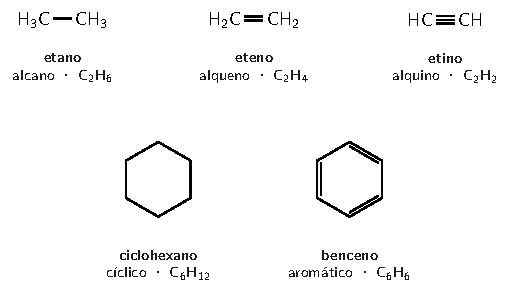
\includegraphics[max width=0.92\linewidth,max height=8.5cm]{qui/org_familias}
\end{center}
\subsection{Fórmulas generales y prefijos}
\begin{center}\small
\begin{tabular}{@{}lll@{}}
\toprule
\textbf{Familia} & \textbf{Fórmula general} & \textbf{Ejemplo} \\
\midrule
Alcano & C\textsubscript{n}H\textsubscript{2n+2} & propano C\textsubscript{3}H\textsubscript{8} \\
Alqueno (un doble) & C\textsubscript{n}H\textsubscript{2n} & propeno C\textsubscript{3}H\textsubscript{6} \\
Alquino (un triple) & C\textsubscript{n}H\textsubscript{2n\ensuremath{-}2} & propino C\textsubscript{3}H\textsubscript{4} \\
Cicloalcano & C\textsubscript{n}H\textsubscript{2n} & ciclopropano C\textsubscript{3}H\textsubscript{6} \\
Benceno & C\textsubscript{6}H\textsubscript{6} & --- \\
\bottomrule
\end{tabular}
\end{center}
 
\begin{clave}[{Regla de los 2 H}] Parte del alcano (C\textsubscript{n}H\textsubscript{2n+2}) y resta \textbf{2 H} por cada doble enlace o anillo, y \textbf{4 H} por cada triple. Ejemplo: C\textsubscript{6}H\textsubscript{10} = $14 - 4$: puede ser un hexino, un hexadieno o un ciclohexeno.\end{clave}
  
\begin{center}\small
\begin{tabular}{@{}llll@{}}
\toprule
\textbf{N.º de C} & \textbf{Prefijo} & \textbf{N.º de C} & \textbf{Prefijo} \\
\midrule
1 & met- & 6 & hex- \\
2 & et- & 7 & hept- \\
3 & prop- & 8 & oct- \\
4 & but- & 9 & non- \\
5 & pent- & 10 & dec- \\
\bottomrule
\end{tabular}
\end{center}
 
\begin{ojo}[{Ojo}] Un alqueno y un cicloalcano con los mismos C tienen la misma fórmula: el propeno y el ciclopropano son ambos C\textsubscript{3}H\textsubscript{6}.\end{ojo}
\subsection{Nombrar cadenas sin ramificar: la convención que usamos}
En este curso usamos las \textbf{recomendaciones IUPAC vigentes}, las mismas de las pruebas DEMRE: el número que indica la posición del doble o triple enlace (el \textbf{localizador}) va \textbf{justo antes del sufijo}.

 

\textbf{Paso 1.} Cuenta los C de la cadena que contiene el enlace múltiple: da el prefijo.\par \textbf{Paso 2.} Numera desde el extremo más cercano al enlace múltiple.\par \textbf{Paso 3.} Escribe prefijo + localizador + sufijo.

 
\begin{center}\small
\begin{tabular}{@{}ll@{}}
\toprule
\textbf{Estructura} & \textbf{Nombre} \\
\midrule
CH\textsubscript{2}=CH--CH\textsubscript{2}--CH\textsubscript{3} & but-1-eno \\
CH\textsubscript{3}--CH=CH--CH\textsubscript{3} & but-2-eno \\
CH\textsubscript{3}--C\ensuremath{\equiv}C--CH\textsubscript{2}--CH\textsubscript{3} & pent-2-ino \\
CH\textsubscript{2}=CH--CH=CH\textsubscript{2} & buta-1,3-dieno \\
\bottomrule
\end{tabular}
\end{center}
  
\begin{ojo}[{Nombres antiguos}] En libros más antiguos verás "2-buteno", "1-butino" o "2-pentino": son los \textbf{mismos compuestos} que but-2-eno, but-1-ino y pent-2-ino. Solo cambia dónde se escribe el número. En la PAES aparece la forma nueva ("penta-2-ino", "butan-2-ona").\end{ojo}
 
\begin{clave}[{Detalles de escritura}] Con dos dobles se agrega una "a" al prefijo: \textbf{buta}-1,3-dieno. Si hay doble y triple, el "-eno" va antes: pent-1-en-3-ino. Con 1 o 2 carbonos no hace falta localizador: eteno, etino, propeno.\end{clave}
 
\begin{clave}[{Grupos alquilo (ramificaciones)}] --CH\textsubscript{3} metil · --CH\textsubscript{2}CH\textsubscript{3} etil · --CH\textsubscript{2}CH\textsubscript{2}CH\textsubscript{3} propil · --CH(CH\textsubscript{3})\textsubscript{2} isopropil.\end{clave}
\subsection{Nombrar con ramificaciones, paso a paso}
\begin{center}
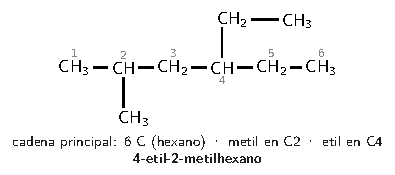
\includegraphics[max width=0.92\linewidth,max height=8.5cm]{qui/org_nom_ejemplo}
\end{center}
  

\textbf{Paso 1. Cadena principal.} La más larga (y, si hay dobles o triples, la que los contiene). Aquí: 6 C \ensuremath{\rightarrow} \textbf{hexano}. Ojo: la cadena más larga puede doblar por una ramificación; no tiene que ser la horizontal.

 

\textbf{Paso 2. Numera} desde el extremo que dé los números más bajos: primero al enlace múltiple; si no hay, a las ramificaciones. Desde la izquierda: 2 y 4. Desde la derecha: 3 y 5. Gana la izquierda.

 

\textbf{Paso 3. Nombra las ramificaciones}: metil en C2, etil en C4.

 

\textbf{Paso 4. Ordena alfabéticamente} (etil antes que metil) y escribe: \textbf{4-etil-2-metilhexano}.

  
\begin{clave}[{Más reglas}] · Ramificaciones repetidas: di-, tri-, tetra-: 2,3-dimetilbutano. Estos prefijos no cuentan para el orden alfabético.\par · Números con comas entre sí y guion entre número y letra: 2,2-dimetilpropano.\par · Si dos cadenas igual de largas compiten, se elige la que tiene más ramificaciones.\end{clave}
 
\begin{ejemplo}[{Ejemplo con doble enlace}] CH\textsubscript{2}=C(CH\textsubscript{3})--CH\textsubscript{2}--CH\textsubscript{3}: cadena de 4 C con el doble; se numera desde el doble (C1). Metil en C2: \textbf{2-metilbut-1-eno}.\end{ejemplo}
\subsection{Hidrocarburos cíclicos y aromáticos}
\textbf{Cicloalcanos}: anillos de C con solo enlaces simples. Se nombran con \textbf{ciclo-} + el nombre del alcano: ciclopropano, ciclopentano, ciclohexano (C\textsubscript{6}H\textsubscript{12}). Con una ramificación: metilciclohexano.

 

\textbf{Aromáticos}: contienen el \textbf{benceno}, C\textsubscript{6}H\textsubscript{6}. Se dibuja con tres dobles alternados o con un círculo dentro del hexágono: sus electrones $\pi$ están \textbf{deslocalizados} en todo el anillo. Por eso el benceno es muy estable y, a diferencia de los alquenos, da reacciones de \textbf{sustitución} y no de adición.

 

Los 6 C del benceno son sp², el anillo es plano y sus ángulos miden 120°.

  
\begin{center}\small
\begin{tabularx}{\linewidth}{@{}>{\raggedright\arraybackslash\hsize=0.97\hsize}X>{\raggedright\arraybackslash\hsize=0.42\hsize}X>{\raggedright\arraybackslash\hsize=1.61\hsize}X@{}}
\toprule
\textbf{Aromático} & \textbf{Fórmula} & \textbf{Uso} \\
\midrule
benceno & C\textsubscript{6}H\textsubscript{6} & materia prima industrial (tóxico) \\
tolueno (metilbenceno) & C\textsubscript{7}H\textsubscript{8} & solvente de pinturas \\
estireno (vinilbenceno) & C\textsubscript{8}H\textsubscript{8} & fabricación de plumavit (poliestireno) \\
naftaleno & C\textsubscript{10}H\textsubscript{8} & antiguas bolitas de naftalina \\
\bottomrule
\end{tabularx}
\end{center}
 
\begin{ojo}[{Error típico}] Contar 2 H en cada C del benceno, como si fuera ciclohexano. En el benceno cada C tiene 1 H (o 0 si lleva un sustituyente).\end{ojo}
\subsection{Isómeros y temperatura de ebullición}
Los \textbf{isómeros} tienen la \textbf{misma fórmula molecular} pero \textbf{distinta estructura}, y por eso distintas propiedades.

 
\begin{itemize}
  \item \textbf{De cadena}: cambia el esqueleto. Butano y metilpropano (C\textsubscript{4}H\textsubscript{10}).
  \item \textbf{De posición}: cambia la ubicación del doble enlace o del grupo. But-1-eno y but-2-eno.
  \item \textbf{De función}: cambia el tipo de compuesto. Etanol y metoximetano (C\textsubscript{2}H\textsubscript{6}O); hex-1-eno y ciclohexano (C\textsubscript{6}H\textsubscript{12}).
\end{itemize}
 
\begin{clave}[{Dos tendencias que pregunta la PAES}] 1. En una serie de alcanos lineales, \textbf{a más carbonos, mayor temperatura de ebullición} (más superficie de contacto entre moléculas).\par 2. Entre isómeros, \textbf{a más ramificación, menor temperatura de ebullición} (la molécula es más compacta y se atrae menos con sus vecinas).\end{clave}
  
\begin{center}
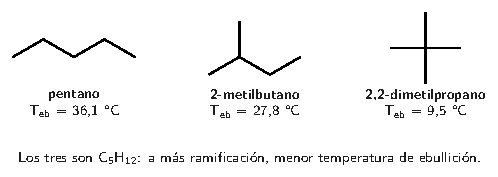
\includegraphics[max width=0.92\linewidth,max height=8.5cm]{qui/org_isomeros_c5}
\end{center}
 
\begin{ojo}[{Ojo}] "3-metilbutano" no existe como nombre: numerado bien, es el 2-metilbutano. Y "1-metilbutano" es en realidad el pentano. Antes de contar isómeros, nombra cada uno para no repetir.\end{ojo}
\subsection{Lo clave del tema}
\begin{center}\small
\begin{tabularx}{\linewidth}{@{}>{\raggedright\arraybackslash\hsize=0.95\hsize}X>{\raggedright\arraybackslash\hsize=1.08\hsize}X>{\raggedright\arraybackslash\hsize=0.95\hsize}X>{\raggedright\arraybackslash\hsize=0.95\hsize}X>{\raggedright\arraybackslash\hsize=1.08\hsize}X@{}}
\toprule
\textbf{Familia} & \textbf{Enlace clave} & \textbf{Fórmula} & \textbf{Sufijo} & \textbf{Ejemplo} \\
\midrule
Alcano & solo simples & C\textsubscript{n}H\textsubscript{2n+2} & -ano & 2-metilbutano \\
Alqueno & C=C & C\textsubscript{n}H\textsubscript{2n} & -eno & but-2-eno \\
Alquino & C\ensuremath{\equiv}C & C\textsubscript{n}H\textsubscript{2n\ensuremath{-}2} & -ino & pent-2-ino \\
Cicloalcano & anillo, simples & C\textsubscript{n}H\textsubscript{2n} & ciclo-\dots{}-ano & ciclohexano \\
Aromático & anillo bencénico & C\textsubscript{6}H\textsubscript{6} (benceno) & -benceno & metilbenceno \\
\bottomrule
\end{tabularx}
\end{center}
  
\begin{clave}[{Recuerda}] · La cadena principal es la más larga, aunque se doble.\par · Los sustituyentes van en orden alfabético: 4-etil-2-metilhexano.\par · El doble enlace lleva el número más bajo: pent-2-eno.\par · Isómeros = misma fórmula molecular.\end{clave}
  
\begin{clave}[{Método PAES para nombrar}] 1. Busca la cadena más larga que contenga el doble o triple. 2. Numera para que el enlace múltiple (o, si no hay, las ramas) tenga el número más bajo. 3. Identifica ramas y su posición. 4. Escribe en orden alfabético: localizador-rama + prefijo + localizador + sufijo. 5. Revisa: ¿el total de C del nombre coincide con el dibujo?\end{clave}
\begin{elejemplo}{PAES Invierno 2027, adaptada}
Respecto de la siguiente estructura de un hidrocarburo:

¿Cuál es su nombre correcto, según la IUPAC?
\begin{center}
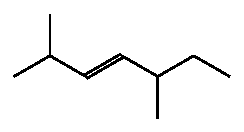
\includegraphics[max width=0.92\linewidth,max height=8.5cm]{qui/org_ej_nombre}
\end{center}
\alts{3,6-dimetilhept-4-eno}{2,5-dimetilheptano}{5-etil-2-metilhex-3-eno}{2,5-dimetilhept-3-eno}
\solucion{\textbf{Paso 1. ¿Qué nos piden?} El nombre IUPAC: cadena principal, numeración, ramificaciones y sufijo.

 

\textbf{Paso 2. Tipo de compuesto.} Solo C e H y una línea doble: es un \textbf{alqueno} (sufijo -eno).

 

\textbf{Paso 3. Cadena principal.} Busca la cadena más larga que contenga el doble enlace. Partiendo del extremo inferior izquierdo: 1 C, sube al vértice ramificado, baja, doble, sube, baja al otro vértice ramificado, y sigue por la derecha 2 C más. Son \textbf{7 C}: hept-. Las dos líneas que salen hacia arriba y hacia abajo de los vértices ramificados son metilos.

 

\textbf{Paso 4. Numeración.} Desde la izquierda, el doble enlace queda entre C3 y C4 \ensuremath{\rightarrow} localizador 3. Desde la derecha quedaría en 4. Gana la izquierda: \textbf{hept-3-eno}.

 

\textbf{Paso 5. Ramificaciones.} Con esa numeración, los metilos están en C2 y C5: \textbf{2,5-dimetil}.

 

\textbf{Respuesta:} 2,5-dimetilhept-3-eno.

 

\textbf{Comprobación:} el nombre indica $7 + 2 = 9$ C y el dibujo tiene 9 vértices y extremos. Fórmula: C\textsubscript{9}H\textsubscript{18} = C\textsubscript{n}H\textsubscript{2n}, como corresponde a un alqueno. \ding{52}

 

\textbf{¿Por qué no las otras?} "3,6-dimetilhept-4-eno" numera desde la derecha y le da al doble un número mayor (4 en vez de 3). "2,5-dimetilheptano" ignora el doble enlace (sería un alcano, C\textsubscript{9}H\textsubscript{20}). "5-etil-2-metilhex-3-eno" elige una cadena de 6 C cuando hay una de 7, y además deja una rama etilo que debería ser parte de la cadena.

\textbf{\color{cienciaD}Para recordar.} Cadena más larga con el doble enlace, numerada para que el doble tenga el número más bajo; luego las ramas en orden alfabético.}{D}
\end{elejemplo}

%% =====================================================================
%% qui_funcionales
\section[Grupos funcionales]{Grupos funcionales}
\modcomun\ \ {\color{gris}\itshape Haluros, alcoholes, fenoles, éteres, sulfuros, aldehídos, cetonas, ácidos carboxílicos, ésteres, anhídridos, amidas, aminas y nitrilos: cómo se escriben, cómo se nombran, cómo reconocerlos en fármacos y aromas, y para qué se usan.\par}
\subsection{¿Qué es un grupo funcional?}
Un \textbf{grupo funcional} es un átomo o grupo de átomos (casi siempre con O, N, S o un halógeno) que le da a la molécula sus propiedades químicas. Moléculas con el mismo grupo funcional se comportan de forma parecida.

 

Se escribe \textbf{R} para el resto de la molécula (la parte de C e H). Así, R--OH es "cualquier alcohol": CH\textsubscript{3}--OH, CH\textsubscript{3}--CH\textsubscript{2}--OH, etc.

 

Cuando una molécula tiene varios grupos, el de \textbf{mayor prioridad} da el sufijo del nombre y los demás se nombran como prefijos:

 
\begin{center}
\textbf{ácido carboxílico > anhídrido > éster > amida > nitrilo > aldehído > cetona > alcohol > amina > éter > haluro}
\end{center}
  
\begin{ejemplo}[{Ejemplo}] HO--CH\textsubscript{2}--CH\textsubscript{2}--CH\textsubscript{2}--COOH tiene un alcohol y un ácido. Manda el ácido: la cadena se numera desde el COOH (C1) y el OH queda en C4 como prefijo "hidroxi": \textbf{ácido 4-hidroxibutanoico}.\end{ejemplo}
 
\begin{ojo}[{Nombres comunes}] El temario acepta nombres IUPAC o comunes. Conviene saber los dos para los compuestos famosos: acetona = propanona, ácido acético = ácido etanoico, formaldehído = metanal, cloroformo = triclorometano.\end{ojo}
\subsection{Oxígeno con enlaces simples: alcoholes, fenoles y éteres}
\begin{center}
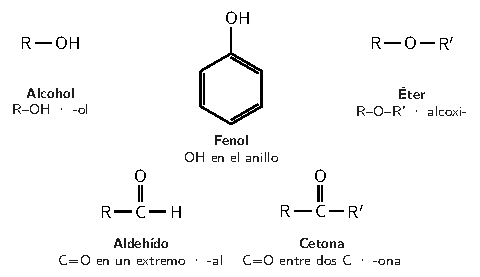
\includegraphics[max width=0.92\linewidth,max height=8.5cm]{qui/org_grupos_o}
\end{center}
  

\textbf{Alcohol, R--OH.} Sufijo \textbf{-ol}, con localizador: propan-2-ol. Ejemplos: metanol (tóxico), etanol (bebidas, alcohol gel, combustible), propan-2-ol (alcohol isopropílico, desinfectante), glicerol (cosméticos). Según el C que lleva el OH, son primarios (el C tiene 1 C vecino), secundarios (2) o terciarios (3). Forman \textbf{puentes de hidrógeno}: temperaturas de ebullición altas y los pequeños son solubles en agua.

 

\textbf{Fenol, OH unido a un anillo bencénico.} El fenol, C\textsubscript{6}H\textsubscript{5}OH, es desinfectante; los fenoles son antioxidantes y están en el timol del tomillo y en la vanilina. Son más ácidos que los alcoholes.

  

\textbf{Éter, R--O--R'.} El O está \textbf{entre dos carbonos}. IUPAC: el grupo pequeño con O se nombra "alcoxi": CH\textsubscript{3}--O--CH\textsubscript{2}--CH\textsubscript{3} es \textbf{metoxietano} (común: etil metil éter). El etoxietano (dietil éter) fue un anestésico y hoy es solvente. No forman puentes de hidrógeno entre sí: hierven a menor temperatura que el alcohol isómero.

 
\begin{ojo}[{Alcohol o fenol}] Si el OH está en un C del anillo bencénico, es fenol; si está en un C con solo enlaces simples, es alcohol.\end{ojo}
\subsection{El grupo carbonilo: aldehídos y cetonas}
El \textbf{carbonilo} es un C=O. Su posición define la familia:

 

\textbf{Aldehído, R--CHO.} El C=O está en un \textbf{extremo} de la cadena: el C lleva un H. Sufijo \textbf{-al}, sin número (el C del CHO siempre es C1): metanal, etanal, butanal. Ejemplos: metanal o formaldehído (la formalina conserva tejidos), benzaldehído (aroma de almendras), cinamaldehído (canela), vanilina (vainilla).

 

\textbf{Cetona, R--CO--R'.} El C=O está \textbf{entre dos carbonos}. Sufijo \textbf{-ona}, con localizador: pentan-2-ona, pentan-3-ona. La propanona (acetona) es el solvente del quitaesmalte; la butan-2-ona se usa en pinturas.

  
\begin{ejemplo}[{Ejemplo resuelto}] CH\textsubscript{3}--CH\textsubscript{2}--CH(CH\textsubscript{3})--CH\textsubscript{2}--CHO. \textbf{Paso 1.} Cadena más larga con el CHO: 5 C \ensuremath{\rightarrow} pentanal. \textbf{Paso 2.} El CHO es C1, así que el metilo queda en C3. \textbf{Nombre:} 3-metilpentanal. \textbf{Fórmula:} C\textsubscript{6}H\textsubscript{12}O.\end{ejemplo}
 
\begin{ojo}[{Error típico}] Llamar cetona a todo C=O. Mira los vecinos del carbono del C=O: si uno es H, es aldehído; si son dos C, es cetona; si uno es O o N, es ácido, éster o amida (siguiente sección).\end{ojo}
 
\begin{clave}[{Oxidación}] Alcohol primario \ensuremath{\rightarrow} aldehído \ensuremath{\rightarrow} ácido carboxílico. Alcohol secundario \ensuremath{\rightarrow} cetona.\end{clave}
\subsection{Ácidos carboxílicos y sus derivados: ésteres, anhídridos y amidas}
\begin{center}
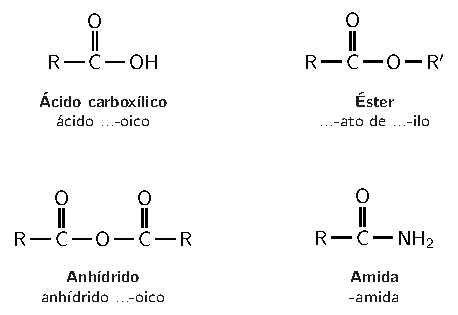
\includegraphics[max width=0.92\linewidth,max height=8.5cm]{qui/org_grupos_co}
\end{center}
  

\textbf{Ácido carboxílico, R--COOH.} "ácido \dots{}-oico": ácido metanoico (fórmico, de las hormigas), ácido etanoico (acético, del vinagre), ácido butanoico (mantequilla rancia). Son ácidos débiles y forman puentes de hidrógeno.

 

\textbf{Éster, R--COO--R'.} Se forma por \textbf{esterificación}: ácido + alcohol \ensuremath{\rightarrow} éster + agua. Nombre: la parte del ácido termina en \textbf{-ato} y la del alcohol en \textbf{-ilo}: CH\textsubscript{3}--COO--CH\textsubscript{2}--CH\textsubscript{3} es \textbf{etanoato de etilo} (acetato de etilo). Dan los \textbf{aromas frutales}: etanoato de 3-metilbutilo (plátano), butanoato de etilo (piña). Las grasas y aceites son ésteres.

  

\textbf{Anhídrido, R--CO--O--CO--R.} Dos grupos acilo unidos por un O (como dos ácidos que perdieron una molécula de agua). El anhídrido etanoico (acético) se usa para fabricar la aspirina.

 

\textbf{Amida, R--CO--NH\textsubscript{2}.} Sufijo \textbf{-amida}: etanamida. La urea es una amida; el \textbf{enlace peptídico} que une los aminoácidos en las proteínas es una amida, igual que el nailon y el paracetamol.

 
\begin{ojo}[{Éster o éter}] Los dos tienen C--O--C, pero el éster tiene además un C=O pegado a ese O. Sin C=O, es éter.\end{ojo}
\subsection{Nitrógeno, azufre y halógenos: aminas, nitrilos, sulfuros y haluros}
\begin{center}
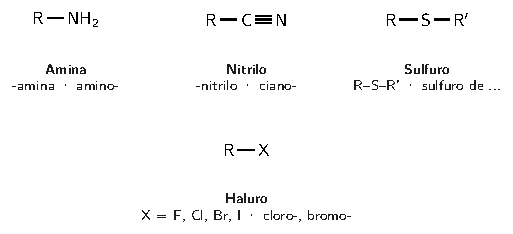
\includegraphics[max width=0.92\linewidth,max height=8.5cm]{qui/org_grupos_nsx}
\end{center}
  

\textbf{Amina, R--NH\textsubscript{2}} (también R\textsubscript{2}NH y R\textsubscript{3}N). Sufijo \textbf{-amina}: metanamina (metilamina). Son \textbf{básicas} y las pequeñas huelen a pescado. Están en los aminoácidos, la adrenalina, la anilina (colorantes) y alcaloides como la cafeína y la nicotina.

 

\textbf{Nitrilo, R--C\ensuremath{\equiv}N.} Sufijo \textbf{-nitrilo}, contando el C del CN: CH\textsubscript{3}--CN es etanonitrilo (acetonitrilo, un solvente). El propenonitrilo (acrilonitrilo) se usa para fibras acrílicas.

  

\textbf{Sulfuro (tioéter), R--S--R'.} Como un éter, pero con S: CH\textsubscript{3}--S--CH\textsubscript{3} es el sulfuro de dimetilo (olor a mar y a repollo cocido). El sulfuro de dialilo da parte del olor del ajo. No confundir con los tioles (R--SH), que se agregan al gas para detectar fugas.

 

\textbf{Haluro de alquilo, R--X} (X = F, Cl, Br, I). Se nombran con prefijos: clorometano, 2-bromopropano. El triclorometano (cloroformo) fue anestésico y hoy es solvente; los CFC dañan la capa de ozono; el PVC y el teflón son polímeros halogenados.
\subsection{Reconocer grupos en moléculas reales}
\begin{center}
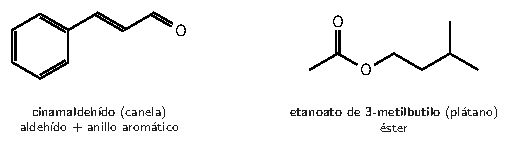
\includegraphics[max width=0.92\linewidth,max height=8.5cm]{qui/org_reales}
\end{center}
  

En la PAES aparecen fármacos, aromas e insecticidas dibujados en fórmula topológica. Para reconocer sus grupos, mira cada heteroátomo (O, N, S, halógeno) y a sus \textbf{vecinos}:

 
\begin{center}\small
\begin{tabular}{@{}ll@{}}
\toprule
\textbf{Lo que ves} & \textbf{Grupo} \\
\midrule
OH en C con solo simples & alcohol \\
OH en el anillo bencénico & fenol \\
C--O--C, sin C=O al lado & éter \\
C=O en un extremo (con H) & aldehído \\
C=O entre dos C & cetona \\
C=O con OH en el mismo C & ácido carboxílico \\
C=O con O--C en el mismo C & éster \\
C=O con N en el mismo C & amida \\
N con solo enlaces simples a C o H & amina \\
C\ensuremath{\equiv}N & nitrilo \\
\bottomrule
\end{tabular}
\end{center}
  
\begin{ejemplo}[{Ejemplo resuelto: paracetamol}] HO--C\textsubscript{6}H\textsubscript{4}--NH--CO--CH\textsubscript{3}. \textbf{Paso 1.} El OH está sobre el anillo: \textbf{fenol}. \textbf{Paso 2.} El N está unido a un C que tiene un C=O: no es amina, es \textbf{amida}. \textbf{Paso 3.} No hay ácido ni éster: el único C=O es parte de la amida.\end{ejemplo}
 
\begin{ojo}[{Error típico}] Mirar un átomo solo. Un O puede ser alcohol, éter, cetona, éster o ácido según sus vecinos, y un N puede ser amina o amida. Revisa siempre el carbono de al lado.\end{ojo}
\subsection{Lo clave del tema}
\begin{center}\small
\begin{tabularx}{\linewidth}{@{}>{\raggedright\arraybackslash\hsize=0.72\hsize}X>{\raggedright\arraybackslash\hsize=0.60\hsize}X>{\raggedright\arraybackslash\hsize=1.15\hsize}X>{\raggedright\arraybackslash\hsize=1.53\hsize}X@{}}
\toprule
\textbf{Grupo} & \textbf{Fórmula} & \textbf{Nombre (ejemplo)} & \textbf{Uso o característica} \\
\midrule
Haluro & R--X & triclorometano (cloroformo) & solventes, CFC, PVC \\
Alcohol & R--OH & etanol & bebidas, desinfectante; puentes de H \\
Fenol & Ar--OH & fenol & desinfectante, antioxidante \\
Éter & R--O--R' & etoxietano (dietil éter) & anestésico antiguo, solvente \\
Sulfuro & R--S--R' & sulfuro de dimetilo & olores (ajo, mar) \\
Aldehído & R--CHO & metanal (formaldehído) & conservante (formalina), aromas \\
Cetona & R--CO--R' & propanona (acetona) & solvente, quitaesmalte \\
Ácido carboxílico & R--COOH & ácido etanoico (acético) & vinagre; ácido débil \\
Éster & R--COO--R' & etanoato de etilo & aromas frutales, grasas \\
Anhídrido & R--CO--O--CO--R & anhídrido etanoico & síntesis de aspirina \\
Amida & R--CO--NH\textsubscript{2} & etanamida & proteínas, nailon, paracetamol \\
Amina & R--NH\textsubscript{2} & metanamina (metilamina) & básicas, olor a pescado, alcaloides \\
Nitrilo & R--C\ensuremath{\equiv}N & etanonitrilo (acetonitrilo) & solventes, fibras acrílicas \\
\bottomrule
\end{tabularx}
\end{center}
  
\begin{clave}[{Recuerda}] · En un C=O mira los vecinos: H (aldehído), 2 C (cetona), OH (ácido), O--C (éster), N (amida).\par · N--C=O es una amida.\par · Etanoato de propilo y propanoato de etilo son distintos: "-ato" es la parte del ácido (con el C=O) y "-ilo" la del alcohol.\end{clave}
  
\begin{clave}[{Método PAES}] 1. Encierra cada heteroátomo. 2. Mira sus vecinos y usa la tabla de la sección anterior. 3. Si te piden el nombre, busca el grupo de mayor prioridad: da el sufijo y fija la numeración (C1 en el CHO o el COOH). 4. Si te piden un uso, asocia: éster--aroma, amida--proteínas, cetona--acetona, ácido--vinagre, amina--olor a pescado.\end{clave}
\begin{elejemplo}{PAES Regular 2026, adaptada}
El ácido acetilsalicílico (aspirina) es uno de los analgésicos más usados del mundo. Su estructura es la siguiente:

¿Cuáles grupos funcionales están presentes en esta molécula, además del anillo aromático?
\begin{center}
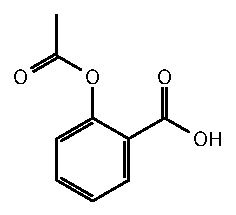
\includegraphics[max width=0.92\linewidth,max height=8.5cm]{qui/org_aspirina}
\end{center}
\alts{Cetona y éter}{Ácido carboxílico y éster}{Aldehído y alcohol}{Ácido carboxílico y cetona}
\solucion{\textbf{Paso 1. ¿Qué nos piden?} Nombrar los grupos funcionales que se ven en la estructura.

 

\textbf{Paso 2. Encierra los heteroátomos.} Hay 4 O, en dos grupos: uno a la derecha (C=O y OH) y otro arriba a la izquierda (un O unido al anillo y un C=O).

 

\textbf{Paso 3. Grupo de la derecha.} Un carbono tiene un C=O y un OH a la vez: es un \textbf{ácido carboxílico} (--COOH).

 

\textbf{Paso 4. Grupo de arriba.} El O unido al anillo está unido, del otro lado, a un C que tiene un C=O (y un CH\textsubscript{3}). Un O entre dos C, con C=O al lado: es un \textbf{éster} (--O--CO--CH\textsubscript{3}). No es éter, porque hay un C=O pegado; no es cetona, porque el C del C=O está unido a un O.

 

\textbf{Respuesta:} ácido carboxílico y éster.

 

\textbf{Comprobación:} la aspirina se fabrica haciendo reaccionar el ácido salicílico (que tiene un fenol) con anhídrido etanoico: el OH del fenol se convierte en el éster. Su fórmula es C\textsubscript{9}H\textsubscript{8}O\textsubscript{4}: los 4 O son los 2 del ácido y los 2 del éster. \ding{52}

 

\textbf{¿Por qué no las otras?} "Cetona y éter" mira el C=O y el C--O--C por separado, sin notar que están unidos: juntos son un éster. "Aldehído y alcohol" confunde el COOH con un CHO más un OH. "Ácido carboxílico y cetona" acierta el ácido, pero el otro C=O no está entre dos C: tiene un O al lado.

\textbf{\color{cienciaD}Para recordar.} Antes de nombrar un C=O o un O, mira a sus vecinos: juntos pueden formar un grupo distinto.}{B}
\end{elejemplo}

\chapter{Reacciones químicas y estequiometría}
%% =====================================================================
%% qui_leyes
\section[Leyes ponderales y balance de ecuaciones]{Leyes ponderales y balance de ecuaciones}
\modcomun\ \ {\color{gris}\itshape Las partes de una ecuación química, la conservación de la masa (Lavoisier), las proporciones definidas (Proust) y múltiples (Dalton), y cómo balancear una ecuación por tanteo.\par}
\subsection{Las partes de una ecuación química}
Una \textbf{reacción química} es un proceso en el que unas sustancias se transforman en otras distintas. Se escribe con una \textbf{ecuación química}:

 
\begin{center}
CH\textsubscript{4} (g) + 2 O\textsubscript{2} (g) \ensuremath{\rightarrow} CO\textsubscript{2} (g) + 2 H\textsubscript{2}O (l)
\end{center}
 

Se lee: «un metano gaseoso reacciona con dos oxígenos gaseosos y forma un dióxido de carbono gaseoso y dos aguas líquidas».

 
\begin{center}\small
\begin{tabularx}{\linewidth}{@{}>{\raggedright\arraybackslash\hsize=0.63\hsize}X>{\raggedright\arraybackslash\hsize=1.79\hsize}X>{\raggedright\arraybackslash\hsize=0.58\hsize}X@{}}
\toprule
\textbf{Parte} & \textbf{Qué es} & \textbf{En el ejemplo} \\
\midrule
Reactantes & lo que hay al comienzo, a la izquierda & CH\textsubscript{4} y O\textsubscript{2} \\
Productos & lo que se forma, a la derecha & CO\textsubscript{2} y H\textsubscript{2}O \\
Flecha & «reacciona y forma» & \ensuremath{\rightarrow} \\
Coeficiente & número \textbf{delante} de la fórmula: cuántas moléculas (o mol) & el 2 de 2 O\textsubscript{2} \\
Subíndice & número \textbf{pequeño abajo}: cuántos átomos hay en una molécula & el 4 de CH\textsubscript{4} \\
Estado & (s) sólido, (l) líquido, (g) gas, (ac) acuoso, disuelto en agua & (g), (l) \\
\bottomrule
\end{tabularx}
\end{center}
  
\begin{clave}[{Coeficiente por subíndice}] Para contar átomos, multiplica el coeficiente por el subíndice. En 2 H\textsubscript{2}O hay 2 moléculas de agua: $2\cdot 2 = 4$ átomos de H y $2\cdot 1 = 2$ átomos de O.\end{clave}
 
\begin{clave}[{Con paréntesis}] En 3 Ca(OH)\textsubscript{2} el 2 multiplica a todo el paréntesis: por fórmula hay 1 Ca, 2 O y 2 H. Con el coeficiente: 3 Ca, 6 O y 6 H.\end{clave}
 
\begin{ojo}[{Error típico}] Creer que el subíndice y el coeficiente significan lo mismo. 2 O (dos átomos de oxígeno sueltos) no es lo mismo que O\textsubscript{2} (una molécula de oxígeno), ni que 2 O\textsubscript{2} (dos moléculas, cuatro átomos).\end{ojo}
\subsection{Ley de conservación de la masa (Lavoisier)}
Antoine Lavoisier (siglo XVIII) masó con cuidado los reactantes y los productos de muchas reacciones hechas en recipientes cerrados y llegó a esta ley:

 
\begin{clave}[{Ley de Lavoisier}] En una reacción química, la masa total de los reactantes es igual a la masa total de los productos. La materia no se crea ni se destruye: se transforma.\end{clave}
 

\textbf{¿Por qué se cumple?} Mira el diagrama de partículas de 2 H\textsubscript{2} + O\textsubscript{2} \ensuremath{\rightarrow} 2 H\textsubscript{2}O. Los átomos solo se \textbf{reordenan}: se rompen unos enlaces y se forman otros, pero antes y después hay los mismos átomos (8 de H y 4 de O). Si los átomos son los mismos, la masa también.

 
\begin{center}
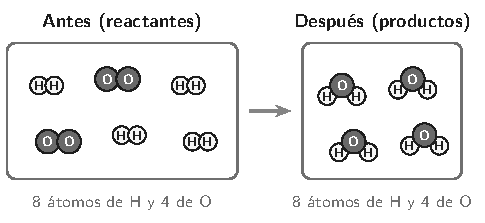
\includegraphics[max width=0.92\linewidth,max height=8.5cm]{qui/reac_particulas}
\end{center}
  
\begin{ejemplo}[{Ejemplo resuelto}] En un recipiente cerrado reaccionan completamente 12 g de magnesio con 8 g de oxígeno y se forma óxido de magnesio. ¿Qué masa de óxido se forma?\par \textbf{Paso 1.} Todo reaccionó: la masa de los reactantes es $12 + 8 = 20$ g.\par \textbf{Paso 2.} Por Lavoisier, la masa del producto es la misma: \textbf{20 g} de óxido de magnesio.\end{ejemplo}
 
\begin{clave}[{Si algo sobra}] Si en un recipiente cerrado pones 12 g de Mg y 10 g de O\textsubscript{2}, y se forman 20 g de óxido, la masa total sigue siendo $12 + 10 = 22$ g: son 20 g de óxido más $22 - 20 = 2$ g de oxígeno que \textbf{sobró} sin reaccionar.\end{clave}
 
\begin{ojo}[{Ojo}] Se conserva la \textbf{masa} y se conservan los \textbf{átomos}, pero no necesariamente el número de moléculas: en el diagrama hay 6 moléculas antes y 4 después.\end{ojo}
\subsection{Sistema abierto y sistema cerrado}
Cuando mezclas vinagre con bicarbonato se forma un gas, CO\textsubscript{2}. Si haces la reacción sobre una balanza, el resultado depende del recipiente:

 
\begin{center}
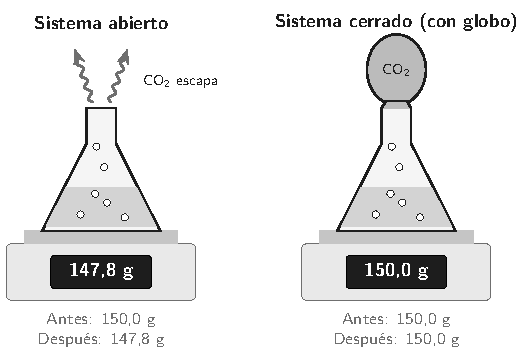
\includegraphics[max width=0.92\linewidth,max height=8.5cm]{qui/reac_balanza}
\end{center}
 

\textbf{Sistema abierto.} El CO\textsubscript{2} escapa al aire y la balanza ya no lo masa: marca 2,2 g menos. Esos 2,2 g son justamente el CO\textsubscript{2} que salió.

 

\textbf{Sistema cerrado.} El globo atrapa el gas. Nada entra ni sale y la balanza marca lo mismo antes y después.

  
\begin{ojo}[{Error típico}] Decir que en el sistema abierto «no se cumple la ley de Lavoisier». Sí se cumple: la masa no desapareció, se fue como gas. Para comprobar la ley hay que trabajar en un sistema cerrado o medir también el gas.\end{ojo}
 
\begin{ejemplo}[{Ejemplo resuelto}] Se calientan 10 g de carbonato de calcio en un crisol abierto: CaCO\textsubscript{3} (s) \ensuremath{\rightarrow} CaO (s) + CO\textsubscript{2} (g). Al final quedan 5,6 g de sólido (CaO). ¿Qué masa de CO\textsubscript{2} se liberó?\par \textbf{Paso 1.} Por Lavoisier: masa de CaCO\textsubscript{3} = masa de CaO + masa de CO\textsubscript{2}.\par \textbf{Paso 2.} $10 = 5{,}6 + m$, así que $m = 10 - 5{,}6 = 4{,}4$ g de CO\textsubscript{2}.\end{ejemplo}
 
\begin{clave}[{Al revés también pasa}] Si un metal se oxida en un recipiente abierto, el sólido \textbf{gana} masa: incorpora oxígeno del aire, que antes no estaba sobre la balanza.\end{clave}
\subsection{Ley de las proporciones definidas (Proust)}
\begin{clave}[{Ley de Proust}] Un compuesto siempre está formado por los mismos elementos combinados en la misma proporción en masa, sin importar cómo se obtuvo ni de dónde viene.\end{clave}
 

El agua pura siempre tiene 1 g de hidrógeno por cada 8 g de oxígeno (proporción en masa 1 : 8), sea de lluvia, de un río o hecha en el laboratorio.

 

\textbf{Consecuencia:} si mezclas los elementos en otra proporción, la reacción no cambia de proporción: uno de ellos \textbf{sobra} (queda en exceso).

 
\begin{center}\small
\begin{tabular}{@{}llll@{}}
\toprule
\textbf{Mg (g)} & \textbf{O (g)} & \textbf{Óxido formado (g)} & \textbf{Sobra} \\
\midrule
3 & 2 & 5 & nada \\
6 & 4 & 10 & nada \\
6 & 5 & 10 & 1 g de O \\
9 & 4 & 10 & 3 g de Mg \\
\bottomrule
\end{tabular}
\end{center}
  
\begin{ejemplo}[{Ejemplo resuelto}] El magnesio y el oxígeno se combinan en proporción 3 : 2. ¿Qué pasa si mezclas 9 g de Mg con 4 g de O?\par \textbf{Paso 1.} Para 4 g de O hacen falta $4\cdot\dfrac{3}{2} = 6$ g de Mg. Hay 9 g: alcanza y sobra.\par \textbf{Paso 2.} Reaccionan 6 g de Mg con 4 g de O y se forman $6 + 4 = 10$ g de óxido.\par \textbf{Paso 3.} Sobran $9 - 6 = 3$ g de Mg.\par \textbf{Comprobación:} masa inicial $9 + 4 = 13$ g; masa final $10 + 3 = 13$ g. \ding{52}\end{ejemplo}
 
\begin{ojo}[{Error típico}] Sumar todo lo que pusiste para obtener la masa del producto. Solo se suma lo que \textbf{reaccionó}; lo que sobra no forma producto.\end{ojo}
 
\begin{clave}[{En un gráfico}] Si graficas la masa de un elemento contra la masa del otro que se combina con él, obtienes una \textbf{recta que pasa por el origen}: la razón entre las masas es siempre la misma.\end{clave}
\subsection{Ley de las proporciones múltiples (Dalton)}
A veces dos elementos forman \textbf{más de un compuesto}. El carbono y el oxígeno forman CO y CO\textsubscript{2}; el azufre y el oxígeno forman SO\textsubscript{2} y SO\textsubscript{3}.

 
\begin{clave}[{Ley de Dalton}] Si dos elementos forman varios compuestos, las masas de uno de ellos que se combinan con una \textbf{misma masa} del otro están en una razón de números enteros sencillos.\end{clave}
 

\textbf{Cómo se aplica.} Fija la masa de un elemento y compara las masas del otro.

 
\begin{center}\small
\begin{tabular}{@{}lll@{}}
\toprule
\textbf{Compuesto} & \textbf{Masa de C (g)} & \textbf{Masa de O (g)} \\
\midrule
CO & 12 & 16 \\
CO\textsubscript{2} & 12 & 32 \\
\bottomrule
\end{tabular}
\end{center}
 

Con los mismos 12 g de C, las masas de O son 16 g y 32 g: razón $16 : 32 = 1 : 2$, números enteros sencillos.

  
\begin{ejemplo}[{Ejemplo resuelto}] En SO\textsubscript{2} hay 32 g de S por cada 32 g de O, y en SO\textsubscript{3} hay 32 g de S por cada 48 g de O. Con la misma masa de S, las masas de O están en razón $32 : 48 = 2 : 3$. \ding{52} Se cumple la ley.\end{ejemplo}
 
\begin{ojo}[{Ojo con los porcentajes}] Cada compuesto tiene su propio porcentaje fijo (Proust), pero compuestos distintos de los mismos elementos tienen porcentajes distintos. En CO hay $\dfrac{12}{28}\approx 43\%$ de C y en CO\textsubscript{2}, $\dfrac{12}{44}\approx 27\%$. Si en dos experimentos con hierro y oxígeno el porcentaje de hierro es distinto, se formaron dos óxidos distintos.\end{ojo}
 
\begin{clave}[{Las tres leyes juntas}] Las leyes ponderales llevaron a Dalton a su teoría atómica: los átomos se combinan en números enteros, se reordenan en las reacciones y no se crean ni se destruyen.\end{clave}
\subsection{Balancear una ecuación}
\textbf{Balancear} es elegir los coeficientes para que haya el mismo número de átomos de cada elemento a los dos lados. Así la ecuación cumple la ley de Lavoisier.

 

\textbf{Ejemplo:} C\textsubscript{3}H\textsubscript{8} + O\textsubscript{2} \ensuremath{\rightarrow} CO\textsubscript{2} + H\textsubscript{2}O.

 

\textbf{Paso 1. Carbono.} Hay 3 C a la izquierda: pon 3 delante del CO\textsubscript{2}.

 

\textbf{Paso 2. Hidrógeno.} Hay 8 H a la izquierda; cada agua tiene 2: pon 4 delante del H\textsubscript{2}O.

 

\textbf{Paso 3. Oxígeno, al final.} A la derecha hay $3\cdot 2 + 4\cdot 1 = 10$ átomos de O; cada O\textsubscript{2} tiene 2: pon 5 delante del O\textsubscript{2}.

 

\textbf{Resultado:} C\textsubscript{3}H\textsubscript{8} + 5 O\textsubscript{2} \ensuremath{\rightarrow} 3 CO\textsubscript{2} + 4 H\textsubscript{2}O.

 
\begin{center}\small
\begin{tabular}{@{}lll@{}}
\toprule
\textbf{Átomo} & \textbf{Izquierda} & \textbf{Derecha} \\
\midrule
C & 3 & 3 \\
H & 8 & $4\cdot 2 = 8$ \\
O & $5\cdot 2 = 10$ & $6 + 4 = 10$ \\
\bottomrule
\end{tabular}
\end{center}
  
\begin{clave}[{Orden práctico}] 1. Metales. 2. No metales distintos de H y O. 3. Hidrógeno. 4. Oxígeno al final. Si un grupo como NO\textsubscript{3} o SO\textsubscript{4} pasa entero de un lado al otro, cuéntalo como un bloque.\end{clave}
 
\begin{clave}[{Con número impar}] Al + O\textsubscript{2} \ensuremath{\rightarrow} Al\textsubscript{2}O\textsubscript{3}. Para tener O par a los dos lados, pon 2 Al\textsubscript{2}O\textsubscript{3} (6 O): necesitas 3 O\textsubscript{2}. Luego hay 4 Al a la derecha: 4 Al. Queda 4 Al + 3 O\textsubscript{2} \ensuremath{\rightarrow} 2 Al\textsubscript{2}O\textsubscript{3}.\end{clave}
 
\begin{ojo}[{Nunca cambies un subíndice}] Cambiar H\textsubscript{2}O por H\textsubscript{2}O\textsubscript{2} «para que cuadre» cambia la sustancia: el agua oxigenada no es agua. Solo se cambian los coeficientes, y se usan los enteros más pequeños posibles.\end{ojo}
\subsection{Lo clave del tema}
\begin{center}\small
\begin{tabularx}{\linewidth}{@{}>{\raggedright\arraybackslash\hsize=0.39\hsize}X>{\raggedright\arraybackslash\hsize=1.30\hsize}X>{\raggedright\arraybackslash\hsize=1.30\hsize}X@{}}
\toprule
\textbf{Ley o idea} & \textbf{Qué dice} & \textbf{Cómo se usa} \\
\midrule
Lavoisier & masa de reactantes = masa de productos & resta para hallar la masa que falta o la que sobró \\
Proust & cada compuesto tiene una proporción en masa fija & regla de tres con la proporción; lo que no calza, sobra \\
Dalton & con una masa fija de un elemento, las masas del otro están en razón entera & fija un elemento y divide las masas del otro \\
Balance & mismos átomos a ambos lados & cambia coeficientes, nunca subíndices \\
\bottomrule
\end{tabularx}
\end{center}
 
\begin{clave}[{Recuerda}] · Lo que sobra no forma producto: con 9 g de Mg y 4 g de O reaccionan 6 g + 4 g, se forman 10 g de óxido y sobran 3 g de Mg.\par · Si en un sistema abierto la masa baja, la que falta es el gas que escapó: Lavoisier se cumple.\par · En 2 H\textsubscript{2}O hay $2\cdot 2 = 4$ H.\par · Se balancea con coeficientes, nunca con subíndices: 2 H\textsubscript{2} + O\textsubscript{2} \ensuremath{\rightarrow} 2 H\textsubscript{2}O.\par · En los diagramas de partículas, escribe las moléculas tal como aparecen (X\textsubscript{2}) y no cuentes las que sobran.\end{clave}
 
\begin{clave}[{Método PAES}] 1. Escribe qué reacciona y qué se forma. 2. Si hay masas, usa Lavoisier (suma o resta) y Proust (proporción fija). 3. Si hay coeficientes, cuenta átomos elemento por elemento con una tabla izquierda/derecha. 4. En un diagrama, cuenta moléculas antes y después, descuenta las que sobran y simplifica. 5. Comprueba que la masa total, o los átomos, sean iguales a ambos lados.\end{clave}
\begin{elejemplo}{PAES Invierno 2026, adaptada}
Dos sustancias, X e Y, reaccionan para formar un único compuesto Z. Se realizaron tres ensayos y se registraron las masas iniciales de X e Y, la masa final de Z y el reactivo que quedó en exceso:
\begin{center}\small
\begin{tabular}{@{}lllll@{}}
\toprule
\textbf{Ensayo} & \textbf{Masa de X (g)} & \textbf{Masa de Y (g)} & \textbf{Masa de Z (g)} & \textbf{Exceso} \\
\midrule
\textbf{1} & 14 & 4 & 18 & nada \\
\textbf{2} & 7 & 4 & 9 & 2 g de Y \\
\textbf{3} & 20 & 4 & 18 & 6 g de X \\
\bottomrule
\end{tabular}
\end{center}
\altslargas{En los tres ensayos, la suma de las masas iniciales de X e Y es igual a la masa final de Z.}{7 g de X reaccionan exactamente con 4 g de Y.}{Para formar Z, las sustancias X e Y se combinan en una proporción en masa de 7 : 2.}{20 g de X reaccionan exactamente con 4 g de Y.}
\solucion{\textbf{Paso 1. ¿Qué nos piden?} La afirmación correcta sobre cómo se combinan X e Y. La clave es el ensayo en que no sobra nada: ahí todo lo que se puso reaccionó.

\textbf{Paso 2. Ensayo 1, sin exceso.} Reaccionaron 14 g de X con 4 g de Y y se formaron $14 + 4 = 18$ g de Z. \ding{52} Se cumple Lavoisier.

\textbf{Paso 3. La proporción.} $14 : 4$. Dividimos ambos por 2: $7 : 2$. Por cada 7 g de X reaccionan 2 g de Y.

\textbf{Paso 4. Revisa el ensayo 2 con la proporción.} Hay 7 g de X: necesitan 2 g de Y. Se pusieron 4 g, así que sobran $4 - 2 = 2$ g de Y y se forman $7 + 2 = 9$ g de Z. Coincide con la tabla. \ding{52}

\textbf{Paso 5. Revisa el ensayo 3.} Hay 4 g de Y: necesitan 14 g de X. Se pusieron 20 g, así que sobran $20 - 14 = 6$ g de X y se forman 18 g de Z. Coincide. \ding{52}

\textbf{Respuesta:} X e Y se combinan en proporción en masa 7 : 2 (ley de Proust).

\textbf{Comprobación:} en cada ensayo, masa inicial = masa de Z + exceso. Ensayo 2: $7 + 4 = 11$ y $9 + 2 = 11$. Ensayo 3: $20 + 4 = 24$ y $18 + 6 = 24$. \ding{52} La masa total se conserva, contando lo que sobró.

\textbf{¿Por qué no las otras?} La primera olvida el exceso: en el ensayo 2, $7 + 4 = 11$ g, pero solo se forman 9 g de Z porque sobran 2 g de Y. La segunda lee el ensayo 2 como si todo reaccionara, pero ahí sobró Y: 7 g de X reaccionan con 2 g de Y, no con 4. La cuarta lee el ensayo 3 sin descontar el exceso: de los 20 g de X solo reaccionaron 14.

\textbf{\color{cienciaD}Para recordar.} La proporción de combinación se lee en el ensayo donde no sobra nada; en los demás, masa inicial = producto + exceso.}{C}
\end{elejemplo}

%% =====================================================================
%% qui_mol
\section[El mol y la masa molar]{El mol y la masa molar}
\modcomun\ \ {\color{gris}\itshape Qué es un mol y el número de Avogadro, cómo calcular una masa molar, y cómo pasar de masa a cantidad de sustancia, a número de moléculas y a número de átomos.\par}
\subsection{Contar por montones: el mol}
Los átomos y las moléculas son tan pequeños que en una gota de agua hay miles de trillones. Para no trabajar con números gigantes, los químicos cuentan por «montones», igual que contamos huevos por docena.

 
\begin{clave}[{El mol}] Un \textbf{mol} es la cantidad de sustancia que contiene $6{,}02\cdot 10^{23}$ partículas. Ese número se llama \textbf{número de Avogadro}, $N_A$.\end{clave}
 

Una docena son 12 cosas, sean huevos o lápices. Un mol son $6{,}02\cdot 10^{23}$ partículas, sean átomos, moléculas o iones:

 
\begin{itemize}
  \item 1 mol de átomos de Fe = $6{,}02\cdot 10^{23}$ átomos de Fe.
  \item 1 mol de moléculas de H\textsubscript{2}O = $6{,}02\cdot 10^{23}$ moléculas de agua.
  \item 2 mol de CO\textsubscript{2} = $2\cdot 6{,}02\cdot 10^{23} = 1{,}204\cdot 10^{24}$ moléculas.
\end{itemize}
  
\begin{clave}[{Nombre y unidad}] La magnitud se llama \textbf{cantidad de sustancia}, se simboliza $n$ y su unidad es el \textbf{mol}. Es una de las unidades básicas del Sistema Internacional.\end{clave}
 
\begin{clave}[{Mitades y dobles}] $0{,}5$ mol son $3{,}01\cdot 10^{23}$ partículas; $1{,}5$ mol son $9{,}03\cdot 10^{23}$; $3$ mol son $1{,}806\cdot 10^{24}$. En la PAES los números se eligen para que estas cuentas salgan sin calculadora.\end{clave}
 
\begin{ojo}[{Error típico}] Pensar que un mol de cualquier sustancia tiene la misma masa. Un mol de huevos y un mol de sandías tienen el mismo número de unidades, pero no pesan lo mismo. Lo mismo pasa con un mol de H\textsubscript{2} y un mol de CO\textsubscript{2}.\end{ojo}
\subsection{Masa atómica y masa molar}
La \textbf{masa molar} ($M$) es la masa de un mol de una sustancia, en g/mol. Se calcula sumando las masas atómicas de todos los átomos de la fórmula (la PAES las entrega en la tabla periódica o en el enunciado).

 

\textbf{Ejemplo: agua, H\textsubscript{2}O.} 2 H y 1 O: $M = 2\cdot 1 + 16 = 18$ g/mol.

 

\textbf{Ejemplo: carbonato de calcio, CaCO\textsubscript{3}.} 1 Ca, 1 C y 3 O: $M = 40 + 12 + 3\cdot 16 = 100$ g/mol.

 

\textbf{Ejemplo: glucosa, C\textsubscript{6}H\textsubscript{12}O\textsubscript{6}.} $M = 6\cdot 12 + 12\cdot 1 + 6\cdot 16 = 72 + 12 + 96 = 180$ g/mol.

 
\begin{center}\small
\begin{tabular}{@{}lll@{}}
\toprule
\textbf{Sustancia} & \textbf{Cuenta} & \textbf{$M$ (g/mol)} \\
\midrule
O\textsubscript{2} & $2\cdot 16$ & 32 \\
CO\textsubscript{2} & $12 + 2\cdot 16$ & 44 \\
NH\textsubscript{3} & $14 + 3\cdot 1$ & 17 \\
NaCl & $23 + 35{,}5$ & 58,5 \\
H\textsubscript{2}SO\textsubscript{4} & $2 + 32 + 64$ & 98 \\
\bottomrule
\end{tabular}
\end{center}
  
\begin{clave}[{Con paréntesis}] Ca(OH)\textsubscript{2} tiene 1 Ca, 2 O y 2 H: $M = 40 + 2\cdot 16 + 2\cdot 1 = 74$ g/mol.\end{clave}
 
\begin{ojo}[{Error típico}] Olvidar el subíndice del paréntesis: $40 + 16 + 1 = 57$ g/mol para Ca(OH)\textsubscript{2} está mal. El 2 multiplica al O y al H.\end{ojo}
 
\begin{ojo}[{Fórmulas condensadas}] En CH\textsubscript{3}OH hay que juntar todos los H: $3 + 1 = 4$. $M = 12 + 4\cdot 1 + 16 = 32$ g/mol. Contar solo los 3 del CH\textsubscript{3} es un error frecuente.\end{ojo}
 
\begin{clave}[{Más átomos no es más masa}] El CH\textsubscript{4} tiene 5 átomos y $M = 16$ g/mol; el HCl tiene 2 átomos y $M = 36{,}5$ g/mol. Lo que manda es la masa de cada átomo, no cuántos hay.\end{clave}
\subsection{De masa a mol y de mol a masa}
\begin{center}
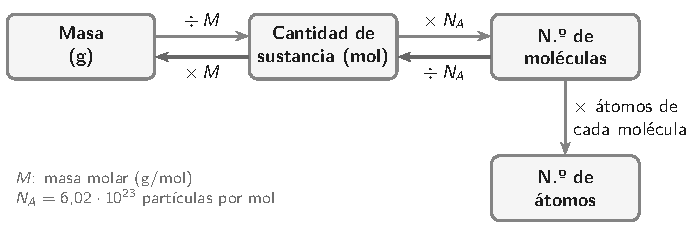
\includegraphics[max width=0.92\linewidth,max height=8.5cm]{qui/reac_mapa_mol}
\end{center}
 

La masa molar es el puente entre lo que se mide en la balanza (gramos) y lo que se cuenta (mol):

 
\begin{center}
$n = \dfrac{m}{M}$ y $m = n\cdot M$
\end{center}
  
\begin{ejemplo}[{Ejemplo resuelto 1}] ¿Cuántos mol hay en 88 g de CO\textsubscript{2}? ($M = 44$ g/mol)\par $n = \dfrac{88}{44} = 2$ mol.\end{ejemplo}
 
\begin{ejemplo}[{Ejemplo resuelto 2}] ¿Qué masa tienen 0,5 mol de glucosa? ($M = 180$ g/mol)\par $m = 0{,}5\cdot 180 = 90$ g.\end{ejemplo}
 
\begin{ejemplo}[{Ejemplo resuelto 3}] ¿Cuántos mol hay en 4,9 g de H\textsubscript{2}SO\textsubscript{4}? ($M = 98$ g/mol)\par $n = \dfrac{4{,}9}{98} = 0{,}05$ mol.\end{ejemplo}
 
\begin{ojo}[{Revisa las unidades}] g ÷ (g/mol) = mol. Si te queda «mol²/g» o «g²/mol», dividiste al revés. Un control rápido: si la masa es menor que $M$, tienes menos de 1 mol.\end{ojo}
\subsection{Moléculas y átomos dentro de las moléculas}
Para contar partículas se multiplica por el número de Avogadro: $N = n\cdot N_A$.

 

Pero cuidado: una molécula tiene varios átomos. En 2 mol de H\textsubscript{2}O:

 
\begin{center}\small
\begin{tabular}{@{}lll@{}}
\toprule
\textbf{Qué se cuenta} & \textbf{mol} & \textbf{Número} \\
\midrule
moléculas de H\textsubscript{2}O & 2 & $1{,}204\cdot 10^{24}$ \\
átomos de H & $2\cdot 2 = 4$ & $2{,}408\cdot 10^{24}$ \\
átomos de O & $2\cdot 1 = 2$ & $1{,}204\cdot 10^{24}$ \\
átomos en total & $2\cdot 3 = 6$ & $3{,}612\cdot 10^{24}$ \\
\bottomrule
\end{tabular}
\end{center}
  
\begin{ejemplo}[{Ejemplo resuelto}] ¿Cuántos átomos de hidrógeno hay en 8 g de metano, CH\textsubscript{4}? ($M = 16$ g/mol)\par \textbf{Paso 1.} Mol de CH\textsubscript{4}: $\dfrac{8}{16} = 0{,}5$ mol.\par \textbf{Paso 2.} Cada molécula tiene 4 H: $0{,}5\cdot 4 = 2$ mol de átomos de H.\par \textbf{Paso 3.} $2\cdot 6{,}02\cdot 10^{23} = 1{,}204\cdot 10^{24}$ átomos de H.\end{ejemplo}
 
\begin{ojo}[{Error típico}] Responder el número de \textbf{moléculas} cuando preguntan por \textbf{átomos} (o al revés). Subraya en el enunciado qué partícula te piden contar.\end{ojo}
\subsection{Comparar muestras}
Muchas preguntas comparan dos o más muestras. Hay dos situaciones típicas:

 

\textbf{Mismo número de moléculas (misma cantidad de sustancia).} Pesa más la sustancia de mayor masa molar. 1 mol de CO\textsubscript{2} (44 g) pesa más que 1 mol de H\textsubscript{2}O (18 g), aunque las dos muestras tengan $6{,}02\cdot 10^{23}$ moléculas.

 

\textbf{Misma masa.} Tiene más moléculas la sustancia de \textbf{menor} masa molar, porque cada molécula pesa menos. En 32 g de CH\textsubscript{4} hay 2 mol; en 32 g de O\textsubscript{2}, solo 1 mol.

 
\begin{center}\small
\begin{tabularx}{\linewidth}{@{}>{\raggedright\arraybackslash\hsize=0.84\hsize}X>{\raggedright\arraybackslash\hsize=1.16\hsize}X@{}}
\toprule
\textbf{Si las muestras tienen igual\dots{}} & \textbf{Entonces tiene más masa / más moléculas\dots{}} \\
\midrule
cantidad de sustancia (mol) & más masa: la de mayor $M$ \\
masa (g) & más moléculas: la de menor $M$ \\
\bottomrule
\end{tabularx}
\end{center}
  
\begin{ejemplo}[{Ejemplo resuelto}] 0,5 mol de O\textsubscript{3} y 0,75 mol de O\textsubscript{2}. ¿Tienen los mismos átomos de oxígeno?\par O\textsubscript{3}: $0{,}5\cdot 3 = 1{,}5$ mol de átomos. O\textsubscript{2}: $0{,}75\cdot 2 = 1{,}5$ mol de átomos. Sí, y por eso también tienen la misma masa: $1{,}5\cdot 16 = 24$ g. Pero el número de moléculas es distinto.\end{ejemplo}
 
\begin{ojo}[{Ojo}] «Igual número de moléculas» no implica «igual número de átomos»: 1 mol de CH\textsubscript{4} tiene 5 mol de átomos y 1 mol de O\textsubscript{2}, solo 2.\end{ojo}
\subsection{Lo clave del tema}
\begin{center}\small
\begin{tabularx}{\linewidth}{@{}>{\raggedright\arraybackslash\hsize=0.62\hsize}X>{\raggedright\arraybackslash\hsize=0.82\hsize}X>{\raggedright\arraybackslash\hsize=1.56\hsize}X@{}}
\toprule
\textbf{Quiero pasar de\dots{}} & \textbf{a\dots{}} & \textbf{Hago} \\
\midrule
masa (g) & mol & $n = \dfrac{m}{M}$ \\
mol & masa (g) & $m = n\cdot M$ \\
mol & moléculas & $N = n\cdot 6{,}02\cdot 10^{23}$ \\
moléculas & átomos de un elemento & multiplico por el subíndice de ese elemento \\
\bottomrule
\end{tabularx}
\end{center}
 
\begin{clave}[{Recuerda}] · $M$ de Ca(OH)\textsubscript{2} = $40 + 2\cdot 17 = 74$ g/mol.\par · $n = \dfrac{m}{M}$: 88 g de una sustancia de 44 g/mol son $\dfrac{88}{44} = 2$ mol.\par · En 1 mol de NH\textsubscript{3} hay $3\cdot 6{,}02\cdot 10^{23}$ átomos de H.\par · La masa la decide $M$, no el número de átomos: CH\textsubscript{4} tiene 16 g/mol y HCl 36,5 g/mol.\par · Igual masa no es igual cantidad: 32 g de O\textsubscript{2} son 1 mol y 32 g de CH\textsubscript{4} son 2 mol.\end{clave}
 
\begin{clave}[{Método PAES}] 1. Calcula la masa molar con cuidado (paréntesis y todos los H). 2. Pasa todo a mol: es la moneda común de la química. 3. Si piden partículas, multiplica por $N_A$, y si piden átomos, también por el subíndice. 4. Revisa las unidades y si el resultado tiene sentido (menos masa que $M$ es menos de 1 mol).\end{clave}
\begin{elejemplo}{PAES Invierno 2027, adaptada}
Si se dispone de $3{,}01\cdot 10^{23}$ moléculas de cada uno de los siguientes compuestos, ¿cuál de ellos tiene la mayor masa?

Masas atómicas (g/mol): H = 1; C = 12; S = 32; Cl = 35,5.
\alts{CH\textsubscript{4}}{C\textsubscript{2}H\textsubscript{6}}{H\textsubscript{2}S}{HCl}
\solucion{\textbf{Paso 1. ¿Qué nos piden?} Cuál de las cuatro muestras pesa más. Todas tienen el mismo número de moléculas, así que todas tienen la misma cantidad de sustancia.

\textbf{Paso 2. Pasa las moléculas a mol.} $n = \dfrac{3{,}01\cdot 10^{23}}{6{,}02\cdot 10^{23}} = 0{,}5$ mol de cada compuesto.

\textbf{Paso 3. Idea clave.} Con la misma cantidad de sustancia, pesa más la muestra cuya molécula pesa más: la de mayor masa molar. No hace falta calcular las masas, basta comparar $M$.

\textbf{Paso 4. Calcula las masas molares.}

\begin{itemize}
  \item CH\textsubscript{4}: $12 + 4\cdot 1 = 16$ g/mol.
  \item C\textsubscript{2}H\textsubscript{6}: $2\cdot 12 + 6\cdot 1 = 30$ g/mol.
  \item H\textsubscript{2}S: $2\cdot 1 + 32 = 34$ g/mol.
  \item HCl: $1 + 35{,}5 = 36{,}5$ g/mol.
\end{itemize}

\textbf{Paso 5. Compara.} La mayor es la del HCl, 36,5 g/mol.

\textbf{Respuesta:} HCl.

\textbf{Comprobación:} con $m = n\cdot M$: CH\textsubscript{4}, $0{,}5\cdot 16 = 8$ g; C\textsubscript{2}H\textsubscript{6}, $0{,}5\cdot 30 = 15$ g; H\textsubscript{2}S, $0{,}5\cdot 34 = 17$ g; HCl, $0{,}5\cdot 36{,}5 = 18{,}25$ g. La mayor masa es la del HCl. \ding{52}

\textbf{¿Por qué no las otras?} CH\textsubscript{4} tiene la menor masa molar; quien lo marca suele confundir «mayor masa» con «menor masa». C\textsubscript{2}H\textsubscript{6} es la molécula con más átomos (8), pero casi todos son H, que pesan 1: más átomos no significa más masa. H\textsubscript{2}S está cerca (34 g/mol), pero queda bajo el HCl por 2,5 g/mol.

\textbf{\color{cienciaD}Para recordar.} Igual número de moléculas = igual cantidad de sustancia: pesa más la de mayor masa molar.}{D}
\end{elejemplo}

%% =====================================================================
%% qui_estequiometria
\section[Estequiometría y reactivo limitante]{Estequiometría y reactivo limitante}
\modcomun\ \ {\color{gris}\itshape Usar la ecuación balanceada como receta: cálculos mol--mol y masa--masa, cómo encontrar el reactivo limitante y el que está en exceso, y cuánto sobra al final.\par}
\subsection{La ecuación balanceada es una receta}
La \textbf{estequiometría} estudia las cantidades de reactantes y productos de una reacción. Su herramienta es la ecuación balanceada: los coeficientes dicen en qué proporción reaccionan las sustancias.

 
\begin{center}
2 H\textsubscript{2} (g) + O\textsubscript{2} (g) \ensuremath{\rightarrow} 2 H\textsubscript{2}O (g)
\end{center}
 
\begin{center}\small
\begin{tabular}{@{}llll@{}}
\toprule
\textbf{Se lee en\dots{}} & \textbf{2 H\textsubscript{2}} & \textbf{O\textsubscript{2}} & \textbf{2 H\textsubscript{2}O} \\
\midrule
moléculas & 2 & 1 & 2 \\
mol & 2 mol & 1 mol & 2 mol \\
masa & $2\cdot 2 = 4$ g & 32 g & $2\cdot 18 = 36$ g \\
\bottomrule
\end{tabular}
\end{center}
 

En masa: $4 + 32 = 36$ g. \ding{52} Se conserva la masa (Lavoisier), aunque no se conserva el número de mol: 3 mol de reactantes forman 2 mol de producto.

  
\begin{clave}[{Razón molar}] De la ecuación salen razones como «2 mol de H\textsubscript{2} por cada 1 mol de O\textsubscript{2}» o «1 mol de O\textsubscript{2} forma 2 mol de H\textsubscript{2}O». Son las que se usan en todos los cálculos.\end{clave}
 
\begin{ojo}[{Error típico}] Usar los coeficientes como razón de \textbf{masas}. La ecuación no dice que 2 g de H\textsubscript{2} reaccionan con 1 g de O\textsubscript{2}: dice 2 \textbf{mol} con 1 \textbf{mol}. Antes de usar la razón, pasa las masas a mol.\end{ojo}
 
\begin{clave}[{Siempre balanceada}] Si la ecuación que te dan no está balanceada, balancéala primero (como en el tema de leyes ponderales). Con coeficientes malos, todos los cálculos salen malos.\end{clave}
\subsection{Cálculos mol--mol}
Si conoces los mol de una sustancia, los mol de cualquier otra salen con una regla de tres usando los coeficientes.

 

\textbf{Ejemplo.} N\textsubscript{2}O\textsubscript{5} + H\textsubscript{2}O \ensuremath{\rightarrow} 2 HNO\textsubscript{3}. ¿Cuántos mol de N\textsubscript{2}O\textsubscript{5} se necesitan para obtener 4 mol de HNO\textsubscript{3}?

 

\textbf{Paso 1. Razón molar.} 1 mol de N\textsubscript{2}O\textsubscript{5} forma 2 mol de HNO\textsubscript{3}.

 

\textbf{Paso 2. Regla de tres.} $\dfrac{1 \text{ mol N}_2\text{O}_5}{2 \text{ mol HNO}_3} = \dfrac{x}{4 \text{ mol HNO}_3}$, así que $x = \dfrac{4\cdot 1}{2} = 2$ mol de N\textsubscript{2}O\textsubscript{5}.

 

\textbf{Atajo:} multiplica por la fracción «coeficiente de lo que buscas sobre coeficiente de lo que tienes»: $4\cdot\dfrac{1}{2} = 2$.

  
\begin{ejemplo}[{Ejemplo resuelto}] P\textsubscript{4} + 5 O\textsubscript{2} \ensuremath{\rightarrow} 2 P\textsubscript{2}O\textsubscript{5}. Si con exceso de oxígeno se obtienen 284 g de P\textsubscript{2}O\textsubscript{5} ($M = 142$ g/mol), ¿cuánto P\textsubscript{4} se usó?\par \textbf{Paso 1.} $n(\text{P}_2\text{O}_5) = \dfrac{284}{142} = 2$ mol.\par \textbf{Paso 2.} 2 mol de P\textsubscript{2}O\textsubscript{5} salen de 1 mol de P\textsubscript{4}: $2\cdot\dfrac{1}{2} = 1$ mol de P\textsubscript{4}.\end{ejemplo}
 
\begin{ojo}[{Error típico}] Dar vuelta la fracción: $4\cdot\dfrac{2}{1} = 8$ mol. Revisa con sentido común: si de cada N\textsubscript{2}O\textsubscript{5} salen 2 HNO\textsubscript{3}, necesitas \textbf{menos} N\textsubscript{2}O\textsubscript{5} que el HNO\textsubscript{3} que quieres.\end{ojo}
 
\begin{clave}[{«En exceso»}] Si el enunciado dice que un reactivo está en exceso o en cantidad suficiente, ese reactivo no limita: el cálculo se hace con el otro.\end{clave}
\subsection{Cálculos masa--masa}
Si el dato está en gramos y te piden gramos, el camino siempre pasa por los mol:

 
\begin{center}
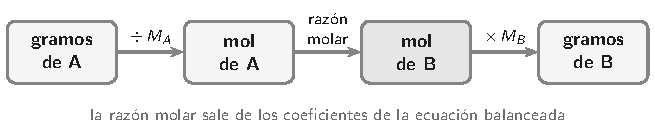
\includegraphics[max width=0.92\linewidth,max height=8.5cm]{qui/reac_camino}
\end{center}
 

\textbf{Ejemplo.} C\textsubscript{3}H\textsubscript{8} + 5 O\textsubscript{2} \ensuremath{\rightarrow} 3 CO\textsubscript{2} + 4 H\textsubscript{2}O. ¿Qué masa de CO\textsubscript{2} se forma al quemar 22 g de propano? (C = 12, H = 1, O = 16)

 

\textbf{Paso 1. Gramos a mol.} $M(\text{C}_3\text{H}_8) = 44$ g/mol: $n = \dfrac{22}{44} = 0{,}5$ mol.

 

\textbf{Paso 2. Razón molar.} 1 mol de propano da 3 mol de CO\textsubscript{2}: $0{,}5\cdot 3 = 1{,}5$ mol.

 

\textbf{Paso 3. Mol a gramos.} $m = 1{,}5\cdot 44 = 66$ g de CO\textsubscript{2}.

  
\begin{ejemplo}[{Ejemplo resuelto}] Fe + S \ensuremath{\rightarrow} FeS. ¿Qué masa máxima de FeS se forma con 112 g de Fe (56 g/mol) y exceso de S (32 g/mol)?\par \textbf{Paso 1.} $n(\text{Fe}) = \dfrac{112}{56} = 2$ mol.\par \textbf{Paso 2.} Razón 1 : 1: se forman 2 mol de FeS.\par \textbf{Paso 3.} $M(\text{FeS}) = 88$ g/mol: $2\cdot 88 = 176$ g.\par \textbf{Comprobación:} reaccionan 112 g de Fe y $2\cdot 32 = 64$ g de S: $112 + 64 = 176$ g. \ding{52}\end{ejemplo}
 
\begin{ojo}[{Error típico}] Saltarse los mol y aplicar la razón molar a los gramos: «1 : 3, entonces 22 g de propano dan 66 g de CO\textsubscript{2}» acierta aquí de casualidad, porque las dos masas molares son 44. En general falla.\end{ojo}
\subsection{Reactivo limitante y reactivo en exceso}
Para hacer un sándwich necesitas 2 panes y 1 lámina de queso. Si tienes 10 panes y 3 láminas, solo haces 3 sándwiches y sobran 4 panes: el queso \textbf{limita}.

 

En una reacción pasa lo mismo. El \textbf{reactivo limitante} es el que se acaba primero y decide cuánto producto se forma. El otro es el \textbf{reactivo en exceso}: parte de él sobra.

 
\begin{center}
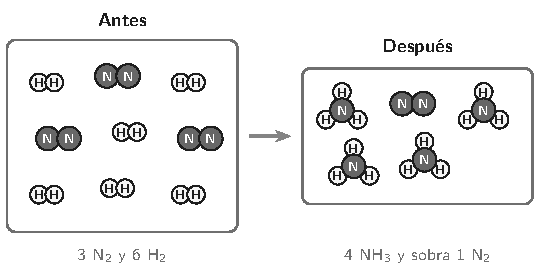
\includegraphics[max width=0.92\linewidth,max height=8.5cm]{qui/reac_limitante}
\end{center}
 

N\textsubscript{2} + 3 H\textsubscript{2} \ensuremath{\rightarrow} 2 NH\textsubscript{3}. Con 3 N\textsubscript{2} y 6 H\textsubscript{2}: los 6 H\textsubscript{2} alcanzan para 2 N\textsubscript{2}, y forman 4 NH\textsubscript{3}. Sobra 1 N\textsubscript{2}. El H\textsubscript{2} es el limitante, aunque haya más moléculas de H\textsubscript{2} que de N\textsubscript{2}.

  
\begin{clave}[{Método del cociente}] 1. Pasa cada reactivo a mol. 2. Divide los mol de cada uno por su coeficiente. 3. El \textbf{menor cociente} es el limitante. 4. Calcula el producto con el limitante.\par En el ejemplo: N\textsubscript{2}: $\dfrac{3}{1} = 3$; H\textsubscript{2}: $\dfrac{6}{3} = 2$. El menor es el del H\textsubscript{2}.\end{clave}
 
\begin{ojo}[{Error típico}] Elegir como limitante el reactivo del que hay menos mol o menos gramos. Lo que importa es cuánto hay \textbf{comparado con cuánto se necesita}: por eso se divide por el coeficiente.\end{ojo}
 
\begin{ojo}[{Otro error}] Calcular el producto con el reactivo en exceso. Da una cantidad mayor que la real, porque el limitante se acaba antes.\end{ojo}
\subsection{La tabla inicial -- reacciona -- final}
Una tabla ordena todo el cálculo y muestra cuánto sobra. Ejemplo: CH\textsubscript{4} + 2 O\textsubscript{2} \ensuremath{\rightarrow} CO\textsubscript{2} + 2 H\textsubscript{2}O, con 16 g de CH\textsubscript{4} (1 mol) y 96 g de O\textsubscript{2} (3 mol).

 

\textbf{Paso 1. Limitante.} CH\textsubscript{4}: $\dfrac{1}{1} = 1$; O\textsubscript{2}: $\dfrac{3}{2} = 1{,}5$. El limitante es el CH\textsubscript{4}.

 

\textbf{Paso 2. Tabla (en mol).} Lo que reacciona sale de la razón molar con el limitante.

 
\begin{center}\small
\begin{tabular}{@{}lllll@{}}
\toprule
 & \textbf{CH\textsubscript{4}} & \textbf{O\textsubscript{2}} & \textbf{CO\textsubscript{2}} & \textbf{H\textsubscript{2}O} \\
\midrule
Inicial & 1 & 3 & 0 & 0 \\
Reacciona / se forma & \ensuremath{-}1 & \ensuremath{-}2 & +1 & +2 \\
Final & 0 & 1 & 1 & 2 \\
\bottomrule
\end{tabular}
\end{center}
 

\textbf{Paso 3. Lee el resultado.} Se forman 1 mol de CO\textsubscript{2} (44 g) y 2 mol de H\textsubscript{2}O (36 g). Sobra 1 mol de O\textsubscript{2} (32 g).

  
\begin{clave}[{Comprobación con Lavoisier}] Masa inicial: $16 + 96 = 112$ g. Masa final: $32 + 44 + 36 = 112$ g. \ding{52} La masa de lo que sobra se cuenta en el final.\end{clave}
 
\begin{clave}[{Tablas de ensayos}] En la PAES aparecen tablas con varios ensayos: uno de los reactivos se mantiene fijo y el otro aumenta. Mientras el producto crece al aumentar un reactivo, ese reactivo es el limitante. Cuando el producto deja de crecer, el limitante pasó a ser el otro.\end{clave}
 
\begin{ojo}[{Ojo}] El reactivo limitante queda en 0 al final. Si en tu tabla un reactivo termina negativo, elegiste mal el limitante.\end{ojo}
\subsection{Lo clave del tema}
\begin{center}\small
\begin{tabularx}{\linewidth}{@{}>{\raggedright\arraybackslash\hsize=0.92\hsize}X>{\raggedright\arraybackslash\hsize=1.08\hsize}X@{}}
\toprule
\textbf{Situación} & \textbf{Qué hacer} \\
\midrule
Tengo mol, busco mol & multiplico por $\dfrac{\text{coef. de lo que busco}}{\text{coef. de lo que tengo}}$ \\
Tengo gramos, busco gramos & g \ensuremath{\rightarrow} mol (÷ $M$) \ensuremath{\rightarrow} razón molar \ensuremath{\rightarrow} mol \ensuremath{\rightarrow} g (× $M$) \\
Me dan cantidades de dos reactivos & busco el limitante: menor cociente mol / coeficiente \\
Preguntan cuánto sobra & inicial \ensuremath{-} lo que reaccionó con el limitante \\
\bottomrule
\end{tabularx}
\end{center}
 
\begin{clave}[{Recuerda}] · La razón molar es en mol: 2 H\textsubscript{2} + O\textsubscript{2} son 2 mol de H\textsubscript{2} (4 g) con 1 mol de O\textsubscript{2} (32 g).\par · En N\textsubscript{2}O\textsubscript{5} + H\textsubscript{2}O \ensuremath{\rightarrow} 2 HNO\textsubscript{3}, formar 4 mol de HNO\textsubscript{3} requiere $4\cdot\dfrac{1}{2} = 2$ mol de N\textsubscript{2}O\textsubscript{5}.\par · El limitante se elige dividiendo por los coeficientes: en N\textsubscript{2} + 3 H\textsubscript{2}, con 3 mol de N\textsubscript{2} y 6 mol de H\textsubscript{2}, $\dfrac{6}{3} = 2 < \dfrac{3}{1} = 3$: limita el H\textsubscript{2}.\par · El producto siempre se calcula con el reactivo limitante.\par · La masa de producto es solo lo que reaccionó; lo que sobra no es producto.\end{clave}
 
\begin{clave}[{Método PAES}] 1. Revisa que la ecuación esté balanceada. 2. Pasa todos los datos a mol. 3. Si hay dos reactivos, divide por los coeficientes y elige el limitante. 4. Usa la razón molar con el limitante. 5. Vuelve a gramos si te los piden. 6. Comprueba con la conservación de la masa.\end{clave}
\begin{elejemplo}{PAES Regular 2026, adaptada}
Una profesora escribe la siguiente ecuación balanceada, que representa la reacción entre aluminio y cloro para formar cloruro de aluminio:

\begin{center}
2 Al (s) + 3 Cl\textsubscript{2} (g) \ensuremath{\rightarrow} 2 AlCl\textsubscript{3} (s)
\end{center}

De acuerdo con la ecuación, ¿cuál es la máxima cantidad de AlCl\textsubscript{3} que se forma a partir de 27 g de Al y 213 g de Cl\textsubscript{2}?

Masas atómicas (g/mol): Al = 27; Cl = 35,5.
\alts{0,5 mol}{1,0 mol}{2,0 mol}{4,0 mol}
\solucion{\textbf{Paso 1. ¿Qué nos piden?} La cantidad máxima de producto. Nos dan cantidades de los dos reactivos, así que primero hay que ver cuál se acaba antes: el reactivo limitante.

\textbf{Paso 2. Pasa a mol.} Al: $n = \dfrac{27}{27} = 1$ mol. Cl\textsubscript{2}: $M = 2\cdot 35{,}5 = 71$ g/mol, así que $n = \dfrac{213}{71} = 3$ mol.

\textbf{Paso 3. Divide por los coeficientes.} Al: $\dfrac{1}{2} = 0{,}5$. Cl\textsubscript{2}: $\dfrac{3}{3} = 1$. El menor cociente es el del Al: el aluminio es el reactivo limitante.

\textbf{Paso 4. Producto con el limitante.} 2 mol de Al forman 2 mol de AlCl\textsubscript{3} (razón 1 : 1). Con 1 mol de Al se forma 1 mol de AlCl\textsubscript{3}.

\textbf{Paso 5. Tabla (en mol).}

\begin{center}\small
\begin{tabular}{@{}llll@{}}
\toprule
 & \textbf{Al} & \textbf{Cl\textsubscript{2}} & \textbf{AlCl\textsubscript{3}} \\
\midrule
Inicial & 1 & 3 & 0 \\
Reacciona / se forma & \ensuremath{-}1 & $-1\cdot\dfrac{3}{2} = -1{,}5$ & +1 \\
Final & 0 & 1,5 & 1 \\
\bottomrule
\end{tabular}
\end{center}

\textbf{Respuesta:} 1,0 mol de AlCl\textsubscript{3}.

\textbf{Comprobación:} con Lavoisier. Masa inicial: $27 + 213 = 240$ g. Masa final: AlCl\textsubscript{3}, $1\cdot(27 + 3\cdot 35{,}5) = 133{,}5$ g, más el Cl\textsubscript{2} que sobra, $1{,}5\cdot 71 = 106{,}5$ g. Total: $133{,}5 + 106{,}5 = 240$ g. \ding{52}

\textbf{¿Por qué no las otras?} 0,5 mol es el cociente del Al ($\dfrac{1}{2}$), que solo sirve para comparar; no es la cantidad de producto. 2,0 mol se calcula con el Cl\textsubscript{2}, el reactivo en exceso ($3\cdot\dfrac{2}{3} = 2$): para eso harían falta 2 mol de Al y solo hay 1. 4,0 mol suma los mol de los reactivos ($1 + 3$), y los mol no se conservan en una reacción.

\textbf{\color{cienciaD}Para recordar.} Con dos reactivos, divide sus mol por los coeficientes: el menor manda y con él se calcula el producto.}{B}
\end{elejemplo}

%% =====================================================================
%% qui_composicion
\section[Composición porcentual y fórmulas empírica y molecular]{Composición porcentual y fórmulas empírica y molecular}
\modcomun\ \ {\color{gris}\itshape Calcular el porcentaje en masa de cada elemento de un compuesto, la masa de un elemento en una muestra, y obtener la fórmula empírica y la molecular a partir de porcentajes o de masas.\par}
\subsection{Composición porcentual}
La \textbf{composición porcentual} de un compuesto dice qué porcentaje de su masa corresponde a cada elemento. Se calcula con la masa de un mol:

 
\begin{center}
$\%\,\text{elemento} = \dfrac{\text{masa del elemento en 1 mol}}{M\ \text{del compuesto}}\cdot 100$
\end{center}
 

\textbf{Ejemplo: agua, H\textsubscript{2}O} ($M = 18$ g/mol). En 1 mol hay $2\cdot 1 = 2$ g de H y 16 g de O.

 

$\%\,\text{H} = \dfrac{2}{18}\cdot 100 \approx 11{,}1\%$ y $\%\,\text{O} = \dfrac{16}{18}\cdot 100 \approx 88{,}9\%$.

 
\begin{center}\small
\begin{tabular}{@{}lll@{}}
\toprule
\textbf{Compuesto} & \textbf{$M$ (g/mol)} & \textbf{Composición} \\
\midrule
MgO & 40 & Mg $\dfrac{24}{40} = 60\%$ · O $40\%$ \\
CaCO\textsubscript{3} & 100 & Ca 40 \% · C 12 \% · O 48 \% \\
SO\textsubscript{3} & 80 & S $\dfrac{32}{80} = 40\%$ · O 60 \% \\
\bottomrule
\end{tabular}
\end{center}
  
\begin{clave}[{Siempre suman 100 \%}] Si conoces todos los porcentajes menos uno, el que falta es 100 menos la suma de los otros. Te sirve para comprobar o para hallar el oxígeno «por diferencia».\end{clave}
 
\begin{clave}[{No depende de la muestra}] Por la ley de Proust, el porcentaje es el mismo en 1 g o en 1 tonelada del compuesto puro. Una muestra de 10 g de MgO y otra de 25 g tienen ambas 60 \% de Mg; lo que cambia es la \textbf{masa} de Mg (6 g y 15 g).\end{clave}
 
\begin{ojo}[{Error típico}] Olvidar el subíndice. En H\textsubscript{2}O la masa de H en un mol es $2\cdot 1 = 2$ g, no 1 g. En CaCO\textsubscript{3} la masa de O es $3\cdot 16 = 48$ g.\end{ojo}
\subsection{Masa de un elemento en una muestra y comparar porcentajes}
\textbf{Masa de un elemento en una muestra.} Se multiplica la masa de la muestra por la fracción del elemento.

 
\begin{ejemplo}[{Ejemplo resuelto}] ¿Qué masa de oxígeno hay en 80 g de SO\textsubscript{3}? (S = 32, O = 16)\par \textbf{Paso 1.} $M(\text{SO}_3) = 32 + 48 = 80$ g/mol. En 80 g hay 48 g de O.\par \textbf{Paso 2.} La muestra pesa justo 80 g (1 mol): tiene \textbf{48 g} de O.\par Si la muestra fuera de 200 g: $200\cdot\dfrac{48}{80} = 200\cdot 0{,}6 = 120$ g de O.\end{ejemplo}
 

\textbf{Otro camino:} pasa la muestra a mol y multiplica por los átomos del elemento. 200 g de SO\textsubscript{3} son $\dfrac{200}{80} = 2{,}5$ mol; tienen $2{,}5\cdot 3 = 7{,}5$ mol de O, o sea $7{,}5\cdot 16 = 120$ g. \ding{52}

  

\textbf{Comparar porcentajes sin calculadora.} Para saber qué compuesto tiene mayor porcentaje de un elemento, mira cuánta masa de «lo demás» acompaña a cada átomo de ese elemento: mientras menos lo acompañe, mayor su porcentaje.

 
\begin{center}\small
\begin{tabular}{@{}lll@{}}
\toprule
\textbf{Óxido} & \textbf{O por cada N} & \textbf{\% de N} \\
\midrule
N\textsubscript{2}O & 0,5 & 63,6 \% \\
NO & 1 & 46,7 \% \\
N\textsubscript{2}O\textsubscript{3} & 1,5 & 36,8 \% \\
NO\textsubscript{2} & 2 & 30,4 \% \\
N\textsubscript{2}O\textsubscript{5} & 2,5 & 25,9 \% \\
\bottomrule
\end{tabular}
\end{center}
 
\begin{ojo}[{Error típico}] Creer que el compuesto con más átomos de N en la fórmula tiene más porcentaje de N. N\textsubscript{2}O\textsubscript{5} tiene 2 N, pero es el de menor porcentaje: cada N viene con 2,5 O.\end{ojo}
\subsection{Fórmula molecular, empírica y estructural}
\begin{center}
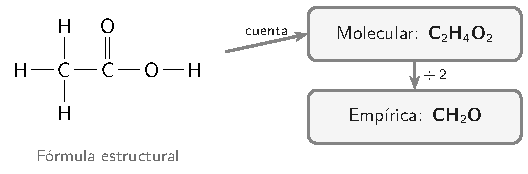
\includegraphics[max width=0.92\linewidth,max height=8.5cm]{qui/reac_formulas}
\end{center}
 
\begin{center}\small
\begin{tabularx}{\linewidth}{@{}>{\raggedright\arraybackslash\hsize=0.52\hsize}X>{\raggedright\arraybackslash\hsize=1.48\hsize}X@{}}
\toprule
\textbf{Fórmula} & \textbf{Qué muestra} \\
\midrule
Estructural & cómo están unidos los átomos \\
Molecular & cuántos átomos de cada elemento hay en \textbf{una molécula} \\
Empírica & la proporción \textbf{más simple} de números enteros entre los átomos \\
\bottomrule
\end{tabularx}
\end{center}
  
\begin{center}\small
\begin{tabular}{@{}lll@{}}
\toprule
\textbf{Sustancia} & \textbf{Molecular} & \textbf{Empírica} \\
\midrule
glucosa & C\textsubscript{6}H\textsubscript{12}O\textsubscript{6} & CH\textsubscript{2}O \\
benceno & C\textsubscript{6}H\textsubscript{6} & CH \\
agua oxigenada & H\textsubscript{2}O\textsubscript{2} & HO \\
eteno & C\textsubscript{2}H\textsubscript{4} & CH\textsubscript{2} \\
agua & H\textsubscript{2}O & H\textsubscript{2}O (ya es la más simple) \\
\bottomrule
\end{tabular}
\end{center}
 
\begin{clave}[{Cómo se obtiene la empírica}] Divide todos los subíndices de la molecular por su máximo común divisor. Si no se pueden dividir, la empírica es igual a la molecular.\end{clave}
 
\begin{ojo}[{Contar desde una estructura}] Cuenta los H de cada carbono y también los de los grupos OH, NH\textsubscript{2} o COOH. Olvidar el H del OH es el error más común. Además, varias sustancias pueden tener la misma empírica: CH\textsubscript{2}O es la de la glucosa, del ácido acético y del metanal.\end{ojo}
\subsection{Fórmula empírica a partir de porcentajes o masas}
\textbf{Los pasos:}

 

\textbf{1. Gramos.} Si te dan porcentajes, supón 100 g de compuesto: cada porcentaje pasa a ser gramos.

 

\textbf{2. Mol.} Divide los gramos de cada elemento por su masa atómica.

 

\textbf{3. Divide por el menor.} Divide todos los resultados por el más pequeño.

 

\textbf{4. Enteros.} Si sale algo como 1,5 multiplica todo por 2; si sale 1,33 o 1,67, por 3; si sale 1,25, por 4.

 
\begin{ejemplo}[{Ejemplo resuelto}] Un óxido de hierro tiene 70 \% de Fe y 30 \% de O (Fe = 56, O = 16).\par \textbf{1.} En 100 g: 70 g de Fe y 30 g de O.\par \textbf{2.} Fe: $\dfrac{70}{56} = 1{,}25$ mol. O: $\dfrac{30}{16} = 1{,}875$ mol.\par \textbf{3.} Dividimos por 1,25: Fe 1 y O 1,5.\par \textbf{4.} Multiplicamos por 2: Fe 2 y O 3. Fórmula empírica: \textbf{Fe\textsubscript{2}O\textsubscript{3}}.\end{ejemplo}
  
\begin{clave}[{Desde masas}] Si te dan masas de cada elemento, salta el paso 1. Ejemplo: un compuesto tiene 14 g de N y 24 g de O. N: $\dfrac{14}{14} = 1$ mol. O: $\dfrac{24}{16} = 1{,}5$ mol. Razón 1 : 1,5 = 2 : 3: \textbf{N\textsubscript{2}O\textsubscript{3}}.\end{clave}
 
\begin{ojo}[{Error típico}] Usar los porcentajes o las masas como subíndices, sin dividir por la masa atómica: 70 \% Fe y 30 \% O \textbf{no} es Fe\textsubscript{7}O\textsubscript{3}. Los subíndices cuentan átomos (mol), no gramos.\end{ojo}
 
\begin{ojo}[{Otro error}] Redondear 1,5 a 1 o a 2. Solo se redondea lo que está muy cerca de un entero (1,98 \ensuremath{\rightarrow} 2); 1,5 obliga a multiplicar.\end{ojo}
\subsection{De la fórmula empírica a la molecular}
La fórmula molecular es la empírica multiplicada por un número entero $n$. Para hallar $n$ se necesita la masa molar del compuesto:

 
\begin{center}
$n = \dfrac{M\ \text{del compuesto}}{M\ \text{de la fórmula empírica}}$
\end{center}
 
\begin{ejemplo}[{Ejemplo resuelto}] Un compuesto tiene 40 \% de C, 6,7 \% de H y 53,3 \% de O, y su masa molar es 180 g/mol.\par \textbf{1.} En 100 g: C $\dfrac{40}{12}\approx 3{,}33$ mol; H $\dfrac{6{,}7}{1} = 6{,}7$ mol; O $\dfrac{53{,}3}{16}\approx 3{,}33$ mol.\par \textbf{2.} Dividimos por 3,33: C 1, H 2, O 1. Empírica: CH\textsubscript{2}O, con $M = 12 + 2 + 16 = 30$ g/mol.\par \textbf{3.} $n = \dfrac{180}{30} = 6$. Molecular: C\textsubscript{6}H\textsubscript{12}O\textsubscript{6} (glucosa).\end{ejemplo}
  
\begin{clave}[{¿Cómo se miden esos porcentajes?}] En el laboratorio se quema una masa conocida del compuesto y se masan el CO\textsubscript{2} y el H\textsubscript{2}O que se forman. De ahí se calculan las masas de C y de H de la muestra; el O se obtiene por diferencia. Con esas masas se calcula la fórmula empírica. En la PAES este procedimiento puede aparecer como pregunta de habilidades.\end{clave}
 
\begin{ojo}[{Error típico}] Multiplicar solo un elemento por $n$. Se multiplican \textbf{todos} los subíndices: (CH\textsubscript{2}O)\textsubscript{6} = C\textsubscript{6}H\textsubscript{12}O\textsubscript{6}.\end{ojo}
 
\begin{clave}[{Control}] La masa molar de la fórmula molecular debe dar exactamente la del enunciado: $6\cdot 12 + 12\cdot 1 + 6\cdot 16 = 180$. \ding{52}\end{clave}
\subsection{Lo clave del tema}
\begin{center}\small
\begin{tabularx}{\linewidth}{@{}>{\raggedright\arraybackslash\hsize=0.93\hsize}X>{\raggedright\arraybackslash\hsize=1.07\hsize}X@{}}
\toprule
\textbf{Me piden} & \textbf{Hago} \\
\midrule
\% de un elemento & $\dfrac{\text{subíndice}\cdot\text{masa atómica}}{M}\cdot 100$ \\
masa de un elemento en una muestra & masa de la muestra $\cdot\ \dfrac{\text{masa del elemento en 1 mol}}{M}$ \\
fórmula empírica desde \% o masas & gramos \ensuremath{\rightarrow} mol (÷ masa atómica) \ensuremath{\rightarrow} ÷ el menor \ensuremath{\rightarrow} enteros \\
fórmula molecular & $n = \dfrac{M}{M_{\text{empírica}}}$ y multiplico todos los subíndices \\
fórmula empírica desde la molecular & divido los subíndices por su máximo común divisor \\
\bottomrule
\end{tabularx}
\end{center}
 
\begin{clave}[{Recuerda}] · Los porcentajes se pasan a moles: C $\dfrac{80}{12}$, H $\dfrac{20}{1}$, razón 1 : 3, fórmula CH\textsubscript{3}.\par · \% H en H\textsubscript{2}O $= \dfrac{2}{18}\approx 11{,}1\%$: cuenta el subíndice.\par · Una razón 1 : 1,5 se multiplica por 2: Fe\textsubscript{2}O\textsubscript{3}.\par · El ácido butanoico es C\textsubscript{4}H\textsubscript{8}O\textsubscript{2} (incluye el H del OH).\par · La composición porcentual no depende de la muestra: cambia la masa de Mg, no su \%.\end{clave}
 
\begin{clave}[{Método PAES}] 1. Calcula la masa molar con cuidado. 2. Para porcentajes, divide la masa del elemento en un mol por $M$; para comparar, mira cuánto acompaña a cada átomo del elemento. 3. Para fórmulas, trabaja siempre en mol: divide por la masa atómica, luego por el menor, y lleva a enteros. 4. Comprueba: los porcentajes suman 100 y la masa molar de tu fórmula coincide con la del enunciado.\end{clave}
\begin{elejemplo}{PAES Invierno 2026, adaptada}
En una actividad sobre la composición de los óxidos de nitrógeno, una profesora presenta la siguiente información sobre cuatro compuestos formados solo por nitrógeno y oxígeno:

¿Cuál de los compuestos tiene la fórmula empírica N\textsubscript{2}O\textsubscript{3}?

Masas atómicas (g/mol): N = 14; O = 16.
\begin{center}\small
\begin{tabular}{@{}lll@{}}
\toprule
\textbf{Compuesto} & \textbf{Masa de N (g)} & \textbf{Masa de O (g)} \\
\midrule
\textbf{1} & 7 & 8 \\
\textbf{2} & 14 & 24 \\
\textbf{3} & 28 & 16 \\
\textbf{4} & 14 & 40 \\
\bottomrule
\end{tabular}
\end{center}
\alts{El compuesto 1.}{El compuesto 2.}{El compuesto 3.}{El compuesto 4.}
\solucion{\textbf{Paso 1. ¿Qué nos piden?} El compuesto cuya proporción de átomos es N : O = 2 : 3. Las masas no se comparan directamente: hay que pasarlas a mol, porque los subíndices cuentan átomos.

\textbf{Paso 2. Qué buscamos.} En N\textsubscript{2}O\textsubscript{3} hay 1,5 átomos de O por cada átomo de N. Buscamos el compuesto con razón $\dfrac{n_{\text{O}}}{n_{\text{N}}} = 1{,}5$.

\textbf{Paso 3. Compuesto 1.} N: $\dfrac{7}{14} = 0{,}5$ mol. O: $\dfrac{8}{16} = 0{,}5$ mol. Razón 1 : 1, fórmula empírica NO.

\textbf{Paso 4. Compuesto 2.} N: $\dfrac{14}{14} = 1$ mol. O: $\dfrac{24}{16} = 1{,}5$ mol. Razón 1 : 1,5; multiplicando por 2, 2 : 3. Fórmula empírica \textbf{N\textsubscript{2}O\textsubscript{3}}.

\textbf{Paso 5. Revisa los otros.} Compuesto 3: N $\dfrac{28}{14} = 2$, O $\dfrac{16}{16} = 1$: N\textsubscript{2}O. Compuesto 4: N 1, O $\dfrac{40}{16} = 2{,}5$: razón 2 : 5, N\textsubscript{2}O\textsubscript{5}.

\textbf{Respuesta:} el compuesto 2.

\textbf{Comprobación:} en N\textsubscript{2}O\textsubscript{3} hay $2\cdot 14 = 28$ g de N por cada $3\cdot 16 = 48$ g de O. Razón en masa $28 : 48 = 14 : 24$, justo la del compuesto 2. \ding{52}

\textbf{¿Por qué no las otras?} El compuesto 1 tiene masas parecidas (7 y 8), lo que puede hacer pensar en «casi 1 : 1 en masa», pero en mol es NO. El compuesto 3 tiene el doble de N que de O en mol: es N\textsubscript{2}O; quien lo elige compara los gramos (28 y 16) sin dividir por la masa atómica. El compuesto 4 es N\textsubscript{2}O\textsubscript{5}: tiene 2,5 O por cada N, más de lo necesario.

\textbf{\color{cienciaD}Para recordar.} Para la fórmula empírica, divide cada masa por su masa atómica y compara los mol, nunca los gramos.}{B}
\end{elejemplo}

\chapter{Soluciones químicas}
%% =====================================================================
%% qui_soluciones
\section[Características de las soluciones y solubilidad]{Características de las soluciones y solubilidad}
\modcomun\ \ {\color{gris}\itshape Soluto y solvente, propiedades de las soluciones, soluciones insaturadas, saturadas y sobresaturadas, solubilidad y los factores que la cambian, y cómo leer una curva de solubilidad.\par}
\subsection{¿Qué es una solución?}
Una \textbf{solución} (o disolución) es una \textbf{mezcla homogénea}: a simple vista, e incluso con microscopio, se ve una sola fase. Tiene dos tipos de componentes:

 
\begin{itemize}
  \item \textbf{Soluto}: lo que se disuelve. Por lo general está en menor cantidad, y puede haber más de uno.
  \item \textbf{Solvente} (o disolvente): lo que disuelve. Está en mayor cantidad y define el estado de la solución. El agua es el solvente más común, por eso se le llama \textbf{solvente universal}; las soluciones en agua se llaman \textbf{acuosas}.
\end{itemize}
 

Las masas se suman: \textbf{masa de solución = masa de soluto + masa de solvente}. Si disuelves 10 g de sal en 90 g de agua, obtienes 100 g de solución. Los volúmenes, en cambio, no siempre se suman exactamente (50 mL de etanol con 50 mL de agua dan unos 97 mL). Por eso los problemas dicen "considere volúmenes aditivos" cuando quieren que los sumes.

 
\begin{center}
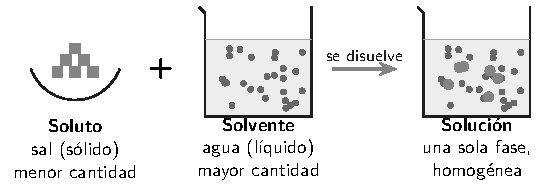
\includegraphics[max width=0.92\linewidth,max height=8.5cm]{qui/sol_particulas}
\end{center}
  
\begin{clave}[{Soluciones en los tres estados}] \begin{center}\small
\begin{tabularx}{\linewidth}{@{}>{\raggedright\arraybackslash\hsize=0.48\hsize}X>{\raggedright\arraybackslash\hsize=0.78\hsize}X>{\raggedright\arraybackslash\hsize=1.74\hsize}X@{}}
\toprule
\textbf{Solución} & \textbf{Soluto en solvente} & \textbf{Ejemplo} \\
\midrule
Gaseosa & gas en gas & aire (O\textsubscript{2}, Ar y CO\textsubscript{2} en N\textsubscript{2}) \\
Líquida & sólido en líquido & agua de mar, suero fisiológico \\
Líquida & gas en líquido & bebida gaseosa (CO\textsubscript{2} en agua) \\
Líquida & líquido en líquido & vinagre (ácido acético en agua), vino \\
Sólida & sólido en sólido & bronce (estaño en cobre), acero (carbono en hierro) \\
\bottomrule
\end{tabularx}
\end{center}\end{clave}
 
\begin{ojo}[{¿Quién es el solvente?}] El que define el estado de la solución y, casi siempre, el que está en mayor cantidad. En el aire es el nitrógeno (78 \%). En una bebida con mucha azúcar, el solvente sigue siendo el agua.\end{ojo}
\subsection{Propiedades de las soluciones}
Una solución verdadera cumple con todo esto:

 
\begin{itemize}
  \item \textbf{Una sola fase}: es homogénea; cualquier gota tiene la misma composición.
  \item \textbf{Es transparente}, aunque puede tener color (el sulfato de cobre(II) en agua es azul).
  \item \textbf{El soluto no sedimenta}: aunque la dejes reposar días, no se va al fondo.
  \item \textbf{No se separa por filtración}: el soluto atraviesa el papel filtro. Sí se separa con métodos que cambian de estado, como la \textbf{evaporación} (queda el sólido) o la \textbf{destilación}.
  \item \textbf{Composición variable}: puedes poner más o menos soluto (hasta un límite) y sigue siendo solución. Un compuesto, en cambio, tiene composición fija.
  \item \textbf{Conduce la corriente} solo si el soluto es un \textbf{electrolito} (sales como NaCl, ácidos, bases), que libera iones. Si el soluto es molecular, como el azúcar o el etanol, no conduce.
\end{itemize}
  
\begin{ejemplo}[{Ejemplo: agua con sal y agua con arena}] \begin{center}\small
\begin{tabularx}{\linewidth}{@{}>{\raggedright\arraybackslash\hsize=0.88\hsize}X>{\raggedright\arraybackslash\hsize=0.80\hsize}X>{\raggedright\arraybackslash\hsize=1.32\hsize}X@{}}
\toprule
\textbf{Propiedad} & \textbf{Agua con sal} & \textbf{Agua con arena} \\
\midrule
Fases & 1 & 2 \\
¿Sedimenta al reposar? & No & Sí \\
¿Se separa al filtrar? & No & Sí \\
¿Conduce la corriente? & Sí (iones Na\textsuperscript{+} y Cl\textsuperscript{\ensuremath{-}}) & No (como el agua pura, casi nada) \\
Tipo de mezcla & Solución & Mezcla heterogénea \\
\bottomrule
\end{tabularx}
\end{center}\end{ejemplo}
 
\begin{ojo}[{Disolver no es reaccionar}] Cuando el azúcar se disuelve, sus moléculas se separan y se rodean de agua, pero siguen siendo azúcar: es un cambio físico. Si evaporas el agua, recuperas el azúcar.\end{ojo}
\subsection{Insaturada, saturada y sobresaturada}
\textbf{1. Diluida o concentrada.} Es una comparación entre soluciones: un jugo con poco polvo está \textbf{diluido} y uno con mucho, \textbf{concentrado}. Son términos relativos: no dicen si cabe más soluto.

 

\textbf{2. Según la solubilidad.} Cada soluto tiene un máximo que se disuelve en cierta cantidad de solvente a una temperatura: su \textbf{solubilidad}. Comparando con ese máximo:

 
\begin{itemize}
  \item \textbf{Insaturada}: tiene menos soluto que el máximo. Si agregas más, se disuelve.
  \item \textbf{Saturada}: tiene justo el máximo. Si agregas más, queda sin disolver en el fondo, y la solución sigue saturada.
  \item \textbf{Sobresaturada}: tiene disuelto más que el máximo. Se logra disolviendo en caliente y enfriando sin mover el recipiente. Es \textbf{inestable}: un golpe o un cristal "semilla" hace que el exceso precipite de golpe, y queda saturada.
\end{itemize}
 
\begin{center}
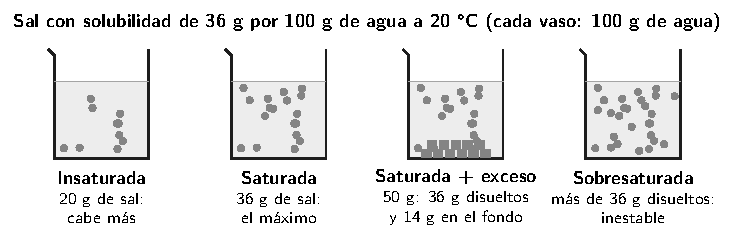
\includegraphics[max width=0.92\linewidth,max height=8.5cm]{qui/sol_clasificacion}
\end{center}
  
\begin{ejemplo}[{Ejemplo resuelto}] La solubilidad de una sal es 36 g por 100 g de agua a 20 °C. ¿Qué pasa si agregas 50 g de sal a 200 g de agua a 20 °C?\par \textbf{Paso 1.} Escala el máximo a la masa de agua: 200 g de agua disuelven $2\cdot 36 = 72$ g.\par \textbf{Paso 2.} Compara: $50 < 72$, así que se disuelve todo. La solución es \textbf{insaturada} y todavía caben $72 - 50 = 22$ g.\par \textbf{Paso 3.} ¿Y si los 50 g van en solo 100 g de agua? Se disuelven 36 g y quedan $50 - 36 = 14$ g en el fondo: \textbf{saturada} con exceso.\end{ejemplo}
 
\begin{ojo}[{Sobresaturada no es "con sal en el fondo"}] Si queda sólido en el fondo, la solución está \textbf{saturada}. Sobresaturada es tener disuelto más que el máximo, sin sólido, y es inestable.\end{ojo}
\subsection{La solubilidad y sus factores}
La \textbf{solubilidad} es la máxima cantidad de soluto que se disuelve en una cantidad dada de solvente a cierta temperatura (y presión). Se suele dar en \textbf{g de soluto por 100 g de agua}. Depende de tres factores:

 

\textbf{1. Naturaleza del soluto y del solvente.} "Lo semejante disuelve a lo semejante": las sustancias \textbf{polares} o iónicas se disuelven en solventes polares, como el agua; las \textbf{apolares}, en solventes apolares. La sal y el azúcar se disuelven en agua; el aceite no, y forma dos fases. El yodo (apolar) casi no se disuelve en agua, pero sí en hexano.

 

\textbf{2. Temperatura.} En la mayoría de los sólidos, la solubilidad \textbf{aumenta} al subir la temperatura (algunas sales, como el carbonato de litio, hacen lo contrario). En los \textbf{gases} siempre \textbf{disminuye}: el agua tibia retiene menos gas. Por eso una bebida tibia pierde el gas más rápido y un río con agua tibia tiene menos oxígeno para los peces.

 

\textbf{3. Presión.} Afecta casi solo a los \textbf{gases}: a mayor presión del gas sobre el líquido, más gas se disuelve (ley de Henry). La bebida se embotella con CO\textsubscript{2} a alta presión; al abrirla, la presión baja y el gas escapa en burbujas.

  
\begin{center}
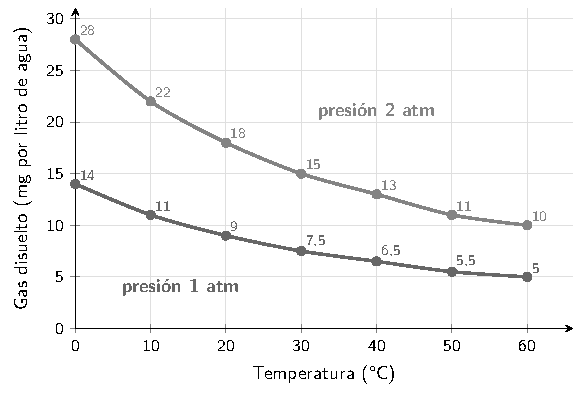
\includegraphics[max width=0.92\linewidth,max height=8.5cm]{qui/sol_gas}
\end{center}
 

Datos inventados para un gas cualquiera, con la forma real: al calentar baja la solubilidad, y al duplicar la presión se duplica.

 
\begin{ojo}[{Solubilidad no es rapidez}] Agitar o moler el soluto hace que se disuelva \textbf{más rápido}, pero no cambia \textbf{cuánto} se disuelve como máximo. De los factores de la vida diaria, solo la temperatura (y, en gases, la presión) cambia la solubilidad.\end{ojo}
 
\begin{clave}[{Pistas en un ensayo de solubilidad}] Dos líquidos que se mezclan en una sola fase son del mismo tipo (los dos polares o los dos apolares). Si forman dos fases, son de distinto tipo; arriba queda el menos denso.\end{clave}
\subsection{Curvas de solubilidad}
\begin{center}
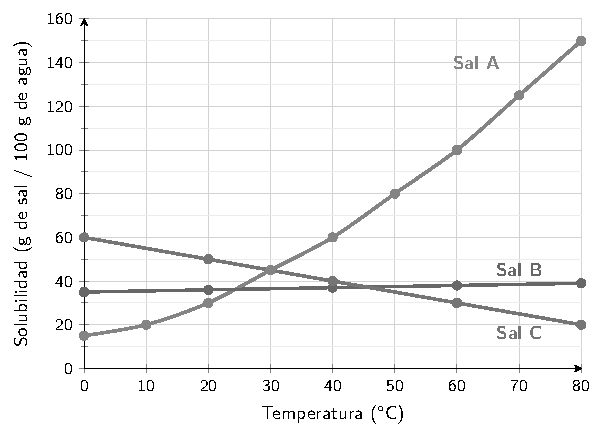
\includegraphics[max width=0.92\linewidth,max height=8.5cm]{qui/sol_curvas}
\end{center}
 

Una \textbf{curva de solubilidad} muestra la solubilidad de una sustancia (eje vertical) a cada temperatura (eje horizontal). El gráfico tiene datos inventados para tres sales: la A se comporta como el nitrato de potasio (sube mucho al calentar), la B como el cloruro de sodio (casi no cambia) y la C como el carbonato de litio (baja al calentar).

 

\textbf{Cómo leerla.} Sube desde la temperatura hasta la curva y lee a la izquierda: la sal A a 40 °C tiene una solubilidad de 60 g por 100 g de agua.

 

\textbf{Dónde está tu solución.} Ubica el punto (temperatura; g de soluto por 100 g de agua): \textbf{justo en la curva}, saturada; \textbf{debajo}, insaturada; \textbf{por encima}, sobresaturada (o saturada con el exceso sin disolver). Si dos curvas se cortan, las dos sales tienen la misma solubilidad a esa temperatura: A y C, a 30 °C, con 45 g.

  
\begin{ejemplo}[{Ejemplo resuelto: masa que cristaliza al enfriar}] Una solución saturada de sal A con 200 g de agua a 60 °C se enfría hasta 20 °C. ¿Cuántos gramos de sal cristalizan?\par \textbf{Paso 1. Lee la curva.} A 60 °C: 100 g por 100 g de agua. A 20 °C: 30 g por 100 g de agua.\par \textbf{Paso 2. Escala a 200 g de agua} (multiplica por 2): a 60 °C hay 200 g de sal disuelta; a 20 °C caben solo 60 g.\par \textbf{Paso 3. Lo que no cabe, cristaliza:} $200 - 60 = 140$ g.\par \textbf{Comprobación:} 60 g disueltos + 140 g de cristales = 200 g, toda la sal que había. \ding{52}\end{ejemplo}
 
\begin{ojo}[{Escala por la masa de agua}] La curva está hecha para 100 g de agua. Con 50 g de agua, divide por 2; con 300 g, multiplica por 3. Y con una sal como la C pasa al revés: cristaliza al \textbf{calentar}.\end{ojo}
\subsection{Lo clave del tema}
\begin{center}\small
\begin{tabularx}{\linewidth}{@{}>{\raggedright\arraybackslash\hsize=0.96\hsize}X>{\raggedright\arraybackslash\hsize=1.04\hsize}X@{}}
\toprule
\textbf{Concepto} & \textbf{Lo esencial} \\
\midrule
Solución & Mezcla homogénea de soluto y solvente. masa solución = masa soluto + masa solvente. \\
Propiedades & Una fase, no sedimenta, no se separa al filtrar, composición variable; conduce si el soluto es electrolito. \\
Insaturada / saturada / sobresaturada & Menos / igual / más soluto disuelto que la solubilidad. \\
Solubilidad & Máximo de soluto por 100 g de agua a una temperatura. \\
Factores & Naturaleza (semejante disuelve a semejante); temperatura (sólidos: casi siempre sube; gases: baja); presión (solo gases: sube). \\
Curva & En la curva, saturada; debajo, insaturada. Cristaliza = lo disuelto antes \ensuremath{-} lo que cabe después, escalado a la masa de agua. \\
\bottomrule
\end{tabularx}
\end{center}
  
\begin{clave}[{Recuerda}] · Si queda sal en el fondo, la solución está saturada; la sobresaturada no deja sólido.\par · La curva de solubilidad es por 100 g de agua: multiplica por (g de agua)/100.\par · Agitar solo hace que se disuelva más rápido; no cambia la solubilidad.\par · Los gases se disuelven menos al calentar y más al subir la presión.\end{clave}
 
\begin{clave}[{Método para la PAES}] 1. Identifica soluto, solvente y temperatura. 2. Si te dan la solubilidad, escálala a la masa de agua y compara. 3. En curvas, lee los dos puntos, escala y resta. 4. En experimentos, busca qué variable cambia entre ensayos y cuáles se mantienen.\end{clave}
\begin{elejemplo}{PAES Invierno 2027, adaptada}
Daniela investiga la solubilidad del cloruro de potasio (KCl) en agua a 20 °C. En tres matraces Erlenmeyer pone 100 g de agua y agrega distintas masas de KCl sólido. Agita cada mezcla durante 10 minutos, las deja reposar y registra lo que observa en la tabla. Finalmente, filtra la mezcla del matraz 3, evapora el agua del líquido filtrado y obtiene 34,0 g de KCl.\par De acuerdo con estos resultados, ¿cuál es una inferencia correcta?
\begin{center}\small
\begin{tabular}{@{}lll@{}}
\toprule
\textbf{Matraz} & \textbf{Masa de KCl agregada (g)} & \textbf{¿Queda sólido sin disolver?} \\
\midrule
\textbf{1} & 30,0 & No \\
\textbf{2} & 34,0 & No \\
\textbf{3} & 38,0 & Sí \\
\bottomrule
\end{tabular}
\end{center}
\altslargas{La solución del matraz 1 está saturada.}{La solución del matraz 2 contiene la máxima masa de KCl que se disuelve en 100 g de agua a 20 °C.}{La solución del matraz 3 contiene 38,0 g de KCl disueltos.}{La solución del matraz 3 está sobresaturada, porque se agregó más KCl que su solubilidad.}
\solucion{\textbf{Paso 1. ¿Qué nos piden?} Una inferencia: una conclusión que se deduce de los datos. Primero hay que encontrar la solubilidad del KCl a 20 °C.

 

\textbf{Paso 2. Encuentra la solubilidad.} En el matraz 3 quedó sólido sin disolver, así que el líquido de arriba es una solución \textbf{saturada}. Al filtrar se separa el sólido; al evaporar el agua del líquido filtrado queda justo lo que estaba disuelto: 34,0 g. Entonces la solubilidad es \textbf{34 g de KCl por 100 g de agua} a 20 °C.

 

\textbf{Paso 3. Clasifica cada matraz} (todos tienen 100 g de agua):

 
\begin{itemize}
  \item Matraz 1: $30 < 34$, se disuelve todo y caben 4 g más: \textbf{insaturada}.
  \item Matraz 2: $34 = 34$, se disuelve todo y no cabe nada más: \textbf{saturada}, con la máxima masa posible.
  \item Matraz 3: se disuelven 34 g y quedan $38 - 34 = 4$ g en el fondo: \textbf{saturada con exceso}.
\end{itemize}
 

\textbf{Respuesta:} la solución del matraz 2 contiene la máxima masa de KCl que se disuelve en 100 g de agua a 20 °C.

 

\textbf{Comprobación:} en el matraz 3, 34 g disueltos + 4 g en el fondo = 38 g, lo que se agregó. Si Daniela secara el sólido retenido en el filtro, debería pesar unos 4 g.

 

\textbf{¿Por qué no las otras?} «Matraz 1 saturada»: tiene 30 g y el máximo es 34 g, así que aún caben 4 g. «Matraz 3 con 38,0 g disueltos»: 4 g no se disolvieron y quedaron en el filtro, por eso al evaporar se obtuvieron 34 g y no 38 g. «Matraz 3 sobresaturada»: una solución con sólido en el fondo está saturada; la sobresaturada tiene disuelto más que el máximo, sin sólido, y es inestable.

\textbf{\color{cienciaD}Para recordar.} Al filtrar una mezcla saturada y evaporar el líquido obtienes justo la solubilidad: lo que sobra quedó en el fondo, no en la solución.}{B}
\end{elejemplo}

%% =====================================================================
%% qui_conc_fisicas
\section[Concentración: \% m/m, \% m/v, \% v/v y ppm]{Concentración: \% m/m, \% m/v, \% v/v y ppm}
\modcomun\ \ {\color{gris}\itshape Qué es la concentración y cómo calcularla con las unidades físicas: porcentaje masa/masa, masa/volumen y volumen/volumen, partes por millón, y la densidad para pasar de volumen a masa.\par}
\subsection{¿Qué es la concentración?}
La \textbf{concentración} dice cuánto soluto hay en cierta cantidad de solución. No importa el tamaño del vaso, sino la \textbf{proporción}: una cucharada de un suero al 0,9 \% también está al 0,9 \%. Por eso la concentración no cambia si tomas una muestra más grande o más chica de la misma solución.

 

Las \textbf{unidades físicas} usan solo masas y volúmenes (sin moles):

 
\begin{center}\small
\begin{tabular}{@{}lll@{}}
\toprule
\textbf{Unidad} & \textbf{Significa} & \textbf{Fórmula} \\
\midrule
\% m/m & g de soluto en 100 g de solución & $\dfrac{\text{g soluto}}{\text{g solución}}\cdot 100$ \\
\% m/v & g de soluto en 100 mL de solución & $\dfrac{\text{g soluto}}{\text{mL solución}}\cdot 100$ \\
\% v/v & mL de soluto en 100 mL de solución & $\dfrac{\text{mL soluto}}{\text{mL solución}}\cdot 100$ \\
ppm & mg de soluto en 1 L (o 1 kg) de solución & $\dfrac{\text{mg soluto}}{\text{L solución}}$ \\
\bottomrule
\end{tabular}
\end{center}
  
\begin{center}
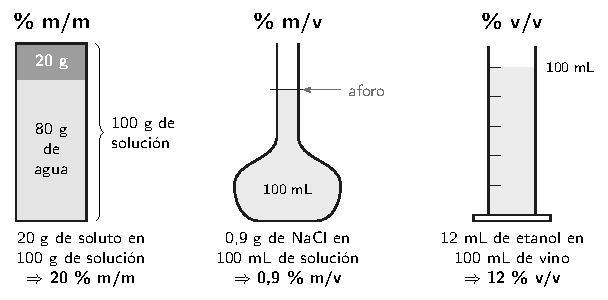
\includegraphics[max width=0.92\linewidth,max height=8.5cm]{qui/sol_porcentajes}
\end{center}
 
\begin{ojo}[{Siempre sobre la solución}] En las cuatro unidades el denominador es la \textbf{solución completa} (soluto + solvente), no el solvente solo.\end{ojo}
\subsection{Porcentaje masa/masa (\% m/m)}
Indica cuántos gramos de soluto hay en 100 g de solución:

 \[ \%\,\text{m/m} = \dfrac{m_{\text{soluto}}}{m_{\text{soluto}} + m_{\text{solvente}}}\cdot 100 \] 

\textbf{Ejemplo 1.} Se disuelven 25 g de sal en 100 g de agua. ¿Cuál es el \% m/m?

 

\textbf{Paso 1.} Masa de solución: $25 + 100 = 125$ g.

 

\textbf{Paso 2.} $\dfrac{25}{125}\cdot 100 = 20$ \%. La solución es 20 \% m/m.

 

\textbf{Ejemplo 2 (al revés).} ¿Cómo preparas 250 g de solución de azúcar al 8 \% m/m?

 

\textbf{Paso 1.} Soluto: $\dfrac{8}{100}\cdot 250 = 20$ g de azúcar.

 

\textbf{Paso 2.} Agua: lo que falta para 250 g, $250 - 20 = 230$ g.

 

\textbf{Comprobación:} $\dfrac{20}{20 + 230}\cdot 100 = \dfrac{20}{250}\cdot 100 = 8$ \%. \ding{52}

  
\begin{clave}[{Léelo como receta}] 20 \% m/m significa: 20 g de soluto por cada 100 g de solución, o sea, 20 g de soluto + 80 g de agua.\end{clave}
 
\begin{ojo}[{Error típico}] En el ejemplo 1, dividir por el agua da $\dfrac{25}{100}\cdot 100 = 25$ \%, que está mal: los 100 g son solo el solvente. La solución pesa 125 g.\end{ojo}
 
\begin{clave}[{}] La escala \textbf{Brix} de la industria del vino y los jugos es un \% m/m de azúcar: 1 °Bx es 1 g de azúcar en 100 g de solución.\end{clave}
\subsection{Porcentaje masa/volumen (\% m/v)}
Indica cuántos gramos de soluto hay en 100 mL de solución:

 \[ \%\,\text{m/v} = \dfrac{m_{\text{soluto}}\ (\text{g})}{V_{\text{solución}}\ (\text{mL})}\cdot 100 \] 

\textbf{Ejemplo 1.} El suero fisiológico es NaCl al 0,9 \% m/v. ¿Cuánto NaCl tiene una bolsa de 500 mL?

 

\textbf{Paso 1.} 0,9 g en cada 100 mL. 500 mL son 5 veces 100 mL.

 

\textbf{Paso 2.} $5 \cdot 0{,}9 = 4{,}5$ g de NaCl.

 

\textbf{Ejemplo 2.} Se disuelven 12 g de glucosa en agua hasta completar 300 mL de solución. ¿Cuál es el \% m/v?

 

\textbf{Paso 1.} $\dfrac{12}{300}\cdot 100 = 4$ \%. La solución es 4 \% m/v.

  
\begin{ojo}[{"Hasta completar" no es "se agregan"}] "Se disuelve en agua hasta completar 300 mL" significa que la \textbf{solución} mide 300 mL. "Se agregan 300 mL de agua" deja una solución de algo más de 300 mL. En \% m/v siempre va el volumen de la solución.\end{ojo}
 
\gatotip[\gatolila]{\textbf{Truco útil.} 4 \% m/v = 4 g en 100 mL = \textbf{40 g en 1 L}. Multiplicar el \% m/v por 10 te da los gramos por litro, y con eso pasas fácil a mol/L.}
\subsection{Porcentaje volumen/volumen (\% v/v)}
Se usa cuando el soluto es un líquido, como el alcohol en las bebidas. Indica cuántos mL de soluto hay en 100 mL de solución:

 \[ \%\,\text{v/v} = \dfrac{V_{\text{soluto}}\ (\text{mL})}{V_{\text{solución}}\ (\text{mL})}\cdot 100 \] 

\textbf{Ejemplo 1.} Un vino tiene 12 \% v/v de etanol (los "12 grados" de la etiqueta). ¿Cuánto etanol hay en una botella de 750 mL?

 

\textbf{Paso 1.} $\dfrac{12}{100}\cdot 750 = 90$ mL de etanol.

 

\textbf{Ejemplo 2.} Se mezclan 30 mL de etanol con agua hasta completar 200 mL. ¿Cuál es el \% v/v?

 

\textbf{Paso 1.} $\dfrac{30}{200}\cdot 100 = 15$ \%. La solución es 15 \% v/v.

  
\begin{ojo}[{Volúmenes que no se suman}] Al mezclar etanol y agua, el volumen final es un poco menor que la suma. Por eso las recetas dicen "completar hasta" un volumen. Si un problema dice "considere volúmenes aditivos", entonces sí puedes restar: en el vino, $750 - 90 = 660$ mL de agua.\end{ojo}
 
\begin{ejemplo}[{Ejemplo diario}] El alcohol gel al 70 \% v/v tiene 70 mL de etanol en cada 100 mL de gel.\end{ejemplo}
\subsection{Partes por millón (ppm)}
Para concentraciones muy bajas, como contaminantes o el flúor del agua potable, los porcentajes dan números incómodos. Se usan las \textbf{partes por millón}: 1 ppm es 1 g de soluto en 1.000.000 g de solución, o sea, \textbf{1 mg por kg}. En soluciones acuosas diluidas, 1 L pesa casi 1 kg, así que:

 \[ \text{ppm} = \dfrac{\text{mg de soluto}}{\text{L de solución}} \qquad \text{(o mg de soluto por kg, en sólidos)} \] 

\textbf{Ejemplo 1.} Un análisis encuentra 3 mg de ion fluoruro en 2 L de agua potable. $\dfrac{3\ \text{mg}}{2\ \text{L}} = 1{,}5$ ppm.

 

\textbf{Ejemplo 2.} La norma de agua potable permite hasta 0,01 mg/L de arsénico, es decir, 0,01 ppm. En 5 L de esa agua puede haber como máximo $0{,}01 \cdot 5 = 0{,}05$ mg.

  
\begin{clave}[{Para comparar}] 1 \% m/m = 1 g en 100 g = 10.000 mg en 1 kg = \textbf{10.000 ppm}.\end{clave}
 
\begin{ojo}[{Cuida las unidades}] ppm es mg por \textbf{litro} (no por mL) y por \textbf{miligramo} (no gramo). Si te dan mL, pásalos a L: 500 mL = 0,5 L. Si te dan gramos, pásalos a mg: 0,02 g = 20 mg.\end{ojo}
\subsection{La densidad: de volumen a masa}
Muchas veces te dan el volumen de una solución pero la concentración en \% m/m. La \textbf{densidad} conecta las dos cosas:

 \[ d = \dfrac{m}{V} \qquad\Rightarrow\qquad m = d\cdot V \] 

\textbf{Ejemplo.} Un frasco tiene 200 mL de solución de NaOH al 10 \% m/m, con densidad 1,2 g/mL. ¿Cuánto NaOH contiene y cuál es su \% m/v?

 

\textbf{Paso 1. Masa de la solución.} $m = 1{,}2 \cdot 200 = 240$ g.

 

\textbf{Paso 2. Masa de soluto.} El 10 \% de 240 g: $0{,}10 \cdot 240 = 24$ g de NaOH.

 

\textbf{Paso 3. \% m/v.} $\dfrac{24}{200}\cdot 100 = 12$ \% m/v.

 

\textbf{Comprobación:} \% m/v = \% m/m · densidad: $10 \cdot 1{,}2 = 12$. \ding{52}

  
\begin{ojo}[{¿Densidad de qué?}] Usa la densidad de la \textbf{solución}, no la del agua. El ácido clorhídrico comercial al 37 \% m/m tiene densidad cercana a 1,19 g/mL: 100 mL de él pesan unos 119 g, no 100 g.\end{ojo}
 
\begin{clave}[{Si d = 1 g/mL}] Los gramos y los mililitros de solución son el mismo número: 500 mL de solución pesan 500 g. Muchos problemas PAES lo dan así para simplificar.\end{clave}
\subsection{Lo clave del tema}
\begin{center}\small
\begin{tabularx}{\linewidth}{@{}>{\raggedright\arraybackslash\hsize=0.49\hsize}X>{\raggedright\arraybackslash\hsize=1.28\hsize}X>{\raggedright\arraybackslash\hsize=1.24\hsize}X@{}}
\toprule
\textbf{Unidad} & \textbf{Cálculo} & \textbf{Ejemplo} \\
\midrule
\% m/m & g soluto / g solución · 100 & 25 g en 100 g de agua \ensuremath{\rightarrow} 20 \% \\
\% m/v & g soluto / mL solución · 100 & 4,5 g en 500 mL \ensuremath{\rightarrow} 0,9 \% \\
\% v/v & mL soluto / mL solución · 100 & 90 mL en 750 mL \ensuremath{\rightarrow} 12 \% \\
ppm & mg soluto / L solución & 3 mg en 2 L \ensuremath{\rightarrow} 1,5 ppm \\
Densidad & m = d · V & 200 mL · 1,2 g/mL = 240 g \\
\bottomrule
\end{tabularx}
\end{center}
  
\begin{clave}[{Recuerda}] · \% m/m: divide por la masa de solución (soluto + agua).\par · 15 \% m/m son 15 g por cada 100 g de solución; escala a la masa real.\par · ppm = mg por L.\par · Si d \ensuremath{\neq} 1, pasa de mL a gramos con m = d · V.\end{clave}
 
\begin{clave}[{Método para la PAES}] 1. Anota qué es soluto y qué es solución, con unidades. 2. Elige la fórmula según la unidad pedida. 3. Pasa las unidades (mL \ensuremath{\leftrightarrow} L, g \ensuremath{\leftrightarrow} mg, volumen \ensuremath{\leftrightarrow} masa con la densidad). 4. Comprueba al revés: con tu resultado, ¿vuelves al dato?\end{clave}
\begin{elejemplo}{PAES Invierno 2027, adaptada}
Para preparar 0,5 L de una solución acuosa al 15 \% m/m de un compuesto soluble en agua (densidad de la solución = 1,0 g/mL), se deben mezclar
\alts{15 g del compuesto y 485 g de agua.}{75 g del compuesto y 500 g de agua.}{75 g del compuesto y 425 g de agua.}{15 g del compuesto y 85 g de agua.}
\solucion{\textbf{Paso 1. ¿Qué nos piden?} Las masas de compuesto (soluto) y de agua (solvente) que forman 0,5 L de solución al 15 \% m/m.

 

\textbf{Paso 2. Pasa el volumen a masa.} 0,5 L = 500 mL. Con la densidad: $m = d\cdot V = 1{,}0 \cdot 500 = 500$ g de solución.

 

\textbf{Paso 3. Masa de soluto.} 15 \% m/m es 15 g por cada 100 g de solución: $\dfrac{15}{100}\cdot 500 = 75$ g de compuesto.

 

\textbf{Paso 4. Masa de agua.} Lo que falta para completar 500 g: $500 - 75 = 425$ g de agua.

 

\textbf{Respuesta:} 75 g del compuesto y 425 g de agua.

 

\textbf{Comprobación:} $\dfrac{75}{75 + 425}\cdot 100 = \dfrac{75}{500}\cdot 100 = 15$ \%. \ding{52} Y la masa total, 500 g, con d = 1,0 g/mL ocupa 500 mL = 0,5 L. \ding{52}

 

\textbf{¿Por qué no las otras?} «15 g y 485 g» toma el 15 \% como 15 g totales: da $\dfrac{15}{500}\cdot 100 = 3$ \%. «75 g y 500 g» suma el soluto a 500 g de agua: la solución pesa 575 g y queda en $\dfrac{75}{575}\cdot 100 \approx 13$ \%. «15 g y 85 g» sí está al 15 \%, pero son solo 100 g de solución, no los 500 g pedidos.

\textbf{\color{cienciaD}Para recordar.} En \% m/m, masa de soluto = \% · masa de solución / 100, y el agua es lo que falta para completar la solución.}{C}
\end{elejemplo}

%% =====================================================================
%% qui_conc_quimicas
\section[Concentración molar, molal y fracción molar]{Concentración molar, molal y fracción molar}
\modcomun\ \ {\color{gris}\itshape Cómo pasar de gramos a moles y calcular la concentración molar (mol/L), la concentración molal (mol/kg de solvente) y la fracción molar; cómo se prepara una solución y cómo pasar de \% m/v a mol/L.\par}
\subsection{Del gramo al mol}
Las unidades químicas cuentan el soluto en \textbf{moles}, porque las reacciones ocurren partícula a partícula. Para pasar de gramos a moles se usa la \textbf{masa molar} ($M$, en g/mol):

 \[ n = \dfrac{m}{M} \] 

\textbf{Ejemplo 1.} Masa molar del NaOH (Na = 23, O = 16, H = 1): $23 + 16 + 1 = 40$ g/mol. Entonces 20 g de NaOH son $n = \dfrac{20}{40} = 0{,}5$ mol.

 

\textbf{Ejemplo 2.} Glucosa, C\textsubscript{6}H\textsubscript{12}O\textsubscript{6} (C = 12, H = 1, O = 16): $6\cdot 12 + 12\cdot 1 + 6\cdot 16 = 72 + 12 + 96 = 180$ g/mol. Entonces 9 g son $\dfrac{9}{180} = 0{,}05$ mol.

 

\textbf{Al revés:} $m = n \cdot M$. Por ejemplo, 0,1 mol de NaOH pesan $0{,}1 \cdot 40 = 4$ g.

  
\begin{ojo}[{Divide, no multipliques}] De gramos a moles se divide por la masa molar. Si multiplicas, $20 \cdot 40 = 800$, el número no tiene sentido: 20 g de algo no pueden ser 800 mol.\end{ojo}
 
\begin{clave}[{Masas molares que conviene tener a mano}] (la PAES las entrega)\par H\textsubscript{2}O = 18 g/mol · NaOH = 40 g/mol · NaCl = 58,5 g/mol · KOH = 56 g/mol · HCl = 36,5 g/mol · C\textsubscript{6}H\textsubscript{12}O\textsubscript{6} = 180 g/mol · C\textsubscript{2}H\textsubscript{5}OH = 46 g/mol\end{clave}
\subsection{Concentración molar (mol/L)}
La \textbf{concentración molar} (antes llamada molaridad) indica cuántos moles de soluto hay en \textbf{1 litro de solución}:

 \[ C = \dfrac{n_{\text{soluto}}\ (\text{mol})}{V_{\text{solución}}\ (\text{L})} \] 

\textbf{Ejemplo 1.} Se disuelven 20 g de NaOH ($M$ = 40 g/mol) en agua hasta completar 500 mL. Moles: $\dfrac{20}{40} = 0{,}5$ mol. Volumen: 500 mL = 0,5 L. $C = \dfrac{0{,}5}{0{,}5} = 1$ mol/L.

 

\textbf{Ejemplo 2 (al revés).} ¿Cuántos gramos de glucosa ($M$ = 180 g/mol) se necesitan para 250 mL de solución 0,2 mol/L? Moles: $n = C\cdot V = 0{,}2 \cdot 0{,}25 = 0{,}05$ mol. Masa: $0{,}05 \cdot 180 = 9$ g.

 
\begin{clave}[{Así se prepara}] 1. Masa el soluto. 2. Disuélvelo en un poco de agua dentro de un \textbf{matraz aforado}. 3. Agrega agua hasta la marca (el aforo). 4. Tapa y agita. Así el volumen final de solución es exacto.\end{clave}
  
\begin{center}
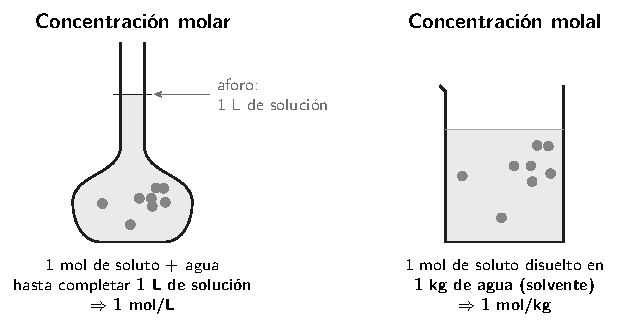
\includegraphics[max width=0.92\linewidth,max height=8.5cm]{qui/sol_molar_molal}
\end{center}
 
\begin{ojo}[{Dos errores clásicos}] 1. Dejar el volumen en mL: $\dfrac{0{,}5}{500} = 0{,}001$ está mal; pasa 500 mL a 0,5 L. 2. Disolver el soluto en 250 mL de agua: la solución queda con más de 250 mL. Se completa \textbf{hasta} 250 mL.\end{ojo}
\subsection{Concentración molal (mol/kg)}
La \textbf{concentración molal} (molalidad) indica cuántos moles de soluto hay por cada \textbf{kilogramo de solvente} (no de solución):

 \[ b = \dfrac{n_{\text{soluto}}\ (\text{mol})}{m_{\text{solvente}}\ (\text{kg})} \] 

\textbf{Ejemplo 1.} Se disuelven 20 g de NaOH ($M$ = 40 g/mol) en 500 g de agua. Moles: 0,5 mol. Solvente: 500 g = 0,5 kg. $b = \dfrac{0{,}5}{0{,}5} = 1$ mol/kg.

 

\textbf{Ejemplo 2.} 9 g de glucosa ($M$ = 180 g/mol) en 250 g de agua: $\dfrac{0{,}05}{0{,}25} = 0{,}2$ mol/kg.

  
\begin{center}\small
\begin{tabularx}{\linewidth}{@{}>{\raggedright\arraybackslash\hsize=1.09\hsize}X>{\raggedright\arraybackslash\hsize=1.01\hsize}X>{\raggedright\arraybackslash\hsize=0.89\hsize}X@{}}
\toprule
 & \textbf{Molar} & \textbf{Molal} \\
\midrule
Unidad & mol/L & mol/kg \\
Denominador & L de \textbf{solución} & kg de \textbf{solvente} \\
Se mide con & matraz aforado & balanza \\
¿Cambia con la temperatura? & Sí (el volumen se dilata) & No (la masa no cambia) \\
\bottomrule
\end{tabularx}
\end{center}
 
\begin{ojo}[{Ojo}] En molal el denominador es \textbf{solo el solvente} y va en \textbf{kilogramos}: 500 g de agua son 0,5 kg. Si divides por gramos, el resultado sale 1.000 veces más chico.\end{ojo}
\subsection{Fracción molar}
La \textbf{fracción molar} ($X$) de un componente es la parte de los moles totales que le corresponde:

 \[ X_{\text{soluto}} = \dfrac{n_{\text{soluto}}}{n_{\text{soluto}} + n_{\text{solvente}}} \] 

No tiene unidades, está entre 0 y 1, y las fracciones de todos los componentes \textbf{suman 1}.

 

\textbf{Ejemplo.} Se mezclan 46 g de etanol ($M$ = 46 g/mol) con 72 g de agua ($M$ = 18 g/mol).

 

\textbf{Paso 1. Moles.} Etanol: $\dfrac{46}{46} = 1$ mol. Agua: $\dfrac{72}{18} = 4$ mol. Total: 5 mol.

 

\textbf{Paso 2. Fracciones.} $X_{\text{etanol}} = \dfrac{1}{5} = 0{,}2$ y $X_{\text{agua}} = \dfrac{4}{5} = 0{,}8$.

 

\textbf{Comprobación:} $0{,}2 + 0{,}8 = 1$. \ding{52}

  
\begin{ojo}[{Tres errores frecuentes}] · Dividir por los moles del solvente: $\dfrac{1}{4} = 0{,}25$. El denominador es el \textbf{total}.\par · Usar masas en vez de moles: $\dfrac{46}{118} \approx 0{,}39$ es una fracción de masa, no molar.\par · Entregar la fracción del otro componente (0,8 en vez de 0,2).\end{ojo}
 
\begin{clave}[{Para qué sirve}] Se usa en mezclas de líquidos y de gases (el aire tiene $X_{\text{N}_2} \approx 0{,}78$) y en las propiedades que dependen del número de partículas.\end{clave}
\subsection{Pasar de una unidad a otra}
\textbf{De \% m/v a mol/L.} Multiplica el \% m/v por 10 para tener gramos por litro y divide por la masa molar.

 

\textbf{Ejemplo.} NaOH al 4 \% m/v ($M$ = 40 g/mol): 4 g en 100 mL = 40 g en 1 L. $\dfrac{40}{40} = 1$ mol en 1 L, o sea, \textbf{1 mol/L}.

 

\textbf{De mol/L a \% m/v.} NaCl 2 mol/L ($M$ = 58,5 g/mol): en 1 L hay $2\cdot 58{,}5 = 117$ g, o sea, 11,7 g en 100 mL: \textbf{11,7 \% m/v}.

 

\textbf{De \% m/m a mol/L, con densidad.} NaOH al 10 \% m/m con d = 1,2 g/mL. Toma 1 L de solución.

 

\textbf{Paso 1.} Masa de 1 L: $1{,}2 \cdot 1.000 = 1.200$ g.

 

\textbf{Paso 2.} Soluto: el 10 \% de 1.200 g = 120 g de NaOH.

 

\textbf{Paso 3.} Moles: $\dfrac{120}{40} = 3$ mol en 1 L: \textbf{3 mol/L}.

  
\begin{clave}[{Fórmula atajo}] $C\ (\text{mol/L}) = \dfrac{\%\,\text{m/v} \cdot 10}{M}$\end{clave}
 
\begin{ojo}[{Elige 1 L de base}] Cuando la concentración no depende de cuánto tengas, imagina 1 L (o 100 g) de solución: los cálculos salen con números redondos.\end{ojo}
\subsection{Lo clave del tema}
\begin{center}\small
\begin{tabularx}{\linewidth}{@{}>{\raggedright\arraybackslash\hsize=0.53\hsize}X>{\raggedright\arraybackslash\hsize=1.14\hsize}X>{\raggedright\arraybackslash\hsize=1.33\hsize}X@{}}
\toprule
\textbf{Unidad} & \textbf{Fórmula} & \textbf{Ejemplo} \\
\midrule
Moles & $n = m / M$ & 20 g de NaOH = 0,5 mol \\
Molar & mol de soluto / L de solución & 0,5 mol en 500 mL \ensuremath{\rightarrow} 1 mol/L \\
Molal & mol de soluto / kg de solvente & 0,5 mol en 500 g de agua \ensuremath{\rightarrow} 1 mol/kg \\
Fracción molar & $n_i$ / $n_{\text{total}}$, sin unidades & 1 mol etanol + 4 mol agua \ensuremath{\rightarrow} 0,2 \\
\% m/v \ensuremath{\rightarrow} mol/L & \% m/v · 10 / M & 4 \% de NaOH \ensuremath{\rightarrow} 1 mol/L \\
\bottomrule
\end{tabularx}
\end{center}
  
\begin{clave}[{Recuerda}] · Molaridad: primero pasa los gramos a moles ($m/M$).\par · Volumen en litros (molar) y masa de solvente en kg (molal).\par · Molalidad: divide solo por la masa del solvente.\par · Para preparar V mL de solución, completa hasta V mL en un matraz aforado.\end{clave}
 
\begin{clave}[{Método para la PAES}] 1. Pasa la masa a moles. 2. Mira el denominador que pide la unidad (L de solución, kg de solvente o moles totales). 3. Convierte unidades. 4. Comprueba al revés: $n = C\cdot V$ debe devolverte los moles.\end{clave}
\begin{elejemplo}{PAES Invierno 2027, adaptada}
En una clase de química, la profesora pide preparar 250 mL de una solución acuosa de hidróxido de sodio (NaOH) de concentración 0,4 mol/L (masa molar del NaOH = 40 g/mol). ¿Cuál de los siguientes procedimientos es el adecuado?
\altslargas{Masar 4 g de NaOH y disolverlos en 250 mL de agua.}{Masar 4 g de NaOH, disolverlos en un poco de agua dentro de un matraz aforado de 250 mL y luego agregar agua hasta el aforo.}{Masar 16 g de NaOH, disolverlos en un poco de agua dentro de un matraz aforado de 250 mL y luego agregar agua hasta el aforo.}{Masar 4 g de NaOH, disolverlos en agua y completar con agua hasta 1 L de solución.}
\solucion{\textbf{Paso 1. ¿Qué nos piden?} Dos cosas: la masa correcta de NaOH y la forma correcta de lograr 250 mL \textbf{de solución}.

 

\textbf{Paso 2. Moles necesarios.} $n = C\cdot V = 0{,}4\ \text{mol/L} \cdot 0{,}25\ \text{L} = 0{,}1$ mol.

 

\textbf{Paso 3. Masa.} $m = n\cdot M = 0{,}1 \cdot 40 = 4$ g de NaOH.

 

\textbf{Paso 4. Procedimiento.} El volumen de la fórmula es el de la \textbf{solución}. Por eso se disuelven los 4 g en un poco de agua dentro de un matraz aforado de 250 mL y se completa con agua hasta la marca: el volumen final es exactamente 250 mL.

 

\textbf{Respuesta:} masar 4 g de NaOH, disolverlos en un poco de agua dentro de un matraz aforado de 250 mL y agregar agua hasta el aforo.

 

\textbf{Comprobación:} $C = \dfrac{4/40}{0{,}25} = \dfrac{0{,}1}{0{,}25} = 0{,}4$ mol/L. \ding{52}

 

\textbf{¿Por qué no las otras?} «4 g en 250 mL de agua»: la masa está bien, pero el soluto agrega volumen y la solución queda con más de 250 mL, así que la concentración queda bajo 0,4 mol/L. «16 g hasta el aforo»: 16 g son 0,4 mol; en 0,25 L dan $\dfrac{0{,}4}{0{,}25} = 1{,}6$ mol/L (confunde 0,4 mol/L con 0,4 mol). «4 g hasta 1 L»: da $\dfrac{0{,}1}{1} = 0{,}1$ mol/L.

\textbf{\color{cienciaD}Para recordar.} Para preparar una solución: n = C · V, m = n · M, y se completa HASTA el volumen pedido en un matraz aforado.}{B}
\end{elejemplo}

%% =====================================================================
%% qui_dilucion
\section[Dilución y mezclas de soluciones]{Dilución y mezclas de soluciones}
\modcomun\ \ {\color{gris}\itshape Qué pasa al agregar agua a una solución, cómo usar C\textsubscript{1}·V\textsubscript{1} = C\textsubscript{2}·V\textsubscript{2} para calcular volúmenes y concentraciones, cuánta agua agregar, diluciones sucesivas y la concentración al mezclar soluciones del mismo soluto.\par}
\subsection{¿Qué es diluir?}
\textbf{Diluir} es agregar solvente a una solución. Pasan tres cosas:

 
\begin{itemize}
  \item Los \textbf{moles (y gramos) de soluto no cambian}: no agregaste soluto ni lo sacaste.
  \item El \textbf{volumen aumenta}.
  \item La \textbf{concentración baja}: el mismo soluto queda repartido en más volumen.
\end{itemize}
 

El \textbf{factor de dilución} dice cuántas veces creció el volumen: $\dfrac{V_2}{V_1}$. La concentración baja esas mismas veces. Si llevas 5 mL de una solución a 25 mL en un matraz aforado, el volumen crece 5 veces y la concentración queda en \textbf{un quinto} de la original, sea cual sea la unidad (\% m/m, mol/L\dots{}).

 

Lo contrario, \textbf{evaporar solvente}, sube la concentración: los moles siguen iguales en menos volumen.

  
\begin{center}
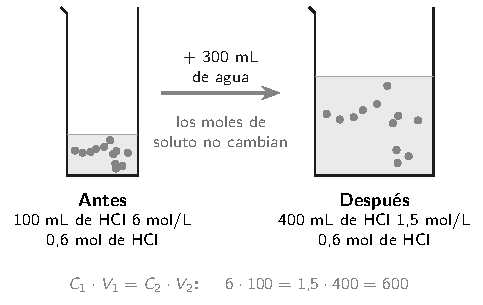
\includegraphics[max width=0.92\linewidth,max height=8.5cm]{qui/sol_dilucion}
\end{center}
 
\begin{ojo}[{Diluir no saca soluto}] "Al diluir hay menos soluto" es falso. Hay el mismo soluto; lo que hay es menos soluto \textbf{por cada mL}.\end{ojo}
\subsection{La fórmula C\textsubscript{1}·V\textsubscript{1} = C\textsubscript{2}·V\textsubscript{2}}
Como los moles no cambian, $n_1 = n_2$. Y como $n = C\cdot V$:

 \[ C_1 \cdot V_1 = C_2 \cdot V_2 \] 

El subíndice 1 es la solución inicial (concentrada) y el 2, la final (diluida). Con tres datos, despejas el cuarto.

 

\textbf{Ejemplo.} Tienes 100 mL de HCl 6 mol/L y quieres llevarlo a 1,5 mol/L. ¿Qué volumen final tendrá y cuánta agua agregas?

 

\textbf{Paso 1.} $6 \cdot 100 = 1{,}5 \cdot V_2$.

 

\textbf{Paso 2.} $V_2 = \dfrac{600}{1{,}5} = 400$ mL.

 

\textbf{Paso 3. Agua:} $V_2 - V_1 = 400 - 100 = 300$ mL.

 

\textbf{Comprobación:} moles antes, $6 \cdot 0{,}1 = 0{,}6$ mol; después, $1{,}5 \cdot 0{,}4 = 0{,}6$ mol. \ding{52}

  
\begin{clave}[{Unidades}] Los dos volúmenes deben ir en la misma unidad (los dos en mL o los dos en L), y las dos concentraciones también. No hace falta pasar a litros si ambos están en mL.\end{clave}
 
\begin{ojo}[{V\textsubscript{2} es el volumen final, no el agua}] El error más común es responder 400 mL cuando preguntan cuánta agua agregar. Agua = $V_2 - V_1$ (con volúmenes aditivos).\end{ojo}
\subsection{Cuánta agua agregar}
\textbf{Ejemplo 1.} Se tienen 0,5 L de H\textsubscript{2}SO\textsubscript{4} 4,0 mol/L y se necesita 0,2 mol/L. ¿Cuánta agua se agrega (volúmenes aditivos)?

 

\textbf{Paso 1.} $V_2 = \dfrac{C_1 V_1}{C_2} = \dfrac{4{,}0 \cdot 0{,}5}{0{,}2} = 10$ L.

 

\textbf{Paso 2.} Agua: $10 - 0{,}5 = 9{,}5$ L.

 

\textbf{Ejemplo 2, con \% m/v.} Se tienen 50 mL de NaOH al 4 \% m/v ($M$ = 40 g/mol) y se quiere 0,5 mol/L.

 

\textbf{Paso 1. Pasa a mol/L.} 4 \% m/v = 40 g/L = 1 mol/L.

 

\textbf{Paso 2.} $V_2 = \dfrac{1 \cdot 50}{0{,}5} = 100$ mL. Agua: $100 - 50 = 50$ mL.

  
\begin{clave}[{Preparar desde una solución madre}] Quieres 1 L de NaOH 0,03 mol/L a partir de NaOH 1,0 mol/L. $V_1 = \dfrac{0{,}03 \cdot 1.000}{1{,}0} = 30$ mL de solución madre, más agua hasta 1.000 mL: \textbf{30 mL + 970 mL de agua}. Mezclar 30 mL con 1.000 mL de agua daría 1.030 mL y una concentración un poco menor.\end{clave}
 
\begin{ojo}[{Las dos concentraciones en la misma unidad}] Si una está en \% m/v y la otra en mol/L, convierte primero.\end{ojo}
\subsection{Diluciones sucesivas y material}
A veces se diluye en dos pasos. Se resuelve un paso a la vez: la concentración final del primero es la inicial del segundo.

 

\textbf{Ejemplo.} A 500 mL de NaCl 1,5 mol/L se le agrega 1 L de agua (solución X). Luego se toman 10 mL de X y se completan con agua hasta 50 mL (solución Y). ¿Concentración de Y?

 

\textbf{Paso 1. Solución X.} Volumen: $500 + 1.000 = 1.500$ mL. $C_X = \dfrac{1{,}5 \cdot 500}{1.500} = 0{,}5$ mol/L.

 

\textbf{Paso 2. Solución Y.} $C_Y = \dfrac{0{,}5 \cdot 10}{50} = 0{,}1$ mol/L.

 

\textbf{Comprobación con factores:} el primer paso diluye 3 veces y el segundo 5 veces: en total 15 veces. $\dfrac{1{,}5}{15} = 0{,}1$. \ding{52}

  
\begin{clave}[{Material de laboratorio}] · \textbf{Pipeta} (aforada o graduada): para tomar un volumen exacto de la solución concentrada.\par · \textbf{Matraz aforado}: para completar un volumen final exacto. Es el material indispensable cuando la variable que se controla es el volumen final.\par · Vaso de precipitados y probeta: medidas aproximadas; no sirven para un volumen final exacto.\end{clave}
 
\begin{ojo}[{"Toma 10 mL de X"}] Tomar una parte de una solución no cambia su concentración: los 10 mL de X siguen siendo 0,5 mol/L.\end{ojo}
\subsection{Mezclas de soluciones del mismo soluto}
Al mezclar dos soluciones del \textbf{mismo soluto}, los moles se suman y los volúmenes también (si son aditivos):

 \[ C_f = \dfrac{C_1 V_1 + C_2 V_2}{V_1 + V_2} \] 
\begin{center}
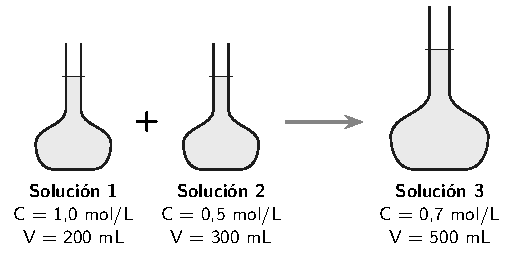
\includegraphics[max width=0.92\linewidth,max height=8.5cm]{qui/sol_mezcla_0}
\end{center}
 

\textbf{Ejemplo.} 200 mL de NaCl 1,0 mol/L + 300 mL de NaCl 0,5 mol/L.

 

\textbf{Paso 1. Moles.} $1{,}0 \cdot 0{,}2 = 0{,}2$ mol y $0{,}5 \cdot 0{,}3 = 0{,}15$ mol. Total: 0,35 mol.

 

\textbf{Paso 2. Volumen.} $0{,}2 + 0{,}3 = 0{,}5$ L.

 

\textbf{Paso 3.} $C_f = \dfrac{0{,}35}{0{,}5} = 0{,}7$ mol/L.

  
\begin{clave}[{Para comprobar}] La concentración final siempre queda \textbf{entre} las dos iniciales (0,5 < 0,7 < 1,0), más cerca de la que aporta más volumen. Si mezclas soluciones de \textbf{igual} concentración, la mezcla tiene esa misma concentración, aunque tenga el doble de soluto.\end{clave}
 
\begin{clave}[{Con tres soluciones}] 10 mL de HCl 1,0 mol/L + 20 mL de HCl 0,5 mol/L + 50 mL de HCl 0,2 mol/L: moles $0{,}01 + 0{,}01 + 0{,}01 = 0{,}03$ mol en 0,08 L: $\dfrac{0{,}03}{0{,}08} = 0{,}375$ mol/L.\end{clave}
 
\begin{ojo}[{No promedies las concentraciones}] $\dfrac{1{,}0 + 0{,}5}{2} = 0{,}75$ está mal, salvo que los volúmenes sean iguales. Suma moles y divide por el volumen total.\end{ojo}
\subsection{Lo clave del tema}
\begin{center}\small
\begin{tabularx}{\linewidth}{@{}>{\raggedright\arraybackslash\hsize=0.73\hsize}X>{\raggedright\arraybackslash\hsize=1.27\hsize}X@{}}
\toprule
\textbf{Situación} & \textbf{Qué hacer} \\
\midrule
Dilución & $C_1 V_1 = C_2 V_2$; los moles no cambian. \\
Agua a agregar & $V_2 - V_1$ (volúmenes aditivos). \\
Factor de dilución & $V_2 / V_1$: la concentración se divide por ese número. \\
Dos diluciones seguidas & Una a la vez, o multiplica los factores. \\
Mezcla del mismo soluto & $C_f = (C_1V_1 + C_2V_2)/(V_1 + V_2)$; queda entre las dos. \\
Evaporar solvente & Sube la concentración; los moles no cambian. \\
\bottomrule
\end{tabularx}
\end{center}
  
\begin{clave}[{Recuerda}] · El agua agregada es $V_2 - V_1$.\par · Al diluir, el volumen final es mayor que el inicial.\par · Al mezclar soluciones, suma moles y suma volúmenes.\par · Al diluir, los moles de soluto no cambian; solo baja la concentración.\end{clave}
 
\begin{clave}[{Método para la PAES}] 1. Escribe qué es 1 (inicial) y qué es 2 (final). 2. Iguala moles. 3. Fíjate si piden volumen final o agua agregada. 4. Comprueba: la concentración diluida debe ser menor y la de una mezcla, intermedia.\end{clave}
\begin{elejemplo}{PAES Invierno 2026, adaptada}
Algunos productos para el alisado del cabello contienen hidróxido de sodio (NaOH, masa molar = 40 g/mol), cuya concentración no debe superar cierto valor para evitar daños. Considerando volúmenes aditivos, ¿qué volumen de agua se debe agregar a 100 mL de una solución de NaOH al 2 \% m/v para obtener una solución de concentración 0,2 mol/L?
\alts{40 mL}{150 mL}{250 mL}{900 mL}
\solucion{\textbf{Paso 1. ¿Qué nos piden?} El volumen de \textbf{agua} que hay que agregar, no el volumen final. Las dos concentraciones vienen en unidades distintas, así que primero hay que igualarlas.

 

\textbf{Paso 2. Pasa el 2 \% m/v a mol/L.} 2 \% m/v son 2 g en 100 mL, o sea, 20 g en 1 L. En moles: $\dfrac{20}{40} = 0{,}5$ mol en 1 L. Entonces $C_1 = 0{,}5$ mol/L.

 

\textbf{Paso 3. Usa la dilución.} $C_1 V_1 = C_2 V_2$: $0{,}5 \cdot 100 = 0{,}2 \cdot V_2$, así que $V_2 = \dfrac{50}{0{,}2} = 250$ mL.

 

\textbf{Paso 4. Agua a agregar.} $250 - 100 = 150$ mL.

 

\textbf{Respuesta:} 150 mL.

 

\textbf{Comprobación:} moles de NaOH: al inicio, $0{,}5 \cdot 0{,}1 = 0{,}05$ mol (son los 2 g: $2/40 = 0{,}05$); al final, $0{,}2 \cdot 0{,}25 = 0{,}05$ mol. \ding{52}

 

\textbf{¿Por qué no las otras?} 250 mL es el volumen final, no el agua agregada. 40 mL despeja la fórmula al revés: $\dfrac{0{,}2 \cdot 100}{0{,}5}$, un volumen final menor que el inicial, lo que es imposible al diluir. 900 mL toma el 2 \% como si fuera 2 mol/L: $V_2 = \dfrac{2 \cdot 100}{0{,}2} = 1.000$ mL y resta 100 mL.

\textbf{\color{cienciaD}Para recordar.} Antes de usar C\textsubscript{1}V\textsubscript{1} = C\textsubscript{2}V\textsubscript{2}, pon las dos concentraciones en la misma unidad; y si piden agua, resta V\textsubscript{1}.}{B}
\end{elejemplo}

\chapter{Habilidades científicas}
%% =====================================================================
%% qui_hab_investigacion
\section[Investigar: preguntas, hipótesis y variables]{Investigar: preguntas, hipótesis y variables}
\modcomun\ \ {\color{gris}\itshape Cómo se arma una investigación en química: pregunta investigable, hipótesis y predicción, variables independiente, dependiente y controladas, grupo control, procedimiento e instrumentos, y la diferencia entre ley, teoría y modelo.\par}
\subsection{La investigación científica paso a paso}
Entre un cuarto y un tercio de las preguntas de la PAES de Ciencias no miden cuánta química sabes, sino si sabes \textbf{pensar como investigador}: reconocer la pregunta, la hipótesis, las variables y la conclusión de un experimento. Todas siguen el mismo esquema:

 
\begin{center}
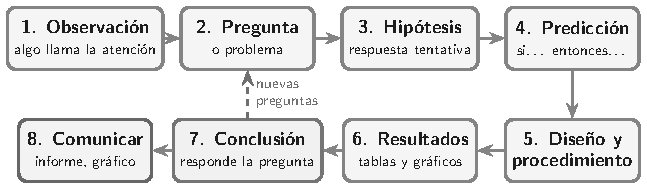
\includegraphics[max width=0.92\linewidth,max height=8.5cm]{qui/hab_ciclo}
\end{center}
  

\textbf{Un ejemplo completo.}

 

\textbf{1. Observación.} Una estudiante nota que una tableta efervescente burbujea más rápido en agua tibia que en agua fría.

 

\textbf{2. Pregunta.} ¿Cómo influye la temperatura del agua en el tiempo que tarda la tableta en disolverse?

 

\textbf{3. Hipótesis.} A mayor temperatura del agua, menor es el tiempo de disolución.

 

\textbf{4. Predicción.} Si la hipótesis es correcta, la tableta se disolverá antes en agua a 40 °C que en agua a 10 °C.

 

\textbf{5. Procedimiento.} Pone tabletas iguales en 200 mL de agua a 10, 25 y 40 °C y mide con cronómetro el tiempo hasta que dejan de burbujear.

 

\textbf{6. Resultados.} 64 s, 40 s y 22 s.

 

\textbf{7. Conclusión.} En el rango estudiado, a mayor temperatura del agua, menor fue el tiempo de disolución: los datos apoyan la hipótesis.

  
\begin{clave}[{Pregunta investigable}] Es una pregunta que se puede responder \textbf{midiendo} algo. Casi siempre relaciona dos variables: «¿cómo influye A en B?».\end{clave}
 
\begin{clave}[{¿Investigable o no?}] · «¿Influye la concentración de HCl en la rapidez con que reacciona el magnesio?»: sí, se mide.\par · «¿Es el cobre el metal más bonito?»: no, es una opinión.\par · «¿Qué pasará con la química dentro de mil años?»: no, no se puede medir hoy.\end{clave}
 
\begin{ojo}[{Ojo}] La pregunta de investigación tiene que calzar con los datos. Si en la tabla solo cambia el tipo de fruta y se mide la vitamina C, la pregunta es «¿cómo varía la vitamina C en distintas frutas?», no «¿qué factores determinan la vitamina C?».\end{ojo}
\subsection{Hipótesis y predicción}
La \textbf{hipótesis} es una explicación o respuesta tentativa a la pregunta. Tiene tres rasgos:

 
\begin{itemize}
  \item Se escribe \textbf{antes} del experimento.
  \item Relaciona la variable que se cambia con la que se mide: «la concentración influye en la rapidez», «a mayor temperatura, mayor solubilidad».
  \item Se puede poner a prueba, y podría resultar falsa.
\end{itemize}
 

La \textbf{predicción} es más concreta: dice qué resultado se espera en \textbf{este} experimento si la hipótesis es cierta. Suele tener la forma «si\dots{}, entonces\dots{}».

 
\begin{center}\small
\begin{tabularx}{\linewidth}{@{}>{\raggedright\arraybackslash\hsize=1.00\hsize}X>{\raggedright\arraybackslash\hsize=1.00\hsize}X@{}}
\toprule
\textbf{Hipótesis} & \textbf{Predicción} \\
\midrule
La concentración de HCl influye en la rapidez de su reacción con magnesio. & Con HCl 2,0 mol/L el globo se inflará más en 1 minuto que con HCl 0,5 mol/L. \\
A menor tamaño de las partículas, más rápida es la disolución. & El azúcar flor se disolverá antes que el azúcar en terrones. \\
\bottomrule
\end{tabularx}
\end{center}
  
\begin{ejemplo}[{Ejemplo resuelto: ¿qué hipótesis se puso a prueba?}] Unos estudiantes preparan 100 mL de cuatro soluciones de KMnO\textsubscript{4} de 1,0; 0,2; 0,01 y 0,002 mol/L. Todas a 25 °C, agitadas 60 s, en frascos iguales y con la misma luz. Después observan la tonalidad.\par \textbf{Paso 1.} ¿Qué cambia de un frasco a otro? Solo la concentración.\par \textbf{Paso 2.} ¿Qué se observa? La tonalidad del color.\par \textbf{Paso 3.} La hipótesis une las dos: «la concentración de una solución influye en la tonalidad de su color».\par Las alternativas que hablan de temperatura, tiempo de agitación o luz son malas: esas variables se mantuvieron iguales.\end{ejemplo}
 
\begin{ojo}[{Hipótesis no es conclusión}] La hipótesis va antes de experimentar; la conclusión, después, apoyada en los datos. Un experimento no «demuestra» una hipótesis para siempre: la apoya o la contradice.\end{ojo}
\subsection{Variables: independiente, dependiente y controladas}
\begin{center}
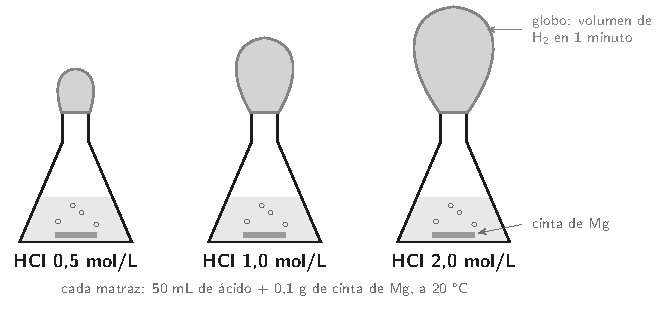
\includegraphics[max width=0.92\linewidth,max height=8.5cm]{qui/hab_globos}
\end{center}
  

En el montaje, un grupo pone 0,1 g de magnesio en 50 mL de HCl de tres concentraciones y mide cuánto se infla el globo con el H\textsubscript{2} formado en 1 minuto.

 
\begin{center}\small
\begin{tabularx}{\linewidth}{@{}>{\raggedright\arraybackslash\hsize=0.50\hsize}X>{\raggedright\arraybackslash\hsize=1.25\hsize}X>{\raggedright\arraybackslash\hsize=1.25\hsize}X@{}}
\toprule
\textbf{Variable} & \textbf{Cómo reconocerla} & \textbf{En el montaje} \\
\midrule
\textbf{Independiente} & La que el investigador \textbf{cambia a propósito} (la causa). & Concentración de HCl \\
\textbf{Dependiente} & La que se \textbf{mide} como respuesta (el efecto). & Volumen de H\textsubscript{2} (tamaño del globo) \\
\textbf{Controladas} & Las que se dejan \textbf{iguales} para que no influyan. & Masa de Mg, volumen de ácido, temperatura, tiempo \\
\bottomrule
\end{tabularx}
\end{center}
  
\gatotip[\gatoblanco]{\textbf{Truco de la frase.} Arma la frase «el efecto de \textbf{[independiente]} sobre \textbf{[dependiente]}». Aquí: «el efecto de la concentración de HCl sobre el volumen de H\textsubscript{2}». Si la frase no tiene sentido, cambiaste el orden.}
 
\begin{ejemplo}[{Ejemplo resuelto}] Se hacen reaccionar 1,5 g y 3 g del elemento Y con 2 g del elemento X, y se masa el compuesto formado.\par · Cambia a propósito: la masa de Y \ensuremath{\rightarrow} \textbf{independiente}.\par · Se mide al final: la masa de compuesto \ensuremath{\rightarrow} \textbf{dependiente}.\par · Siempre 2 g: la masa de X \ensuremath{\rightarrow} \textbf{controlada}.\end{ejemplo}
 
\begin{ojo}[{Ojo con las tablas}] La variable independiente suele ir en la primera columna y la dependiente en la última, pero no siempre. Pregúntate: ¿qué decidió el investigador \textbf{antes} de medir?\end{ojo}
\subsection{Grupo control, procedimiento e instrumentos}
El \textbf{grupo control} es el ensayo de comparación: igual a los demás, pero \textbf{sin} el factor que se estudia. Si quieres probar que el MnO\textsubscript{2} acelera la descomposición del H\textsubscript{2}O\textsubscript{2}, necesitas un tubo con H\textsubscript{2}O\textsubscript{2} y MnO\textsubscript{2} y otro tubo igual, con el mismo H\textsubscript{2}O\textsubscript{2} y a la misma temperatura, pero sin MnO\textsubscript{2}. Sin ese tubo no sabes si el MnO\textsubscript{2} hizo algo.

 

\textbf{Compara solo ensayos que se diferencian en una cosa.}

 
\begin{center}\small
\begin{tabular}{@{}lll@{}}
\toprule
\textbf{Ensayo} & \textbf{Temperatura} & \textbf{Azúcar} \\
\midrule
1 & 20 °C & granulada \\
2 & 40 °C & granulada \\
3 & 40 °C & flor (polvo) \\
\bottomrule
\end{tabular}
\end{center}
 

· 1 y 2: solo cambia la temperatura \ensuremath{\rightarrow} sirven para estudiar la temperatura.\par · 2 y 3: solo cambia el tamaño del grano \ensuremath{\rightarrow} sirven para el tamaño.\par · 1 y 3: cambian dos cosas \ensuremath{\rightarrow} no sirven: no sabrías cuál causó la diferencia.

  
\begin{clave}[{Instrumentos según la variable}] \begin{center}\small
\begin{tabularx}{\linewidth}{@{}>{\raggedright\arraybackslash\hsize=0.86\hsize}X>{\raggedright\arraybackslash\hsize=1.14\hsize}X@{}}
\toprule
\textbf{Para medir\dots{}} & \textbf{se usa\dots{}} \\
\midrule
masa & balanza \\
volumen de un líquido & probeta (aproximado), pipeta o bureta (preciso) \\
volumen exacto de una solución & matraz aforado \\
volumen de un gas & jeringa de gas, probeta invertida, cilindro con émbolo \\
temperatura & termómetro \\
tiempo & cronómetro \\
presión & barómetro o manómetro \\
acidez & pHmetro o papel indicador \\
\bottomrule
\end{tabularx}
\end{center}\end{clave}
 
\begin{ojo}[{Lee bien qué variable piden}] Si un gas se calienta a presión constante y se mide cómo cambia su volumen, el termómetro mide la variable independiente; la dependiente (el volumen) se mide con un cilindro graduado con émbolo móvil.\end{ojo}
\subsection{Ley, teoría, modelo y los demás componentes}
La PAES pregunta mucho «¿a qué componente de la investigación corresponde la frase entre comillas?». Apréndete esta tabla:

 
\begin{center}\small
\begin{tabularx}{\linewidth}{@{}>{\raggedright\arraybackslash\hsize=0.50\hsize}X>{\raggedright\arraybackslash\hsize=1.25\hsize}X>{\raggedright\arraybackslash\hsize=1.25\hsize}X@{}}
\toprule
\textbf{Componente} & \textbf{Qué es} & \textbf{Ejemplo en química} \\
\midrule
\textbf{Ley} & Describe una regularidad: \textbf{qué} pasa, a menudo con una fórmula. & Ley de conservación de la masa (Lavoisier); ley de las proporciones definidas (Proust); ley de Boyle. \\
\textbf{Teoría} & Explica \textbf{por qué} pasa; está respaldada por mucha evidencia. & Teoría atómica de Dalton; teoría cinético-molecular. \\
\textbf{Modelo} & Representación simplificada para explicar o predecir. & Modelo atómico de Bohr; modelo de esferas y varillas. \\
\textbf{Objetivo} & Lo que se quiere lograr; empieza con un verbo en infinitivo. & «Determinar la concentración de ácido acético de un vinagre». \\
\textbf{Procedimiento} & Los pasos que se siguen. & «Se quemó la muestra, se masaron el CO\textsubscript{2} y el H\textsubscript{2}O formados\dots{}». \\
\textbf{Observación} & Lo que se percibe o mide directamente. & «Se forma un sólido amarillo en el fondo del tubo». \\
\textbf{Resultado} & Los datos obtenidos. & «Las muestras del mar Rojo tienen entre 42 y 46 g/L de iones». \\
\textbf{Inferencia} & Interpretación que va más allá de lo observado. & «Casi todas las partículas alfa atraviesan la lámina: el átomo es mayormente vacío». \\
\textbf{Conclusión} & Respuesta a la pregunta, apoyada en los resultados. & «Estos cristales son yodo purificado mediante el procedimiento». \\
\bottomrule
\end{tabularx}
\end{center}
  
\begin{clave}[{Pistas en el texto}] · «si\dots{}, entonces\dots{} ocurrirá», «podría doblarse»: predicción.\par · «se agregó, se calentó, se midió»: procedimiento.\par · «se obtuvo», «los valores fueron»: resultado.\par · «por lo tanto», «esto indica», «corresponde a»: conclusión o inferencia.\end{clave}
  
\begin{ojo}[{Error típico}] Creer que una teoría es «una suposición» o que con más pruebas «se convierte en ley». No: la ley dice qué pasa y la teoría explica por qué. Son cosas distintas y ninguna pasa a ser la otra.\end{ojo}
\subsection{Lo clave del tema}
\begin{center}\small
\begin{tabularx}{\linewidth}{@{}>{\raggedright\arraybackslash\hsize=0.77\hsize}X>{\raggedright\arraybackslash\hsize=1.23\hsize}X@{}}
\toprule
\textbf{Concepto} & \textbf{Lo que tienes que reconocer} \\
\midrule
Pregunta de investigación & Se responde midiendo; calza con lo que se varió y lo que se midió. \\
Hipótesis & Respuesta tentativa que relaciona la variable independiente con la dependiente. \\
Predicción & Resultado concreto esperado: «si\dots{}, entonces\dots{}». \\
Variable independiente & La que se cambia a propósito. \\
Variable dependiente & La que se mide. \\
Variables controladas & Las que se mantienen iguales. \\
Grupo control & Ensayo sin el factor estudiado, para comparar. \\
Ley / teoría / modelo & Qué pasa / por qué pasa / representación simplificada. \\
\bottomrule
\end{tabularx}
\end{center}
 
\begin{clave}[{Recuerda}] · Variable independiente: la que se decide antes; dependiente: la que se mide.\par · La hipótesis habla de la variable que cambia en el experimento.\par · Para estudiar una variable, compara ensayos que solo difieren en esa variable.\par · «El pH fue 5,2» es un resultado; la conclusión lo interpreta y responde la pregunta.\par · Cada variable se mide con su instrumento: la temperatura con termómetro, el volumen con probeta.\end{clave}
 
\begin{clave}[{Método PAES}] 1. Subraya qué se cambió, qué se midió y qué se dejó igual. 2. Con eso, nombra las tres variables. 3. Si preguntan por la hipótesis o la pregunta, elige la que relaciona exactamente esas dos variables. 4. Si preguntan por un componente, busca las pistas («si\dots{} entonces», «se obtuvo», «se agregó»). 5. Descarta las alternativas que hablan de variables que no cambiaron.\end{clave}
\begin{elejemplo}{PAES Invierno 2027, adaptada}
En la producción de litio se precipita carbonato de litio, Li\textsubscript{2}CO\textsubscript{3}, desde una solución acuosa. Como este compuesto es bastante soluble en agua, un grupo de investigadores estudia qué parámetros permiten disminuir su solubilidad. En la tabla se presentan las condiciones de cuatro ensayos:
\begin{center}\small
\begin{tabularx}{\linewidth}{@{}>{\raggedright\arraybackslash\hsize=0.39\hsize}X>{\raggedright\arraybackslash\hsize=0.69\hsize}X>{\raggedright\arraybackslash\hsize=1.20\hsize}X>{\raggedright\arraybackslash\hsize=1.72\hsize}X@{}}
\toprule
\textbf{Ensayo} & \textbf{Temperatura (°C)} & \textbf{Velocidad de agitación (rpm)} & \textbf{Concentración inicial de Li\textsubscript{2}CO\textsubscript{3} (mol/L)} \\
\midrule
\textbf{1} & 25 & 150 & 2 \\
\textbf{2} & 25 & 300 & 2 \\
\textbf{3} & 45 & 150 & 2 \\
\textbf{4} & 45 & 300 & 1 \\
\bottomrule
\end{tabularx}
\end{center}
\altslargas{Comparar los ensayos 1 y 2 permite analizar el efecto de la temperatura.}{Comparar los ensayos 2 y 4 permite analizar el efecto de la concentración.}{Comparar los ensayos 1 y 3 permite analizar el efecto de la temperatura.}{Comparar los ensayos 3 y 4 permite analizar el efecto de la velocidad de agitación.}
\solucion{\textbf{Paso 1. ¿Qué nos piden?} Elegir un par de ensayos que sirva para estudiar el efecto de \textbf{un} parámetro. La regla de oro: dos ensayos sirven para estudiar una variable solo si se diferencian \textbf{únicamente} en esa variable. Así, si el resultado cambia, sabemos qué lo causó.

\textbf{Paso 2. Ensayos 1 y 2.} Temperatura: 25 y 25 (igual). Agitación: 150 y 300 (cambia). Concentración: 2 y 2 (igual). Solo cambia la agitación: este par sirve para la \textbf{agitación}, no para la temperatura.

\textbf{Paso 3. Ensayos 2 y 4.} Temperatura: 25 y 45 (cambia). Agitación: 300 y 300 (igual). Concentración: 2 y 1 (cambia). Cambian dos parámetros a la vez: este par no sirve para nada, porque no sabríamos cuál causó la diferencia.

\textbf{Paso 4. Ensayos 1 y 3.} Temperatura: 25 y 45 (cambia). Agitación: 150 y 150 (igual). Concentración: 2 y 2 (igual). Solo cambia la temperatura: este par sirve para estudiar la \textbf{temperatura}. \ding{52}

\textbf{Paso 5. Ensayos 3 y 4.} Temperatura: 45 y 45 (igual). Agitación: 150 y 300 (cambia). Concentración: 2 y 1 (cambia). Cambian dos parámetros: no sirve.

\textbf{Respuesta:} comparar los ensayos 1 y 3 permite analizar el efecto de la temperatura.

\textbf{Comprobación:} en los ensayos 1 y 3 la temperatura es la variable independiente y la agitación (150 rpm) y la concentración inicial (2 mol/L) son variables controladas. Es justo el diseño que se necesita.

\textbf{¿Por qué no las otras?} «1 y 2 para la temperatura» se equivoca de variable: en ese par la temperatura es igual (25 °C) y lo único que cambia es la agitación. «2 y 4 para la concentración» y «3 y 4 para la agitación» eligen pares en los que cambian dos parámetros a la vez; cualquier diferencia en la solubilidad podría deberse a cualquiera de los dos.

\textbf{\color{cienciaD}Para recordar.} Para estudiar una variable, compara solo ensayos que se diferencian únicamente en esa variable.}{C}
\end{elejemplo}

%% =====================================================================
%% qui_hab_evidencia
\section[Procesar y analizar la evidencia]{Procesar y analizar la evidencia}
\modcomun\ \ {\color{gris}\itshape Leer tablas y gráficos de experimentos químicos, reconocer tendencias y relaciones directas, inversas y proporcionales, hacer predicciones e inferencias y sacar conclusiones que se sostienen con los datos.\par}
\subsection{Leer una tabla de datos}
Antes de mirar las alternativas, lee la tabla en cuatro pasos:

 

\textbf{Paso 1. Encabezados y unidades.} ¿Qué mide cada columna? ¿En qué unidad?

 

\textbf{Paso 2. ¿Qué cambia y qué se mide?} Identifica la variable independiente y la dependiente.

 

\textbf{Paso 3. Recorre en orden.} Sigue la columna que crece y mira qué hace la otra: ¿sube, baja o queda igual?

 

\textbf{Paso 4. Revisa todas las filas.} Una tendencia vale solo si se cumple en todas.

 
\begin{center}\small
\begin{tabularx}{\linewidth}{@{}>{\raggedright\arraybackslash\hsize=0.56\hsize}X>{\raggedright\arraybackslash\hsize=1.40\hsize}X>{\raggedright\arraybackslash\hsize=1.21\hsize}X>{\raggedright\arraybackslash\hsize=0.84\hsize}X@{}}
\toprule
\textbf{Compuesto} & \textbf{Temperatura de ebullición (°C)} & \textbf{Temperatura de fusión (°C)} & \textbf{Propiedad X (u.a.)} \\
\midrule
NaF & 1705 & 990 & 2,21 \\
NaCl & 1413 & 801 & 2,81 \\
NaBr & 1390 & 755 & 2,97 \\
NaI & 1300 & 651 & 3,23 \\
\bottomrule
\end{tabularx}
\end{center}
  
\begin{ejemplo}[{Ejemplo resuelto}] En la tabla, la propiedad X crece de arriba hacia abajo: 2,21 \ensuremath{\rightarrow} 2,81 \ensuremath{\rightarrow} 2,97 \ensuremath{\rightarrow} 3,23. Mientras tanto, la temperatura de ebullición baja (1705 \ensuremath{\rightarrow} 1300) y la de fusión también (990 \ensuremath{\rightarrow} 651).\par Relaciones correctas:\par · «La temperatura de ebullición \textbf{disminuye} al aumentar la propiedad X».\par · «La temperatura de fusión \textbf{aumenta} al disminuir la propiedad X» (es lo mismo, leído al revés).\end{ejemplo}
 
\begin{ojo}[{La trampa del «al disminuir»}] «La temperatura de fusión disminuye al disminuir X» es \textbf{falsa}: si X baja, la temperatura sube. Cuando una alternativa recorre la tabla al revés, recórrela tú también al revés antes de responder.\end{ojo}
\subsection{Leer un gráfico}
\begin{center}
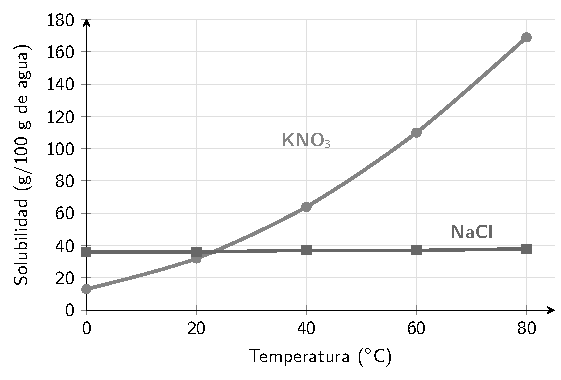
\includegraphics[max width=0.92\linewidth,max height=8.5cm]{qui/hab_solubilidad}
\end{center}
 

\textbf{Paso 1. Ejes.} Eje horizontal: temperatura (°C), la variable independiente. Eje vertical: solubilidad, en gramos de sal por 100 g de agua, la variable dependiente.

 

\textbf{Paso 2. Escala.} Cada línea horizontal vale 20 g; cada vertical, 20 °C.

 

\textbf{Paso 3. Lee puntos.} A 60 °C se disuelven como máximo 110 g de KNO\textsubscript{3} en 100 g de agua. A 20 °C, solo 32 g.

 

\textbf{Paso 4. Compara curvas.} Las curvas se cruzan cerca de 22 °C: por debajo de esa temperatura el NaCl es más soluble; por encima, el KNO\textsubscript{3}.

  
\begin{clave}[{La pendiente cuenta la historia}] La curva del KNO\textsubscript{3} sube mucho: su solubilidad depende fuertemente de la temperatura. La del NaCl es casi plana (36 a 38 g): casi no cambia.\end{clave}
 
\begin{ejemplo}[{Ejemplo resuelto}] Una solución saturada de KNO\textsubscript{3} en 100 g de agua a 60 °C se enfría hasta 40 °C. ¿Cuánto KNO\textsubscript{3} cristaliza?\par \textbf{Paso 1.} A 60 °C hay disueltos 110 g.\par \textbf{Paso 2.} A 40 °C caben solo 64 g.\par \textbf{Paso 3.} Cristaliza la diferencia: $110 - 64 = 46$ g.\end{ejemplo}
 
\begin{ojo}[{Ojo con la cantidad de agua}] El gráfico es «por 100 g de agua». Con 50 g de agua cabe la mitad: a 60 °C, 55 g de KNO\textsubscript{3}, no 110 g.\end{ojo}
\subsection{Relaciones entre variables}
\begin{center}
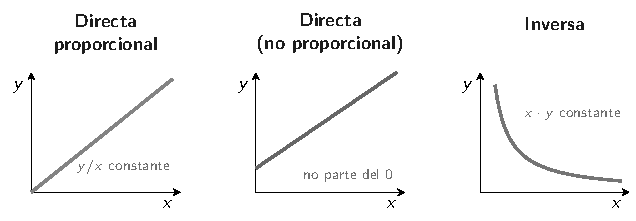
\includegraphics[max width=0.92\linewidth,max height=8.5cm]{qui/hab_relaciones}
\end{center}
  
\begin{center}\small
\begin{tabularx}{\linewidth}{@{}>{\raggedright\arraybackslash\hsize=0.71\hsize}X>{\raggedright\arraybackslash\hsize=1.14\hsize}X>{\raggedright\arraybackslash\hsize=1.14\hsize}X@{}}
\toprule
\textbf{Relación} & \textbf{Qué pasa} & \textbf{Cómo comprobarla} \\
\midrule
Directa & Si una aumenta, la otra también. & Ambas columnas suben juntas. \\
Directamente proporcional & Si una se duplica, la otra se duplica. & El cociente $y/x$ es constante; el gráfico es una recta que pasa por el origen. \\
Inversa & Si una aumenta, la otra disminuye. & Una columna sube y la otra baja. \\
Inversamente proporcional & Si una se duplica, la otra se reduce a la mitad. & El producto $x\cdot y$ es constante. \\
\bottomrule
\end{tabularx}
\end{center}
  
\begin{ejemplo}[{Ejemplo resuelto}] Un gas a temperatura constante:
\begin{center}\small
\begin{tabular}{@{}lll@{}}
\toprule
\textbf{Presión (atm)} & \textbf{Volumen (L)} & \textbf{$P\cdot V$} \\
\midrule
1 & 12 & 12 \\
2 & 6 & 12 \\
3 & 4 & 12 \\
\bottomrule
\end{tabular}
\end{center}
 El producto es siempre 12: el volumen es \textbf{inversamente proporcional} a la presión (ley de Boyle).\end{ejemplo}
 
\begin{ojo}[{No todo lo directo es proporcional}] La temperatura de ebullición de los alcanos sube con el número de carbonos, pero el propano hierve a \ensuremath{-}42 °C: el gráfico no pasa por el origen. Es una relación directa, no proporcional. Lo mismo con las inversas: que una baje cuando la otra sube no basta; el producto tiene que ser constante.\end{ojo}
\subsection{Tendencias: interpolar y predecir}
Una \textbf{tendencia} es el patrón que siguen los datos. Con ella se puede estimar un valor que no se midió.

 
\begin{itemize}
  \item \textbf{Interpolar}: estimar un valor \textbf{dentro} del rango medido. Es bastante seguro.
  \item \textbf{Extrapolar}: estimar \textbf{fuera} del rango medido. Es arriesgado, y solo vale para valores cercanos.
\end{itemize}
 
\begin{center}\small
\begin{tabular}{@{}lll@{}}
\toprule
\textbf{Alcano lineal} & \textbf{N.º de C} & \textbf{Temperatura de ebullición (°C)} \\
\midrule
Pentano & 5 & 36 \\
Hexano & 6 & 69 \\
Heptano & 7 & 98 \\
Octano & 8 & 126 \\
\bottomrule
\end{tabular}
\end{center}
 

Las diferencias son 33, 29 y 28 °C: cada carbono extra sube la temperatura de ebullición en unos 30 °C, y el salto se achica poco a poco. Para el nonano (9 C) se espera algo más de 150 °C. El valor real es 151 °C.

  
\begin{ejemplo}[{Ejemplo resuelto: predecir con dos tendencias}] \begin{center}\small
\begin{tabular}{@{}llll@{}}
\toprule
\textbf{Lineal} & \textbf{°C} & \textbf{Con una ramificación} & \textbf{°C} \\
\midrule
Pentano & 36,1 & 2-metilbutano & 27,8 \\
Hexano & 68,7 & 2-metilpentano & 60,3 \\
Heptano & 98,4 & 2-metilhexano & ? \\
\bottomrule
\end{tabular}
\end{center}
\textbf{Paso 1.} La ramificación baja la temperatura de ebullición en unos 8,4 °C: $36{,}1 - 27{,}8 = 8{,}3$ y $68{,}7 - 60{,}3 = 8{,}4$.\par \textbf{Paso 2.} Para el 2-metilhexano: $98{,}4 - 8{,}4 = 90{,}0$ °C. El valor real es 90,0 °C.\end{ejemplo}
 
\begin{ojo}[{No extrapoles lejos}] Que tres datos bajen no significa que sigan bajando hasta cero ni que sigan igual a 200 °C. La conclusión vale para el rango estudiado.\end{ojo}
\subsection{De los datos a la conclusión}
Una \textbf{conclusión} o \textbf{inferencia} correcta cumple tres condiciones:

 
\begin{itemize}
  \item \textbf{Sale de los datos.} Lo que afirma se puede ver en la tabla o el gráfico.
  \item \textbf{Habla solo de lo que se midió.} Las mismas variables y el mismo rango; si se midió a 1 y a 8 horas, vale «en los dos tiempos estudiados».
  \item \textbf{No agrega cosas.} Ni síntomas, ni «siempre», ni «todas las sustancias», ni causas que el experimento no puso a prueba.
\end{itemize}
 
\begin{ejemplo}[{Ejemplo resuelto: reactivo limitante}] BaCl\textsubscript{2} + Na\textsubscript{2}SO\textsubscript{4} \ensuremath{\rightarrow} BaSO\textsubscript{4} + 2 NaCl, todo en razón 1 : 1.
\begin{center}\small
\begin{tabular}{@{}llll@{}}
\toprule
\textbf{Tubo} & \textbf{BaCl\textsubscript{2} (mol)} & \textbf{Na\textsubscript{2}SO\textsubscript{4} (mol)} & \textbf{BaSO\textsubscript{4} (mol)} \\
\midrule
1 & 0,0001 & 0,0009 & 0,0001 \\
3 & 0,0003 & 0,0007 & 0,0003 \\
5 & 0,0005 & 0,0005 & 0,0005 \\
\bottomrule
\end{tabular}
\end{center}
 El precipitado coincide siempre con el BaCl\textsubscript{2}, que es el que está en menor cantidad: la cantidad de precipitado depende del \textbf{reactivo limitante}, el BaCl\textsubscript{2}.\end{ejemplo}
  
\begin{ejemplo}[{Ejemplo resuelto: proporción constante}] Dos ensayos combinan 0,25 mol de Y con 0,50 mol de X, y 0,50 mol de Y con 1,00 mol de X. En ambos, $\dfrac{n_X}{n_Y} = 2$: X e Y se combinan en la misma proporción (2 : 1) en los dos ensayos. Es la ley de las proporciones definidas.\end{ejemplo}
 
\begin{ojo}[{Palabras sospechosas}] «Siempre», «todos», «demuestra definitivamente», «cualquier tipo de\dots{}», «se vuelve irreversible». Si la tabla no lo muestra, la alternativa es falsa aunque suene científica.\end{ojo}
 
\begin{ojo}[{Correlación no es causa}] Que dos variables cambien juntas no prueba que una cause la otra, salvo que el experimento haya cambiado una y controlado todo lo demás.\end{ojo}
\subsection{Cálculos rápidos con los datos}
Muchas preguntas de evidencia piden comparar \textbf{cocientes}, no los números de la tabla. Sin calculadora, simplifica las fracciones.

 
\begin{ejemplo}[{Ejemplo resuelto: eficiencia}] Cuatro métodos producen hidrógeno a partir de agua. ¿Cuál es más eficiente?
\begin{center}\small
\begin{tabular}{@{}llll@{}}
\toprule
\textbf{Método} & \textbf{Agua usada (L)} & \textbf{H\textsubscript{2} producido (mol)} & \textbf{mol por litro} \\
\midrule
1 & 10 & 0,8 & 0,08 \\
2 & 12 & 1,0 & 0,083 \\
3 & 15 & 1,5 & 0,10 \\
4 & 25 & 1,8 & 0,072 \\
\bottomrule
\end{tabular}
\end{center}
 El método 4 produce más hidrógeno en total, pero gasta mucha más agua. Por cada litro, el más eficiente es el \textbf{método 3}.\end{ejemplo}
  
\begin{ejemplo}[{Ejemplo resuelto: porcentaje en masa}] Al quemar 0,70 g de hierro se forma 1,00 g de óxido. Porcentaje de hierro: $\dfrac{0{,}70}{1{,}00}\cdot 100 = 70\%$. Si otro ensayo da 7,78 g de hierro en 10,00 g de óxido, el porcentaje es 77,8 \%: se formó un óxido distinto.\end{ejemplo}
 
\gatotip[\gatonaranjo]{\textbf{Trucos sin calculadora.} · Para comparar $\dfrac{0{,}8}{10}$ con $\dfrac{1{,}0}{12}$, multiplica en cruz: $0{,}8\cdot 12 = 9{,}6$ y $1{,}0\cdot 10 = 10$. Como $9{,}6 < 10$, la primera fracción es menor.\par · Para un porcentaje, lleva el denominador a 100: $\dfrac{3{,}89}{5} = \dfrac{77{,}8}{100} = 77{,}8\%$.}
 
\begin{ojo}[{Error típico}] Elegir la fila con el número más grande. «Más eficiente», «mayor rendimiento» y «mayor porcentaje» piden un cociente, no un total.\end{ojo}
\subsection{Lo clave del tema}
\begin{center}\small
\begin{tabularx}{\linewidth}{@{}>{\raggedright\arraybackslash\hsize=0.95\hsize}X>{\raggedright\arraybackslash\hsize=1.05\hsize}X@{}}
\toprule
\textbf{Si te piden\dots{}} & \textbf{Haz esto} \\
\midrule
Una relación o tendencia & Recorre la variable que crece y mira qué hace la otra; revisa todas las filas. \\
Saber si es proporcional & Directa: cociente constante, recta por el origen. Inversa: producto constante. \\
Leer un gráfico & Ejes, unidades y escala antes de leer un punto. \\
Una predicción & Sigue la tendencia (diferencias entre valores seguidos), sin extrapolar lejos. \\
Una conclusión o inferencia & Que salga de los datos, hable solo de lo medido y no agregue nada. \\
Eficiencia, rendimiento o porcentaje & Calcula un cociente para cada fila y compara. \\
\bottomrule
\end{tabularx}
\end{center}
 
\begin{clave}[{Recuerda}] · En una relación inversa, cuando una variable disminuye, la otra aumenta.\par · Una relación es proporcional solo si el cociente entre las variables es constante.\par · Las curvas de solubilidad se leen por 100 g de agua: si caben 110 g de KNO\textsubscript{3} en 100 g, en 50 g caben 55 g.\par · La conclusión se limita a lo estudiado: «en el rango estudiado, la solubilidad del KNO\textsubscript{3} aumenta con la temperatura».\par · La eficiencia se compara con lo producido por unidad de lo gastado.\end{clave}
 
\begin{clave}[{Método PAES}] 1. Lee encabezados, ejes y unidades. 2. Identifica qué cambió y qué se midió. 3. Describe en tu cabeza la tendencia antes de leer las alternativas. 4. Si hay números, calcula el cociente, la diferencia o el producto que corresponda. 5. Descarta lo que no sale de los datos, lo que generaliza y lo que habla de variables que no se midieron.\end{clave}
\begin{elejemplo}{PAES Invierno 2027, adaptada}
Un estudiante encuentra en un libro la temperatura de ebullición, a 1 atm, de un conjunto de alcanos de cadena lineal, no ramificados, cuyos átomos de carbono están unidos entre sí solo por enlaces simples C--C. Con esa información elabora el siguiente gráfico:
\begin{center}
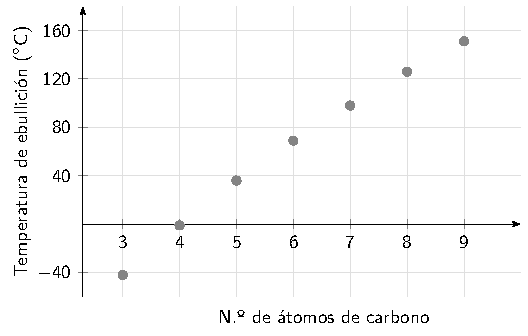
\includegraphics[max width=0.92\linewidth,max height=8.5cm]{qui/hab_alcanos}
\end{center}
\altslargas{A medida que aumenta el número de átomos de carbono, la temperatura de ebullición es menor que cero.}{A medida que disminuye el número de átomos de carbono, la temperatura de ebullición disminuye.}{La temperatura de ebullición es directamente proporcional al número de átomos de carbono.}{La temperatura de ebullición se mantiene constante para los alcanos con más de 7 átomos de carbono.}
\solucion{\textbf{Paso 1. ¿Qué nos piden?} La afirmación que describe correctamente la tendencia del gráfico. Primero leemos el gráfico y después revisamos cada alternativa.

\textbf{Paso 2. Lee los ejes.} Eje horizontal: número de átomos de carbono (3 a 9). Eje vertical: temperatura de ebullición en °C. Cada línea vale 40 °C.

\textbf{Paso 3. Lee los puntos.} 3 C: unos \ensuremath{-}42 °C. 4 C: casi 0 °C. 5 C: 36 °C. 6 C: 69 °C. 7 C: 98 °C. 8 C: 126 °C. 9 C: 151 °C.

\textbf{Paso 4. Describe la tendencia.} De izquierda a derecha, los puntos siempre suben: al aumentar el número de carbonos aumenta la temperatura de ebullición. Leído al revés, al disminuir el número de carbonos, la temperatura de ebullición disminuye. Es una relación directa.

\textbf{Paso 5. Revisa la relación con números.} ¿Es proporcional? Si lo fuera, el cociente temperatura/carbonos sería constante y la recta pasaría por el origen. Pero con 3 C el valor es negativo (\ensuremath{-}42 °C) y con 4 C es casi 0 °C: no es proporcional.

\textbf{Respuesta:} a medida que disminuye el número de átomos de carbono, la temperatura de ebullición disminuye.

\textbf{Comprobación:} recorre el gráfico de derecha a izquierda: 151 \ensuremath{\rightarrow} 126 \ensuremath{\rightarrow} 98 \ensuremath{\rightarrow} 69 \ensuremath{\rightarrow} 36 \ensuremath{\rightarrow} \ensuremath{-}1 \ensuremath{\rightarrow} \ensuremath{-}42. Siempre baja. \ding{52} La explicación química: con más carbonos la molécula es más grande, las fuerzas entre moléculas son mayores y cuesta más separarlas.

\textbf{¿Por qué no las otras?} «Es menor que cero» es falsa: solo el propano (y, apenas, el butano) quedan bajo cero; desde 5 C todos están sobre cero. «Directamente proporcional» confunde relación directa con proporcional: al duplicar los carbonos de 4 a 8, la temperatura no se duplica (pasa de unos 0 °C a 126 °C), y el gráfico no pasa por el origen. «Se mantiene constante sobre 7 C» es falsa: de 7 a 9 C sigue subiendo, de 98 a 151 °C.

\textbf{\color{cienciaD}Para recordar.} Describe la tendencia en las dos direcciones y no confundas una relación directa con una proporcional.}{B}
\end{elejemplo}

%% =====================================================================
%% qui_hab_evaluar
\section[Evaluar y comunicar una investigación]{Evaluar y comunicar una investigación}
\modcomun\ \ {\color{gris}\itshape Juzgar la validez y la confiabilidad de un experimento químico, decidir si una conclusión se sostiene con los datos, reconocer limitaciones del diseño y cómo mejorarlo, la reproducibilidad, los alcances tecnológicos y el recurso adecuado para comunicar resultados.\par}
\subsection{Validez y confiabilidad}
\textbf{Validez:} la investigación mide de verdad lo que dice medir y su diseño permite sacar la conclusión. Falla cuando no se controlaron variables, cuando falta un grupo control o cuando se mide otra cosa.

 

\textbf{Confiabilidad:} al repetir las mediciones se obtienen resultados parecidos. Depende de cuántas veces se repite, del tamaño de la muestra y de la precisión de los instrumentos.

 

\textbf{Precisión y exactitud.} Mediciones \textbf{precisas} son cercanas entre sí. Mediciones \textbf{exactas} son cercanas al valor real. Se puede ser preciso sin ser exacto, por ejemplo con una balanza mal calibrada que siempre marca 0,5 g de más.

 
\begin{center}\small
\begin{tabular}{@{}ll@{}}
\toprule
\textbf{Instrumento} & \textbf{Lectura típica} \\
\midrule
Balanza analítica & 0,001 g \\
Bureta, pipeta aforada & 0,05 mL \\
Probeta de 100 mL & 1 mL \\
Vaso de precipitados & solo aproximado \\
\bottomrule
\end{tabular}
\end{center}
  
\begin{ejemplo}[{Ejemplo resuelto}] Unos estudiantes miden la densidad de muestras de cobre puro (valor de referencia 8,96 g/cm\textsuperscript{3}). Masan con una balanza de tres decimales (8,801 g), pero leen el volumen en una probeta como 1,0, 1,5 o 2,0 cm\textsuperscript{3}. Las densidades salen entre 8,4 y 9,5 g/cm\textsuperscript{3}.\par \textbf{¿Qué perjudica la confiabilidad?} La medición del volumen: es mucho menos precisa que la de la masa y, como el volumen es pequeño, un error de 0,1 cm\textsuperscript{3} cambia la densidad en casi un 10 \%.\end{ejemplo}
 
\begin{ojo}[{Lo que no es el problema}] Usar un valor de referencia para comparar no daña la confiabilidad: es justamente lo que permite evaluar el resultado. Tampoco el origen de las muestras, si todas son del mismo material.\end{ojo}
\subsection{¿La conclusión se sostiene con los datos?}
Para evaluar una conclusión, revisa esta lista:

 

\textbf{1. ¿Responde la pregunta u objetivo?}

 

\textbf{2. ¿Habla solo de las variables medidas y del rango estudiado?}

 

\textbf{3. ¿El diseño permite distinguir?} Si se quiere mostrar que un reactivo «diferencia A de B», hay que probarlo con A \textbf{y} con B.

 

\textbf{4. ¿Se controlaron las demás variables?} Si cambiaron dos cosas a la vez, no se puede atribuir el efecto a una sola.

 

\textbf{5. ¿Hay repeticiones suficientes?} Un solo ensayo por condición da una conclusión débil.

  
\begin{ejemplo}[{Ejemplo resuelto}] Un estudiante afirma: «el KMnO\textsubscript{4} sirve para diferenciar alquenos de aldehídos». Prueba el KMnO\textsubscript{4} con seis aldehídos distintos y todos reaccionan.\par \textbf{Evaluación:} el procedimiento está mal planteado porque \textbf{solo usa aldehídos}. Sin probar alquenos, no hay con qué comparar. Los datos pueden estar bien medidos; lo que falla es el diseño. (De hecho, los alquenos también reaccionan con KMnO\textsubscript{4}).\end{ejemplo}
 
\begin{ojo}[{Error típico}] Pensar que «diseño incorrecto» significa «datos con errores». Son cosas distintas: un diseño puede ser incapaz de responder la pregunta aunque cada medición sea perfecta.\end{ojo}
\subsection{Limitaciones del diseño y cómo mejorarlo}
\begin{center}\small
\begin{tabularx}{\linewidth}{@{}>{\raggedright\arraybackslash\hsize=0.99\hsize}X>{\raggedright\arraybackslash\hsize=1.01\hsize}X@{}}
\toprule
\textbf{Limitación} & \textbf{Mejora} \\
\midrule
Un solo ensayo por condición & Repetir y promediar. \\
Falta un grupo control & Agregar un ensayo igual pero sin el factor estudiado. \\
Cambian dos variables a la vez & Cambiar solo la variable independiente. \\
La variable independiente casi no varía & Usar valores realmente distintos, en un rango amplio. \\
Instrumento poco preciso & Usar uno más preciso (pipeta en vez de vaso de precipitados). \\
Muestras distintas entre ensayos & Usar la misma cantidad y el mismo tipo de muestra. \\
\bottomrule
\end{tabularx}
\end{center}
  
\begin{ejemplo}[{Ejemplo resuelto}] Para encontrar la concentración de sal mínima que hace flotar un huevo, unos estudiantes preparan 5 g de sal en 200 cm\textsuperscript{3}, 10 g en 400 cm\textsuperscript{3} y 15 g en 500 cm\textsuperscript{3} (no flota), y 50 g en 1000 cm\textsuperscript{3} (flota).\par \textbf{Paso 1.} Calcula las concentraciones: 0,025; 0,025; 0,03 y 0,05 g/cm\textsuperscript{3}.\par \textbf{Paso 2.} Los tres primeros ensayos son casi la misma solución: no aportan información nueva.\par \textbf{Mejora:} preparar soluciones con concentraciones distintas entre sí, en pasos pequeños entre 0,03 y 0,05 g/cm\textsuperscript{3}.\end{ejemplo}
 
\begin{ojo}[{La mejora tiene que apuntar al objetivo}] Repetir el último ensayo o cambiar el huevo no ayuda a encontrar la concentración mínima. Busca la alternativa que corrige el defecto que impide responder la pregunta.\end{ojo}
\subsection{Replicabilidad y reproducibilidad}
Un procedimiento es \textbf{replicable} si está descrito con tanto detalle que otra persona puede repetirlo. Un resultado es \textbf{reproducible} si al repetir el procedimiento se obtiene el mismo resultado.

 

Para decidir qué se puede cambiar sin afectar la reproducibilidad, distingue dos tipos de propiedades:

 
\begin{itemize}
  \item \textbf{Intensivas:} no dependen de cuánta muestra hay. Densidad, concentración, temperatura de ebullición, porcentaje en masa, color.
  \item \textbf{Extensivas:} dependen de la cantidad. Masa, volumen, cantidad de sustancia.
\end{itemize}
 

Si el resultado es una propiedad intensiva, se puede usar \textbf{otra cantidad de la misma muestra} y el resultado debe ser el mismo.

  
\begin{ejemplo}[{Ejemplo resuelto}] Un laboratorio analiza 100 mL de un vinagre y obtiene 5 \% m/v de ácido acético. ¿Cómo se comprueba ese resultado?\par · Repetir el análisis con 50 mL del \textbf{mismo} vinagre: la concentración no depende del volumen analizado, así que debe dar 5 \% m/v. \ding{52}\par · Usar otro vinagre, diluir con agua o evaporar: cambia la muestra y cambia el resultado. \ding{56}\end{ejemplo}
 
\begin{ojo}[{Lo que sí afecta}] Cambiar la sustancia, la temperatura, la presión o la propiedad medida cambia el resultado. La densidad de un aceite a 38 °C no es la misma que a 49 °C.\end{ojo}
\subsection{Alcances y aplicaciones tecnológicas}
El temario también pide evaluar \textbf{cómo una investigación contribuye a la tecnología} y qué \textbf{alcance} tienen sus resultados.

 

El alcance de una investigación se limita a sus condiciones: la sustancia, el rango de valores, el tipo de muestra y el ambiente en que se hizo. Una buena alternativa usa verbos prudentes («podría mejorar», «en condiciones similares») y se apoya en los datos.

 
\begin{center}\small
\begin{tabularx}{\linewidth}{@{}>{\raggedright\arraybackslash\hsize=1.00\hsize}X>{\raggedright\arraybackslash\hsize=1.00\hsize}X@{}}
\toprule
\textbf{Investigación} & \textbf{Aporte tecnológico} \\
\midrule
Electrólisis del agua con energía renovable & Hidrógeno verde como combustible y forma de almacenar energía. \\
Solubilidad del Li\textsubscript{2}CO\textsubscript{3} según la temperatura & Mejor recuperación de litio para baterías. \\
Moléculas orgánicas con muchos enlaces pi & Celdas solares orgánicas y semiconductores. \\
Química verde: síntesis en menos etapas & Procesos industriales con menos residuos. \\
\bottomrule
\end{tabularx}
\end{center}
  
\begin{ejemplo}[{Ejemplo resuelto}] Unos investigadores prueban dos fármacos, Dox y Cur, en células de cáncer de estómago. La mayor muerte de células cancerosas (cerca de 80 \%) se logra con una razón en mol Dox : Cur de 2 : 1, y subir la dosis total no la mejora.\par \textbf{Alcance razonable:} «una dosis con el doble de Dox que de Cur, en cantidad de sustancia, \textbf{podría} mejorar el tratamiento del cáncer de estómago».\par \textbf{Alcance exagerado:} «servirá contra todos los tipos de cáncer» o «más dosis siempre es mejor».\end{ejemplo}
 
\begin{ojo}[{Error típico}] Extender un resultado de laboratorio a cualquier condición: otro tipo de célula, otra fuente de agua, otra temperatura. Los datos solo respaldan lo que se probó.\end{ojo}
\subsection{Comunicar: el recurso adecuado}
\begin{center}
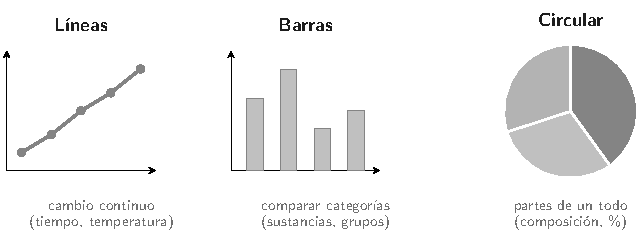
\includegraphics[max width=0.92\linewidth,max height=8.5cm]{qui/hab_graficos}
\end{center}
  
\begin{center}\small
\begin{tabularx}{\linewidth}{@{}>{\raggedright\arraybackslash\hsize=1.16\hsize}X>{\raggedright\arraybackslash\hsize=0.84\hsize}X@{}}
\toprule
\textbf{Objetivo} & \textbf{Recurso} \\
\midrule
Mostrar cómo cambia una variable continua (tiempo, temperatura, concentración) & Gráfico de líneas o de puntos \\
Comparar categorías (sustancias, marcas, métodos) & Gráfico de barras \\
Mostrar las partes de un total (composición en \%) & Gráfico circular \\
Entregar valores exactos o muchas variables & Tabla \\
Mostrar la forma de una molécula en el espacio & Modelo de esferas y varillas \\
Mostrar los grupos funcionales & Fórmula estructural \\
\bottomrule
\end{tabularx}
\end{center}
  
\begin{clave}[{Qué va en cada eje}] La variable independiente va en el eje horizontal y la dependiente en el vertical. Ejemplo: «a medida que el electrón está más lejos del núcleo, se necesita menos energía para separarlo». Eje horizontal: distancia al núcleo. Eje vertical: energía.\end{clave}
 
\begin{ojo}[{Moléculas en 3D}] Dos formas de una molécula con los mismos átomos, pero ordenados distinto en el espacio, tienen la misma fórmula molecular y la misma fórmula empírica. Para distinguirlas se necesita un modelo tridimensional, como el de esferas y varillas.\end{ojo}
 
\begin{clave}[{Tablas coherentes}] La composición porcentual de un compuesto puro es la misma en cualquier muestra: 5 g o 25 g de H\textsubscript{3}PO\textsubscript{4} tienen los mismos porcentajes de H, P y O. Una tabla que muestre porcentajes distintos para dos muestras del mismo compuesto está mal.\end{clave}
\subsection{Lo clave del tema}
\begin{center}\small
\begin{tabularx}{\linewidth}{@{}>{\raggedright\arraybackslash\hsize=0.64\hsize}X>{\raggedright\arraybackslash\hsize=1.36\hsize}X@{}}
\toprule
\textbf{Concepto} & \textbf{Pregunta que te haces} \\
\midrule
Validez & ¿El diseño permite responder la pregunta? ¿Se controlaron las variables? \\
Confiabilidad & ¿Hubo repeticiones? ¿Los instrumentos son precisos? \\
Conclusión válida & ¿Sale de los datos y no va más allá? \\
Mejora del diseño & ¿Qué defecto impide cumplir el objetivo y cómo se corrige? \\
Reproducibilidad & ¿Lo que se cambia altera una propiedad intensiva del sistema? \\
Alcance tecnológico & ¿La aplicación se limita a las condiciones estudiadas? \\
Comunicar & ¿Qué recurso muestra mejor lo que quiero mostrar? \\
\bottomrule
\end{tabularx}
\end{center}
 
\begin{clave}[{Recuerda}] · Para afirmar que un reactivo diferencia dos tipos de compuestos, hay que probarlo con ambos.\par · Los datos pueden ser correctos aunque el diseño no responda la pregunta.\par · Densidad y concentración son intensivas: no cambian con la cantidad de muestra.\par · El alcance de una conclusión se limita a condiciones similares a las estudiadas.\par · Las partes de un todo, como la composición del aire, se muestran en un gráfico circular.\end{clave}
 
\begin{clave}[{Método PAES}] 1. Escribe en una línea el objetivo de la investigación. 2. Revisa si el diseño cambia solo la variable independiente, tiene control y repeticiones. 3. Para una conclusión o un alcance, descarta lo que afirma más de lo medido. 4. Para una mejora, elige la que corrige el defecto que impide cumplir el objetivo. 5. Para comunicar, elige el recurso según lo que se quiere mostrar: cambio continuo, categorías, partes de un todo o forma en el espacio.\end{clave}
\begin{elejemplo}{PAES Invierno 2027, adaptada}
Después de ver un video sobre el mar Muerto, cuyas aguas mantienen flotando a las personas, una profesora pide a sus estudiantes encontrar, a temperatura ambiente, la concentración mínima de sal de mesa que permite que un huevo flote. Los estudiantes realizan cinco ensayos con el mismo huevo y entregan los resultados de la tabla, diciendo que lograron el objetivo. Sin embargo, la profesora les comenta que el procedimiento se puede mejorar.

¿Qué modificación les permite cumplir el objetivo?
\begin{center}\small
\begin{tabularx}{\linewidth}{@{}>{\raggedright\arraybackslash\hsize=0.47\hsize}X>{\raggedright\arraybackslash\hsize=0.79\hsize}X>{\raggedright\arraybackslash\hsize=1.89\hsize}X>{\raggedright\arraybackslash\hsize=0.84\hsize}X@{}}
\toprule
\textbf{Ensayo} & \textbf{Masa de sal (g)} & \textbf{Volumen de solución (cm\textsuperscript{3})} & \textbf{¿El huevo flota?} \\
\midrule
\textbf{1} & 6 & 200 & No \\
\textbf{2} & 9 & 300 & No \\
\textbf{3} & 12 & 400 & No \\
\textbf{4} & 15 & 500 & No \\
\textbf{5} & 60 & 1000 & Sí \\
\bottomrule
\end{tabularx}
\end{center}
\altslargas{Repetir varias veces el ensayo 5 con el mismo huevo.}{Cambiar el huevo por otro de mayor masa en cada ensayo.}{Usar un tipo de sal distinto en cada ensayo.}{Preparar soluciones con concentraciones distintas entre sí, entre 0,03 y 0,06 g/cm\textsuperscript{3}.}
\solucion{\textbf{Paso 1. ¿Qué nos piden?} Una mejora que permita encontrar la concentración \textbf{mínima} de sal con que flota el huevo. Primero hay que ver qué concentraciones se probaron.

\textbf{Paso 2. Calcula la concentración de cada ensayo} (masa de sal dividida por volumen).\par Ensayo 1: $\dfrac{6}{200} = 0{,}03$ g/cm\textsuperscript{3}.\par Ensayo 2: $\dfrac{9}{300} = 0{,}03$ g/cm\textsuperscript{3}.\par Ensayo 3: $\dfrac{12}{400} = 0{,}03$ g/cm\textsuperscript{3}.\par Ensayo 4: $\dfrac{15}{500} = 0{,}03$ g/cm\textsuperscript{3}.\par Ensayo 5: $\dfrac{60}{1000} = 0{,}06$ g/cm\textsuperscript{3}.

\textbf{Paso 3. Detecta el defecto.} Aunque las masas y los volúmenes cambian, los ensayos 1 a 4 son la \textbf{misma} concentración: 0,03 g/cm\textsuperscript{3}. La variable independiente (la concentración) casi no se varió. Solo se sabe que con 0,03 no flota y con 0,06 sí; la mínima puede ser cualquier valor entre ambas.

\textbf{Paso 4. Elige la mejora.} Hay que probar concentraciones distintas entre sí en ese intervalo, por ejemplo 0,035; 0,04; 0,045; 0,05 y 0,055 g/cm\textsuperscript{3}, manteniendo el mismo huevo y la temperatura ambiente.

\textbf{Respuesta:} preparar soluciones con concentraciones distintas entre sí, entre 0,03 y 0,06 g/cm\textsuperscript{3}.

\textbf{Comprobación:} con esta mejora, la concentración mínima quedaría entre el último ensayo en que el huevo se hunde y el primero en que flota, en un intervalo de 0,005 g/cm\textsuperscript{3} en vez de 0,03 g/cm\textsuperscript{3}.

\textbf{¿Por qué no las otras?} Repetir el ensayo 5 confirmaría que el huevo flota a 0,06 g/cm\textsuperscript{3}, pero no dice nada sobre concentraciones menores. Cambiar el huevo en cada ensayo agrega una segunda variable: si flota, no se sabría si fue por la sal o por el huevo. Lo mismo ocurre al cambiar el tipo de sal: el objetivo pide sal de mesa, y cambiarla impide comparar los ensayos.

\textbf{\color{cienciaD}Para recordar.} Antes de mejorar un diseño, calcula qué valores de la variable independiente se probaron de verdad.}{D}
\end{elejemplo}

\clearpage\renewcommand{\cabeza}{Química · Solo Mención}
\chapter{Solo Mención Química}
Este capítulo es \textbf{solo para la Mención Química}: sus temas no salen en el Módulo Común, únicamente en las 26 preguntas del Módulo Electivo. Profundiza lo de los capítulos anteriores con moléculas más complejas, isómeros y problemas de estequiometría y soluciones en varios pasos.

%% =====================================================================
%% qui_e_moleculas
\section[Moléculas complejas: insaturaciones, enlaces e hibridación (Mención)]{Moléculas complejas: insaturaciones, enlaces e hibridación}
\modmencion\ \ {\color{gris}\itshape Para el Módulo Electivo: contar los hidrógenos que no se dibujan, usar las insaturaciones (anillos + enlaces \ensuremath{\pi}) para conectar la fórmula molecular con la estructura, y contar enlaces \ensuremath{\sigma}, \ensuremath{\pi} y carbonos sp², sp o sp³ en moléculas reales con anillos y grupos funcionales.\par}
\subsection{Los hidrógenos que no se dibujan}
En el Módulo Electivo casi todas las moléculas vienen en fórmula topológica o con anillos de benceno, y los H no aparecen. Para escribir la fórmula molecular hay que \textbf{reponerlos}:

 
\begin{clave}[{Regla}] H de un carbono $= 4 -$ (enlaces que ya tiene dibujados). Un doble cuenta 2 y un triple cuenta 3.\end{clave}
 

\textbf{Ejemplo: cinamaldehído} (aroma de la canela), C\textsubscript{6}H\textsubscript{5}--CH=CH--CHO.

 
\begin{center}\small
\begin{tabular}{@{}lll@{}}
\toprule
\textbf{Parte} & \textbf{C} & \textbf{H} \\
\midrule
anillo con un sustituyente, C\textsubscript{6}H\textsubscript{5}-- & 6 & 5 \\
--CH=CH-- & 2 & 2 \\
--CHO (aldehído) & 1 & 1 \\
\textbf{Total} & \textbf{9} & \textbf{8} \\
\bottomrule
\end{tabular}
\end{center}
 

Con el O del aldehído: \textbf{C\textsubscript{9}H\textsubscript{8}O}.

  
\begin{clave}[{El anillo de benceno según sus sustituyentes}] · 1 sustituyente: C\textsubscript{6}H\textsubscript{5}-- (5 H)\par · 2 sustituyentes: --C\textsubscript{6}H\textsubscript{4}-- (4 H)\par · 3 sustituyentes: C\textsubscript{6}H\textsubscript{3} (3 H)\par Cada sustituyente le quita un H al anillo.\end{clave}
 
\begin{ojo}[{Error típico}] Contar el anillo siempre como C\textsubscript{6}H\textsubscript{6} o C\textsubscript{6}H\textsubscript{5}, aunque tenga dos o tres grupos pegados. El vértice que lleva un sustituyente no tiene H.\end{ojo}
 
\begin{ojo}[{Otro error}] Olvidar los H de los grupos: el --OH tiene 1 H, el --OCH\textsubscript{3} tiene 3, el --CHO tiene 1 y el --COOH tiene 1.\end{ojo}
\subsection{Insaturaciones: anillos y enlaces \ensuremath{\pi}}
Un alcano de cadena abierta tiene el máximo de H posible: C\textsubscript{n}H\textsubscript{2n+2}. Cada \textbf{anillo} o cada \textbf{enlace \ensuremath{\pi}} le quita 2 H. Ese «faltante» se mide con las \textbf{insaturaciones}:

 \[ I = \dfrac{2C + 2 + N - H - X}{2} \] 

C = carbonos, H = hidrógenos, N = nitrógenos, X = halógenos (F, Cl, Br, I). \textbf{El O y el S no cuentan.}

 
\begin{center}\small
\begin{tabularx}{\linewidth}{@{}>{\raggedright\arraybackslash\hsize=0.86\hsize}X>{\raggedright\arraybackslash\hsize=0.54\hsize}X>{\raggedright\arraybackslash\hsize=0.43\hsize}X>{\raggedright\arraybackslash\hsize=2.16\hsize}X@{}}
\toprule
\textbf{Compuesto} & \textbf{Fórmula} & \textbf{$I$} & \textbf{Qué significa} \\
\midrule
hexano & C\textsubscript{6}H\textsubscript{14} & 0 & solo simples, sin anillo \\
hex-1-eno & C\textsubscript{6}H\textsubscript{12} & 1 & un doble \\
ciclohexano & C\textsubscript{6}H\textsubscript{12} & 1 & un anillo \\
benceno & C\textsubscript{6}H\textsubscript{6} & 4 & 1 anillo + 3 dobles \\
cinamaldehído & C\textsubscript{9}H\textsubscript{8}O & 6 & 1 anillo + 3 dobles del anillo + 1 C=C + 1 C=O \\
\bottomrule
\end{tabularx}
\end{center}
  
\begin{clave}[{Cuánto vale cada cosa}] Anillo: 1. Doble (C=C, C=O o C=N): 1. Triple: 2. Un anillo de benceno completo: 4.\end{clave}
 
\begin{ejemplo}[{Ejemplo resuelto}] C\textsubscript{9}H\textsubscript{8}O: $I = \dfrac{2\cdot 9 + 2 - 8}{2} = \dfrac{12}{2} = 6$. El benceno aporta 4; quedan 2: un C=C y un C=O. \ding{52} Coincide con C\textsubscript{6}H\textsubscript{5}--CH=CH--CHO.\end{ejemplo}
 
\begin{ojo}[{Error típico}] Restar el O en la fórmula. El oxígeno forma 2 enlaces y se «intercala» sin cambiar el número de H: el etanol C\textsubscript{2}H\textsubscript{6}O tiene $I = 0$, igual que el etano C\textsubscript{2}H\textsubscript{6}.\end{ojo}
\subsection{De la fórmula a la estructura (y al revés)}
Cuando te dan una fórmula molecular y cuatro estructuras posibles, las insaturaciones descartan opciones en segundos.

 

\textbf{Ejemplo.} ¿Qué estructura corresponde a C\textsubscript{4}H\textsubscript{8}O\textsubscript{2}?

 

\textbf{Paso 1.} $I = \dfrac{2\cdot 4 + 2 - 8}{2} = 1$: la estructura tiene \textbf{un} doble enlace (C=C o C=O) \textbf{o} un anillo.

 

\textbf{Paso 2.} Revisa cada opción:

 
\begin{center}\small
\begin{tabular}{@{}lll@{}}
\toprule
\textbf{Estructura} & \textbf{Fórmula} & \textbf{¿Sirve?} \\
\midrule
CH\textsubscript{3}--CH\textsubscript{2}--CH\textsubscript{2}--COOH (ácido butanoico) & C\textsubscript{4}H\textsubscript{8}O\textsubscript{2} & \ding{52} \\
CH\textsubscript{3}--COO--CH\textsubscript{2}--CH\textsubscript{3} (etanoato de etilo) & C\textsubscript{4}H\textsubscript{8}O\textsubscript{2} & \ding{52} \\
HO--CH\textsubscript{2}--CH\textsubscript{2}--CH\textsubscript{2}--CH\textsubscript{2}--OH & C\textsubscript{4}H\textsubscript{10}O\textsubscript{2} & \ding{56} ($I = 0$) \\
CH\textsubscript{3}--CO--CO--CH\textsubscript{3} & C\textsubscript{4}H\textsubscript{6}O\textsubscript{2} & \ding{56} ($I = 2$) \\
\bottomrule
\end{tabular}
\end{center}
  
\begin{clave}[{Pistas que da el enunciado}] «Tiene un anillo aromático» = 4 insaturaciones. «Es un aldehído, cetona, ácido o éster» = un C=O, 1 insaturación. «Tiene n dobles C=C» = n insaturaciones. Suma todo y compara con la fórmula.\end{clave}
 
\begin{ojo}[{Ojo con «dobles C--C»}] En la PAES, al contar dobles enlaces C=C de un compuesto con benceno, se cuentan los 3 del anillo dibujado. Si te dicen «4 dobles C=C» y hay un anillo, el cuarto está en la cadena.\end{ojo}
\subsection{Contar \ensuremath{\sigma} y \ensuremath{\pi} en moléculas con anillos}
Dos atajos sirven para cualquier molécula, por grande que sea:

 
\begin{clave}[{Enlaces \ensuremath{\sigma}}] $\sigma = \text{átomos} - 1 + \text{anillos}$\end{clave}
 
\begin{clave}[{Enlaces \ensuremath{\pi}}] $\pi = I - \text{anillos}$ (1 por cada doble, 2 por cada triple)\end{clave}
 
\begin{center}\small
\begin{tabular}{@{}llllll@{}}
\toprule
\textbf{Molécula} & \textbf{Átomos} & \textbf{Anillos} & \textbf{$\sigma$} & \textbf{$\pi$} & \textbf{$\sigma : \pi$} \\
\midrule
propeno, C\textsubscript{3}H\textsubscript{6} & 9 & 0 & 8 & 1 & 8 : 1 \\
propino, C\textsubscript{3}H\textsubscript{4} & 7 & 0 & 6 & 2 & 3 : 1 \\
benceno, C\textsubscript{6}H\textsubscript{6} & 12 & 1 & 12 & 3 & 4 : 1 \\
ciclohexeno, C\textsubscript{6}H\textsubscript{10} & 16 & 1 & 16 & 1 & 16 : 1 \\
\bottomrule
\end{tabular}
\end{center}
  
\begin{ejemplo}[{Ejemplo resuelto}] ¿Cuántos $\sigma$ y $\pi$ tiene el tolueno, C\textsubscript{6}H\textsubscript{5}--CH\textsubscript{3}?\par \textbf{Paso 1.} Fórmula: C\textsubscript{7}H\textsubscript{8}, 15 átomos, 1 anillo.\par \textbf{Paso 2.} $\sigma = 15 - 1 + 1 = 15$.\par \textbf{Paso 3.} $I = \dfrac{14 + 2 - 8}{2} = 4$; $\pi = 4 - 1 = 3$.\par \textbf{Comprobación:} 7 enlaces C--C (6 del anillo + 1 al CH\textsubscript{3}) + 8 C--H = 15 $\sigma$. \ding{52}\end{ejemplo}
 
\begin{ojo}[{Error típico}] Olvidar sumar el anillo. En una cadena abierta hay un enlace menos que átomos; al cerrar el anillo se agrega un enlace más.\end{ojo}
\subsection{Hibridación en moléculas reales}
Para contar carbonos sp\textsuperscript{2}, sp o sp\textsuperscript{3} en una molécula grande, recorre \textbf{los enlaces múltiples}: cada doble C=C «pinta» de sp\textsuperscript{2} a sus \textbf{dos} carbonos; cada C=O pinta de sp\textsuperscript{2} a su carbono; cada triple pinta de sp a sus dos carbonos. Los carbonos que quedan sin pintar son sp\textsuperscript{3}.

 

\textbf{Ejemplo: limoneno} (C\textsubscript{10}H\textsubscript{16}, olor a cítricos). Tiene un anillo de seis carbonos con un C=C, y un grupo --C(CH\textsubscript{3})=CH\textsubscript{2}.

 

Dobles: 2 \ensuremath{\rightarrow} carbonos sp\textsuperscript{2}: $2\cdot 2 = 4$. Los otros 6 son sp\textsuperscript{3}.

 
\begin{center}\small
\begin{tabular}{@{}ll@{}}
\toprule
\textbf{Grupo} & \textbf{Carbonos y su hibridación} \\
\midrule
anillo de benceno & los 6 C son sp\textsuperscript{2} \\
--CHO, --CO--, --COOH, --COO--, --CONH\textsubscript{2} & el C del C=O es sp\textsuperscript{2} \\
--C\ensuremath{\equiv}N, --C\ensuremath{\equiv}C-- & sp \\
--CH\textsubscript{3}, --CH\textsubscript{2}--, C con OH o con O de éter & sp\textsuperscript{3} (si no tiene dobles) \\
\bottomrule
\end{tabular}
\end{center}
  
\begin{ejemplo}[{Ejemplo resuelto}] Estireno, C\textsubscript{6}H\textsubscript{5}--CH=CH\textsubscript{2}: anillo (6 sp\textsuperscript{2}) + C=C de la cadena (2 sp\textsuperscript{2}) = \textbf{8 carbonos sp\textsuperscript{2}}, ninguno sp\textsuperscript{3}. Fórmula C\textsubscript{8}H\textsubscript{8}.\end{ejemplo}
 
\begin{ojo}[{Error típico}] Contar enlaces \ensuremath{\pi} en vez de carbonos. El limoneno tiene 2 enlaces \ensuremath{\pi} pero 4 carbonos sp\textsuperscript{2}: cada doble involucra a dos carbonos.\end{ojo}
 
\begin{ojo}[{Otro error}] Decir que el C de un --COOH es sp\textsuperscript{3} porque tiene un OH. Mira todos sus enlaces: tiene un C=O, así que es sp\textsuperscript{2}.\end{ojo}
\subsection{Lo clave del tema}
\begin{center}\small
\begin{tabularx}{\linewidth}{@{}>{\raggedright\arraybackslash\hsize=0.53\hsize}X>{\raggedright\arraybackslash\hsize=1.24\hsize}X>{\raggedright\arraybackslash\hsize=1.24\hsize}X@{}}
\toprule
\textbf{Herramienta} & \textbf{Fórmula o regla} & \textbf{Para qué sirve} \\
\midrule
H implícitos & H = 4 \ensuremath{-} enlaces dibujados del C & pasar de topológica a fórmula molecular \\
Insaturaciones & $I = \dfrac{2C + 2 + N - H - X}{2}$ (sin O ni S) & saber cuántos anillos + \ensuremath{\pi} hay; descartar estructuras \\
Enlaces \ensuremath{\sigma} & átomos \ensuremath{-} 1 + anillos & contar \ensuremath{\sigma} sin dibujar todos los H \\
Enlaces \ensuremath{\pi} & $I$ \ensuremath{-} anillos & contar \ensuremath{\pi} de una vez \\
Hibridación & doble \ensuremath{\rightarrow} sus 2 C son sp²; triple \ensuremath{\rightarrow} sus 2 C son sp; el resto sp³ & contar carbonos de cada tipo \\
\bottomrule
\end{tabularx}
\end{center}
  
\begin{clave}[{Recuerda}] · Benceno = 4 insaturaciones (1 anillo + 3 \ensuremath{\pi}).\par · Cada sustituyente le quita un H al anillo: C\textsubscript{6}H\textsubscript{5}--, --C\textsubscript{6}H\textsubscript{4}--.\par · Propino: 6 $\sigma$ y 2 $\pi$, razón 3 : 1.\par · Limoneno: 2 dobles, 4 carbonos sp\textsuperscript{2}.\end{clave}
  
\begin{clave}[{Método PAES}] 1. Calcula la fórmula molecular de cada opción (repón los H). 2. Calcula $I$ y compáralo con lo que pide el enunciado. 3. Para $\sigma$ y $\pi$ usa los atajos y comprueba contando un tipo de enlace. 4. Para hibridación, recorre los enlaces múltiples.\end{clave}
\begin{elejemplo}{PAES Invierno 2027, adaptada}
El aceite esencial de anís contiene un compuesto X de fórmula molecular C\textsubscript{10}H\textsubscript{12}O. Mediante análisis químicos se determinó que la molécula X:

· tiene un grupo metoxi (--O--CH\textsubscript{3}) unido a un anillo de benceno;\par · tiene, unida al mismo anillo, una cadena de 3 átomos de carbono con un doble enlace.

¿Cuál de las siguientes estructuras es coherente con esta información?
\alts{CH\textsubscript{3}O--C\textsubscript{6}H\textsubscript{4}--CH\textsubscript{2}--CH\textsubscript{2}--CH\textsubscript{3}}{HO--C\textsubscript{6}H\textsubscript{4}--CH=CH--CH\textsubscript{3}}{CH\textsubscript{3}O--C\textsubscript{6}H\textsubscript{4}--CH=CH--CH\textsubscript{3}}{CH\textsubscript{3}O--C\textsubscript{6}H\textsubscript{4}--C\ensuremath{\equiv}C--CH\textsubscript{3}}
\solucion{\textbf{Paso 1. ¿Qué nos piden?} La estructura que cumple las dos características y además tiene la fórmula C\textsubscript{10}H\textsubscript{12}O.

\textbf{Paso 2. Insaturaciones de la fórmula.} $I = \dfrac{2\cdot 10 + 2 - 12}{2} = \dfrac{10}{2} = 5$. El benceno aporta 4: queda \textbf{1}, justo un doble enlace en la cadena. \ding{52} Coincide con la descripción.

\textbf{Paso 3. Revisa la opción CH\textsubscript{3}O--C\textsubscript{6}H\textsubscript{4}--CH=CH--CH\textsubscript{3}.} Tiene metoxi y una cadena de 3 C con un doble. C: $1 + 6 + 3 = 10$. H: $3 + 4 + 1 + 1 + 3 = 12$. O: 1. Fórmula C\textsubscript{10}H\textsubscript{12}O. \ding{52}

\textbf{Respuesta:} CH\textsubscript{3}O--C\textsubscript{6}H\textsubscript{4}--CH=CH--CH\textsubscript{3} (el anetol).

\textbf{Comprobación:} anillo (4) + un C=C (1) = 5 insaturaciones, las mismas que da la fórmula. \ding{52}

\textbf{¿Por qué no las otras?} La de cadena --CH\textsubscript{2}--CH\textsubscript{2}--CH\textsubscript{3} no tiene doble enlace: es C\textsubscript{10}H\textsubscript{14}O, con 4 insaturaciones. La que tiene HO-- es un fenol, no un éter metílico: le falta un carbono y es C\textsubscript{9}H\textsubscript{10}O. La del triple tiene 2 insaturaciones en la cadena: es C\textsubscript{10}H\textsubscript{10}O.

\textbf{\color{cienciaD}Para recordar.} Calcula las insaturaciones de la fórmula, réstale 4 por el benceno y lo que queda te dice cuántos dobles hay en la cadena.}{C}
\end{elejemplo}

%% =====================================================================
%% qui_e_isomeros
\section[Isómeros y propiedades físicas de compuestos orgánicos (Mención)]{Isómeros y propiedades físicas de compuestos orgánicos}
\modmencion\ \ {\color{gris}\itshape Para el Módulo Electivo: reconocer isómeros de cadena, de posición, de función y geométricos (cis y trans), saber qué representación los distingue, y predecir la temperatura de ebullición y la solubilidad en agua según el largo de la cadena, la ramificación y el grupo funcional.\par}
\subsection{Misma fórmula, distinta estructura}
Dos compuestos son \textbf{isómeros} si tienen la \textbf{misma fórmula molecular} (y por eso la misma masa molar) pero \textbf{distinta estructura}. Son sustancias distintas, con propiedades distintas.

 
\begin{center}\small
\begin{tabularx}{\linewidth}{@{}>{\raggedright\arraybackslash\hsize=0.50\hsize}X>{\raggedright\arraybackslash\hsize=1.32\hsize}X>{\raggedright\arraybackslash\hsize=1.18\hsize}X@{}}
\toprule
\textbf{Tipo} & \textbf{Qué cambia} & \textbf{Ejemplo} \\
\midrule
De cadena & el esqueleto de carbonos & pentano y 2-metilbutano (C\textsubscript{5}H\textsubscript{12}) \\
De posición & dónde está el grupo o el doble enlace & propan-1-ol y propan-2-ol (C\textsubscript{3}H\textsubscript{8}O) \\
De función & el grupo funcional & etanol y metoximetano (C\textsubscript{2}H\textsubscript{6}O) \\
Geométricos & la disposición en el espacio & cis- y trans-but-2-eno (C\textsubscript{4}H\textsubscript{8}) \\
\bottomrule
\end{tabularx}
\end{center}
  
\begin{clave}[{Cómo comprobar}] 1. Escribe la fórmula molecular de cada uno. 2. Si son distintas, \textbf{no} son isómeros. 3. Si son iguales, mira qué cambió: cadena, posición, función o espacio.\end{clave}
 
\begin{ojo}[{Error típico}] Llamar isómeros a dos dibujos del mismo compuesto. CH\textsubscript{3}--CH\textsubscript{2}--CH\textsubscript{2}--CH\textsubscript{3} dibujado recto o «doblado» sigue siendo butano: si al nombrarlos sale el mismo nombre, es la misma sustancia.\end{ojo}
 
\begin{ojo}[{Otro error}] Llamar isómeros a compuestos de la misma familia con distinto número de C. Etanol (C\textsubscript{2}H\textsubscript{6}O) y propan-1-ol (C\textsubscript{3}H\textsubscript{8}O) no son isómeros: son de la misma serie homóloga.\end{ojo}
\subsection{Isómeros de función: las parejas que se repiten}
Las insaturaciones explican por qué ciertas familias comparten fórmula general:

 
\begin{center}\small
\begin{tabularx}{\linewidth}{@{}>{\raggedright\arraybackslash\hsize=0.56\hsize}X>{\raggedright\arraybackslash\hsize=0.94\hsize}X>{\raggedright\arraybackslash\hsize=1.50\hsize}X@{}}
\toprule
\textbf{Fórmula general} & \textbf{Pareja de familias} & \textbf{Ejemplo} \\
\midrule
C\textsubscript{n}H\textsubscript{2n+2}O & alcohol \ensuremath{\leftrightarrow} éter & butan-1-ol y etoxietano (C\textsubscript{4}H\textsubscript{10}O) \\
C\textsubscript{n}H\textsubscript{2n}O & aldehído \ensuremath{\leftrightarrow} cetona & propanal y propanona (C\textsubscript{3}H\textsubscript{6}O) \\
C\textsubscript{n}H\textsubscript{2n}O\textsubscript{2} & ácido carboxílico \ensuremath{\leftrightarrow} éster & ácido propanoico y etanoato de metilo (C\textsubscript{3}H\textsubscript{6}O\textsubscript{2}) \\
C\textsubscript{n}H\textsubscript{2n} & alqueno \ensuremath{\leftrightarrow} cicloalcano & hex-1-eno y ciclohexano (C\textsubscript{6}H\textsubscript{12}) \\
C\textsubscript{n}H\textsubscript{2n\ensuremath{-}2} & alquino \ensuremath{\leftrightarrow} dieno & but-1-ino y buta-1,3-dieno (C\textsubscript{4}H\textsubscript{6}) \\
\bottomrule
\end{tabularx}
\end{center}
  
\begin{ejemplo}[{Ejemplo resuelto}] ¿Es el etanoato de metilo, CH\textsubscript{3}--COO--CH\textsubscript{3}, isómero del ácido propanoico, CH\textsubscript{3}--CH\textsubscript{2}--COOH?\par \textbf{Paso 1.} Etanoato de metilo: C = 3, H = $3 + 3 = 6$, O = 2.\par \textbf{Paso 2.} Ácido propanoico: C = 3, H = $3 + 2 + 1 = 6$, O = 2.\par \textbf{Paso 3.} Misma fórmula, C\textsubscript{3}H\textsubscript{6}O\textsubscript{2}, y distinto grupo funcional: \textbf{isómeros de función}.\end{ejemplo}
 
\begin{ojo}[{Ojo}] Los isómeros tienen la misma masa molar, pero eso no basta: dos compuestos pueden tener igual masa molar con fórmulas distintas (el propan-1-ol, C\textsubscript{3}H\textsubscript{8}O, y el ácido acético, C\textsubscript{2}H\textsubscript{4}O\textsubscript{2}, pesan 60 g/mol).\end{ojo}
\subsection{Isómeros geométricos: cis y trans}
Un doble enlace C=C \textbf{no puede girar}: el enlace $\pi$ lo traba. Si cada carbono del doble tiene dos grupos \textbf{distintos}, hay dos formas de ordenarlos:

 
\begin{itemize}
  \item \textbf{cis}: los grupos iguales quedan del \textbf{mismo lado} del doble enlace.
  \item \textbf{trans}: quedan en lados \textbf{opuestos}.
\end{itemize}
 
\begin{center}\small
\begin{tabularx}{\linewidth}{@{}>{\raggedright\arraybackslash\hsize=1.22\hsize}X>{\raggedright\arraybackslash\hsize=0.65\hsize}X>{\raggedright\arraybackslash\hsize=1.14\hsize}X@{}}
\toprule
\textbf{Compuesto} & \textbf{¿Tiene cis/trans?} & \textbf{Por qué} \\
\midrule
but-2-eno, CH\textsubscript{3}--CH=CH--CH\textsubscript{3} & sí & cada C del doble tiene H y CH\textsubscript{3} \\
but-1-eno, CH\textsubscript{2}=CH--CH\textsubscript{2}--CH\textsubscript{3} & no & el C1 tiene dos H iguales \\
2-metilbut-2-eno, (CH\textsubscript{3})\textsubscript{2}C=CH--CH\textsubscript{3} & no & el C2 tiene dos CH\textsubscript{3} iguales \\
1,2-dicloroeteno, CHCl=CHCl & sí & cada C tiene H y Cl \\
\bottomrule
\end{tabularx}
\end{center}
  
\begin{clave}[{¿Qué representación los distingue?}] La fórmula molecular, la empírica, la condensada y la semidesarrollada son \textbf{iguales} para el cis y el trans (CH\textsubscript{3}--CH=CH--CH\textsubscript{3} en ambos). Solo una representación que muestre el espacio los separa: el \textbf{modelo de esferas y varillas}, el modelo compacto o una fórmula desarrollada dibujada con los ángulos.\end{clave}
 
\begin{clave}[{Propiedades distintas}] cis-1,2-dicloroeteno: ebulle a 60 °C. trans-1,2-dicloroeteno: ebulle a 48 °C. En los fármacos, dos formas que solo difieren en el espacio pueden tener efectos biológicos muy distintos.\end{clave}
\subsection{Temperatura de ebullición: tamaño y forma}
Para hervir, las moléculas deben separarse de sus vecinas. Mientras más se atraen, más alta es la temperatura de ebullición. En los hidrocarburos la atracción depende de la \textbf{superficie de contacto}:

 
\begin{clave}[{Regla 1. Largo de cadena}] En una serie de alcanos lineales, a más carbonos, mayor temperatura de ebullición.\end{clave}
 
\begin{clave}[{Regla 2. Ramificación}] Entre isómeros, a más ramificación, la molécula es más compacta (más «esférica»), toca menos a sus vecinas y hierve a menor temperatura.\end{clave}
  
\begin{center}\small
\begin{tabular}{@{}lll@{}}
\toprule
\textbf{Isómero} & \textbf{Fórmula} & \textbf{T. de ebullición (°C)} \\
\midrule
pentano & C\textsubscript{5}H\textsubscript{12} & 36,1 \\
2-metilbutano & C\textsubscript{5}H\textsubscript{12} & 27,8 \\
2,2-dimetilpropano & C\textsubscript{5}H\textsubscript{12} & 9,5 \\
hexano & C\textsubscript{6}H\textsubscript{14} & 68,7 \\
2-metilpentano & C\textsubscript{6}H\textsubscript{14} & 60,3 \\
2,2-dimetilbutano & C\textsubscript{6}H\textsubscript{14} & 49,7 \\
\bottomrule
\end{tabular}
\end{center}
 
\begin{ojo}[{Para predecir con una tabla}] Ubica la molécula nueva entre las conocidas: mismo número de C que una fila y ramificación intermedia \ensuremath{\rightarrow} temperatura intermedia. Nunca puede pasar al isómero lineal ni quedar bajo el más ramificado de su grupo.\end{ojo}
\subsection{Temperatura de ebullición: el grupo funcional}
Con masas molares parecidas, lo que decide es el \textbf{grupo funcional}:

 
\begin{center}\small
\begin{tabular}{@{}llll@{}}
\toprule
\textbf{Compuesto} & \textbf{Familia} & \textbf{M (g/mol)} & \textbf{T. eb. (°C)} \\
\midrule
butano & alcano & 58 & \ensuremath{-}0,5 \\
metoxietano & éter & 60 & 7 \\
propanal & aldehído & 58 & 48 \\
propanona & cetona & 58 & 56 \\
propan-1-ol & alcohol & 60 & 97 \\
ácido etanoico & ácido carboxílico & 60 & 118 \\
\bottomrule
\end{tabular}
\end{center}
  
\begin{clave}[{Por qué}] Los grupos --OH (alcoholes y ácidos) y --NH forman \textbf{puentes de hidrógeno} entre moléculas: la atracción más fuerte. El C=O de aldehídos y cetonas es polar, pero no forma puentes de hidrógeno entre sus moléculas. Éteres y alcanos casi no tienen polaridad.\end{clave}
 
\begin{clave}[{Más grupos --OH, más alta}] propan-1-ol 97 °C; propano-1,2-diol 188 °C; propano-1,2,3-triol (glicerina) 290 °C.\end{clave}
 
\begin{clave}[{Solubilidad en agua}] «Lo semejante disuelve a lo semejante». Los alcoholes y ácidos pequeños se mezclan con el agua por sus puentes de hidrógeno; los hidrocarburos no. Al alargar la cadena (parte apolar) la solubilidad baja: el metanol se mezcla en cualquier proporción y el pentan-1-ol apenas se disuelve (unos 2 g por 100 mL).\end{clave}
\subsection{Lo clave del tema}
\begin{center}\small
\begin{tabularx}{\linewidth}{@{}>{\raggedright\arraybackslash\hsize=0.71\hsize}X>{\raggedright\arraybackslash\hsize=1.29\hsize}X@{}}
\toprule
\textbf{Pregunta} & \textbf{Cómo responderla} \\
\midrule
¿Son isómeros? & misma fórmula molecular y distinta estructura \\
¿De qué tipo? & cadena (esqueleto), posición (lugar del grupo), función (grupo distinto), geométrico (cis/trans) \\
¿Tiene cis/trans? & doble C=C con dos grupos distintos en cada carbono \\
¿Qué los distingue? & cis/trans: modelo de esferas y varillas o compacto; nunca la fórmula molecular \\
¿Cuál hierve más alto? & 1.º grupo funcional (ácido > alcohol > cetona/aldehído > éter > alcano); 2.º más C; 3.º menos ramificado \\
\bottomrule
\end{tabularx}
\end{center}
  
\begin{clave}[{Recuerda}] · Etanol (78 °C) y metoximetano (\ensuremath{-}24 °C) son isómeros: misma masa molar, ebullición muy distinta.\par · Pentano 36,1 °C > 2-metilbutano 27,8 °C > 2,2-dimetilpropano 9,5 °C.\par · Más grupos --OH, más alta la ebullición y más soluble en agua.\end{clave}
  
\begin{clave}[{Método PAES}] 1. Escribe la fórmula molecular de cada compuesto. 2. Agrupa por grupo funcional. 3. Dentro de cada grupo, ordena por número de C y luego por ramificación. 4. Si la pregunta trae tabla, ubica el compuesto nuevo entre los datos conocidos.\end{clave}
\begin{elejemplo}{PAES Invierno 2026, adaptada}
Durante la clase de química orgánica, cuatro estudiantes analizan los siguientes compuestos:

X: CH\textsubscript{3}--CH\textsubscript{2}--CH\textsubscript{2}--CH\textsubscript{2}--OH\par Y: CH\textsubscript{3}--CH\textsubscript{2}--O--CH\textsubscript{2}--CH\textsubscript{3}\par Z: CH\textsubscript{3}--CH\textsubscript{2}--CH\textsubscript{2}--COOH

Luego, cada estudiante escribe en su cuaderno:

Estudiante 1: X e Y son isómeros de posición.\par Estudiante 2: X e Y tienen la misma masa molar, y X tiene mayor temperatura de ebullición que Y.\par Estudiante 3: Z tiene más átomos de carbono que X.\par Estudiante 4: X y Z son isómeros de función.

¿Cuál de los estudiantes escribe una conclusión correcta?
\alts{El estudiante 1.}{El estudiante 2.}{El estudiante 3.}{El estudiante 4.}
\solucion{\textbf{Paso 1. ¿Qué nos piden?} Revisar cada afirmación. Primero, la fórmula molecular de cada compuesto.

\textbf{Paso 2. Fórmulas.} X (butan-1-ol): C\textsubscript{4}H\textsubscript{10}O, 74 g/mol. Y (etoxietano): C\textsubscript{4}H\textsubscript{10}O, 74 g/mol. Z (ácido butanoico): C\textsubscript{4}H\textsubscript{8}O\textsubscript{2}, 88 g/mol.

\textbf{Paso 3. Estudiante 2.} X e Y tienen la misma fórmula, así que la misma masa molar. X es un alcohol: forma puentes de hidrógeno entre sus moléculas y hierve más alto (118 °C) que el éter Y (35 °C). \textbf{Correcta.}

\textbf{Respuesta:} el estudiante 2.

\textbf{¿Por qué no las otras?} Estudiante 1: X e Y sí son isómeros, pero de \textbf{función} (alcohol y éter), no de posición. Estudiante 3: los dos tienen 4 C. Estudiante 4: X y Z tienen fórmulas distintas (C\textsubscript{4}H\textsubscript{10}O y C\textsubscript{4}H\textsubscript{8}O\textsubscript{2}), así que no son isómeros.

\textbf{\color{cienciaD}Para recordar.} Primero las fórmulas moleculares: deciden quién es isómero de quién; después el grupo funcional decide quién hierve más alto.}{B}
\end{elejemplo}

%% =====================================================================
%% qui_e_estequiometria
\section[Estequiometría a fondo: datos experimentales y masa total (Mención)]{Estequiometría a fondo: datos experimentales y masa total}
\modmencion\ \ {\color{gris}\itshape Para el Módulo Electivo: deducir la razón molar de una reacción a partir de masas medidas, balancear y calcular las cantidades de todas las sustancias de una vez, usar la conservación de la masa total, resolver el reactivo limitante cuando el dato es el producto y obtener la fórmula empírica a partir de una combustión.\par}
\subsection{De los datos a la razón molar}
En el Módulo Electivo a veces no te dan la ecuación: te dan \textbf{masas medidas} y debes descubrir en qué proporción reaccionan las sustancias.

 

\textbf{Ejemplo.} Y (27 g/mol) reacciona con un exceso de Z (32 g/mol) y forma un único producto X (102 g/mol). Con 13,5 g de Y se obtienen 25,5 g de X.

 

\textbf{Paso 1. Mol de Y y de X.} $n_Y = \dfrac{13{,}5}{27} = 0{,}5$ mol; $n_X = \dfrac{25{,}5}{102} = 0{,}25$ mol.

 

\textbf{Paso 2. Masa de Z (Lavoisier).} $25{,}5 - 13{,}5 = 12$ g, o sea $\dfrac{12}{32} = 0{,}375$ mol.

 

\textbf{Paso 3. Divide por el menor.} $0{,}5 : 0{,}375 : 0{,}25 = 2 : 1{,}5 : 1$. Multiplica por 2 para tener enteros: \textbf{4 Y + 3 Z \ensuremath{\rightarrow} 2 X}.

  
\begin{clave}[{Es la reacción}] 4 Al + 3 O\textsubscript{2} \ensuremath{\rightarrow} 2 Al\textsubscript{2}O\textsubscript{3}: Al = 27, O\textsubscript{2} = 32 y Al\textsubscript{2}O\textsubscript{3} = 102 g/mol.\end{clave}
 
\begin{clave}[{Con varias experiencias}] Si duplicas la masa de Y y el producto también se duplica, la razón es la misma: basta con calcular una fila completa y comprobar con otra.\end{clave}
 
\begin{ojo}[{Error típico}] Comparar gramos en vez de mol: «13,5 g de Y dan 25,5 g de X, casi el doble, entonces 1 Y forma 2 X». La razón molar sale de los \textbf{mol}, y aquí es al revés: 2 mol de Y forman 1 mol de X.\end{ojo}
\subsection{Todas las cantidades de una vez}
Con la ecuación balanceada puedes escribir una \textbf{fila de mol} y otra de \textbf{masas} para todas las sustancias. Combustión de la glucosa:

 
\begin{center}
C\textsubscript{6}H\textsubscript{12}O\textsubscript{6} + 6 O\textsubscript{2} \ensuremath{\rightarrow} 6 CO\textsubscript{2} + 6 H\textsubscript{2}O
\end{center}
 
\begin{center}\small
\begin{tabular}{@{}lllll@{}}
\toprule
 & \textbf{C\textsubscript{6}H\textsubscript{12}O\textsubscript{6}} & \textbf{O\textsubscript{2}} & \textbf{CO\textsubscript{2}} & \textbf{H\textsubscript{2}O} \\
\midrule
mol & 1 & 6 & 6 & 6 \\
masa (g) & 180 & $6\cdot 32 = 192$ & $6\cdot 44 = 264$ & $6\cdot 18 = 108$ \\
\bottomrule
\end{tabular}
\end{center}
 

Reactivos: $180 + 192 = 372$ g. Productos: $264 + 108 = 372$ g. \ding{52}

  
\begin{clave}[{Para qué sirve}] Si te dicen «se obtienen 372 g de productos», ya sabes que reaccionó 1 mol de glucosa con 6 mol de O\textsubscript{2} y se formaron 6 mol de CO\textsubscript{2} y 6 mol de H\textsubscript{2}O. Si te dan la mitad, todo se divide por 2.\end{clave}
 
\begin{ojo}[{Ojo}] La masa total se conserva, los mol no siempre. En N\textsubscript{2} + 3 H\textsubscript{2} \ensuremath{\rightarrow} 2 NH\textsubscript{3} entran 4 mol y salen 2, pero entran $28 + 6 = 34$ g y salen $2\cdot 17 = 34$ g.\end{ojo}
 
\begin{ojo}[{Si la ecuación no viene balanceada}] Balancéala primero. La PAES puede dar «C\textsubscript{6}H\textsubscript{12}O\textsubscript{6} + O\textsubscript{2} \ensuremath{\rightarrow} CO\textsubscript{2} + H\textsubscript{2}O» sin coeficientes justamente para ver si lo haces.\end{ojo}
\subsection{Limitante cuando el dato es el producto}
A veces el enunciado da las cantidades iniciales \textbf{y} la cantidad de producto obtenida, y pregunta cuánto se consumió de un reactivo.

 

\textbf{Ejemplo.} 2 Fe + 6 HCl \ensuremath{\rightarrow} 2 FeCl\textsubscript{3} + 3 H\textsubscript{2}. Se usan 0,1 mol de HCl y 0,1 mol de Fe, y se obtienen 0,05 mol de H\textsubscript{2}. ¿Cuánto Fe se consumió?

 

\textbf{Paso 1. Limitante.} Fe: $\dfrac{0{,}1}{2} = 0{,}05$. HCl: $\dfrac{0{,}1}{6} \approx 0{,}017$. Limita el HCl.

 

\textbf{Paso 2. Confirma con el producto.} $0{,}1\cdot\dfrac{3}{6} = 0{,}05$ mol de H\textsubscript{2}. \ding{52} Coincide con el dato.

 

\textbf{Paso 3. Fe consumido.} $0{,}1\cdot\dfrac{2}{6} \approx 0{,}03$ mol. Sobran unos 0,07 mol de Fe.

  
\gatotip[\gatogris]{\textbf{Atajo.} Si conoces el producto formado, úsalo directamente: $0{,}05$ mol de H\textsubscript{2} $\cdot\dfrac{2}{3} \approx 0{,}03$ mol de Fe. Lo que reaccionó siempre está en proporción con lo que se formó.}
 
\begin{ojo}[{Error típico}] Responder 0,1 mol de Fe, «porque se usaron 0,1 mol». Se \textbf{pusieron} 0,1 mol; se \textbf{consumió} solo lo que alcanzó a reaccionar con el HCl.\end{ojo}
\subsection{Fórmula empírica por combustión}
Al quemar un compuesto orgánico, \textbf{todo su C termina en CO\textsubscript{2}} y \textbf{todo su H termina en H\textsubscript{2}O}. Midiendo esas masas se obtiene su composición.

 

\textbf{Ejemplo.} Se queman 2,3 g de un compuesto de C, H y O y se obtienen 4,4 g de CO\textsubscript{2} y 2,7 g de H\textsubscript{2}O.

 

\textbf{Paso 1. Carbono.} En 44 g de CO\textsubscript{2} hay 12 g de C: $4{,}4\cdot\dfrac{12}{44} = 1{,}2$ g de C.

 

\textbf{Paso 2. Hidrógeno.} En 18 g de H\textsubscript{2}O hay 2 g de H: $2{,}7\cdot\dfrac{2}{18} = 0{,}3$ g de H.

 

\textbf{Paso 3. Oxígeno, por diferencia.} $2{,}3 - 1{,}2 - 0{,}3 = 0{,}8$ g de O.

 

\textbf{Paso 4. Mol y razón.} C: $\dfrac{1{,}2}{12} = 0{,}1$; H: $\dfrac{0{,}3}{1} = 0{,}3$; O: $\dfrac{0{,}8}{16} = 0{,}05$. Dividiendo por 0,05: \textbf{C\textsubscript{2}H\textsubscript{6}O}.

  
\begin{ojo}[{Error típico}] Calcular el O desde el CO\textsubscript{2} o el H\textsubscript{2}O. Ese oxígeno viene en parte del O\textsubscript{2} del aire: el O del compuesto se obtiene \textbf{restando} C y H a la masa de la muestra.\end{ojo}
 
\begin{clave}[{Si es un hidrocarburo}] Solo hay C e H: no hay que restar nada. Y si te dan la masa molar, divide por la masa de la fórmula empírica para obtener la molecular.\end{clave}
 
\begin{clave}[{Porcentaje de C}] $\%\text{C} = \dfrac{\text{masa de C}}{\text{masa de muestra}}\cdot 100$. En el ejemplo: $\dfrac{1{,}2}{2{,}3}\cdot 100 \approx 52\%$.\end{clave}
\subsection{Balancear y calcular en un solo problema}
Muchos problemas del Electivo mezclan los pasos: la ecuación viene sin balancear y te piden una masa.

 

\textbf{Ejemplo.} Fe\textsubscript{2}O\textsubscript{3} + CO \ensuremath{\rightarrow} Fe + CO\textsubscript{2}. ¿Qué masa de Fe se obtiene de 320 g de Fe\textsubscript{2}O\textsubscript{3} (160 g/mol) con exceso de CO?

 

\textbf{Paso 1. Balancea.} Fe\textsubscript{2}O\textsubscript{3} + 3 CO \ensuremath{\rightarrow} 2 Fe + 3 CO\textsubscript{2}.

 

\textbf{Paso 2. Mol del dato.} $\dfrac{320}{160} = 2$ mol de Fe\textsubscript{2}O\textsubscript{3}.

 

\textbf{Paso 3. Razón molar.} $2\cdot\dfrac{2}{1} = 4$ mol de Fe.

 

\textbf{Paso 4. A gramos.} $4\cdot 56 = 224$ g de Fe.

  
\begin{clave}[{Comprobación con átomos}] 320 g de Fe\textsubscript{2}O\textsubscript{3} tienen $320\cdot\dfrac{112}{160} = 224$ g de hierro. Todo ese hierro pasa al producto. \ding{52}\end{clave}
 
\begin{ojo}[{Error típico}] Saltarse el balance y usar 1 : 1: daría 2 mol de Fe, o sea 112 g. Cada Fe\textsubscript{2}O\textsubscript{3} tiene \textbf{dos} átomos de hierro.\end{ojo}
\subsection{Lo clave del tema}
\begin{center}\small
\begin{tabularx}{\linewidth}{@{}>{\raggedright\arraybackslash\hsize=0.95\hsize}X>{\raggedright\arraybackslash\hsize=1.05\hsize}X@{}}
\toprule
\textbf{Situación} & \textbf{Qué hacer} \\
\midrule
Te dan masas medidas, no la ecuación & pasa todo a mol (el reactivo que falta, por Lavoisier) y divide por el menor \\
Te dan la masa total de productos & arma las filas de mol y de masa de la ecuación balanceada y escala \\
Te dan el producto obtenido & lo que reaccionó = producto × razón molar; lo que sobra = inicial \ensuremath{-} reaccionó \\
Combustión de un compuesto orgánico & C desde el CO\textsubscript{2} (×12/44), H desde el H\textsubscript{2}O (×2/18), O por diferencia \\
Ecuación sin coeficientes & balancea antes de cualquier cálculo \\
\bottomrule
\end{tabularx}
\end{center}
  
\begin{clave}[{Recuerda}] · La masa total se conserva; los mol no.\par · 1 mol de glucosa + 6 mol de O\textsubscript{2} = 372 g de productos.\par · «Se usaron» no es «se consumió».\par · El O del compuesto no se calcula desde el CO\textsubscript{2}.\end{clave}
  
\begin{clave}[{Método PAES}] 1. Balancea. 2. Pasa todos los datos a mol. 3. Si hay dos reactivos, busca el limitante. 4. Calcula con la razón molar. 5. Comprueba con la conservación de la masa o de los átomos.\end{clave}
\begin{elejemplo}{PAES Invierno 2026, adaptada}
Un estudiante hace reaccionar un metal Y (masa molar = 24 g/mol) con un exceso de un gas Z (masa molar = 32 g/mol) para formar un único producto X (masa molar = 40 g/mol). En tres experiencias hace reaccionar completamente distintas masas de Y y registra la masa de X obtenida:

Según esta información, ¿cuál de las siguientes conclusiones es correcta sobre la estequiometría de la reacción?
\begin{center}\small
\begin{tabular}{@{}lll@{}}
\toprule
\textbf{Experiencia} & \textbf{Masa de Y (g)} & \textbf{Masa de X (g)} \\
\midrule
\textbf{1} & 12 & 20 \\
\textbf{2} & 24 & 40 \\
\textbf{3} & 48 & 80 \\
\bottomrule
\end{tabular}
\end{center}
\altslargas{Por cada 1 mol de Y se producen 2 mol de X.}{Por cada 2 mol de Y se requiere 1 mol de Z.}{Por cada 1 mol de Y se requieren 2 mol de Z.}{Por cada 2 mol de Y se produce 1 mol de X.}
\solucion{\textbf{Paso 1. ¿Qué nos piden?} La razón molar entre Y, Z y X. Hay que pasar las masas a mol, incluida la de Z, que no aparece en la tabla.

\textbf{Paso 2. Experiencia 1 en mol.} Y: $\dfrac{12}{24} = 0{,}5$ mol. X: $\dfrac{20}{40} = 0{,}5$ mol.

\textbf{Paso 3. Masa de Z (Lavoisier).} Todo Y reaccionó y se formó solo X: $20 - 12 = 8$ g de Z, o sea $\dfrac{8}{32} = 0{,}25$ mol.

\textbf{Paso 4. Razón.} $0{,}5 : 0{,}25 : 0{,}5 = 2 : 1 : 2$. La ecuación es 2 Y + Z \ensuremath{\rightarrow} 2 X (es 2 Mg + O\textsubscript{2} \ensuremath{\rightarrow} 2 MgO).

\textbf{Respuesta:} por cada 2 mol de Y se requiere 1 mol de Z.

\textbf{Comprobación:} experiencia 3: 48 g de Y son 2 mol, que forman 2 mol de X = 80 g. \ding{52} Y se gastan $80 - 48 = 32$ g de Z = 1 mol. \ding{52}

\textbf{¿Por qué no las otras?} «1 mol de Y produce 2 mol de X» y «2 mol de Y producen 1 mol de X» contradicen la razón Y : X = 1 : 1. «1 mol de Y requiere 2 mol de Z» invierte la razón: es 1 mol de Z por cada 2 de Y.

\textbf{\color{cienciaD}Para recordar.} Pasa a mol todo, incluso el reactivo que no aparece (por diferencia de masas), y simplifica la razón.}{B}
\end{elejemplo}

%% =====================================================================
%% qui_e_soluciones
\section[Soluciones en varios pasos: conversiones, diluciones y reacciones (Mención)]{Soluciones en varios pasos: conversiones, diluciones y reacciones}
\modmencion\ \ {\color{gris}\itshape Para el Módulo Electivo: pasar entre \% m/m, \% m/v, mol/L y mol/kg usando la densidad, encadenar una conversión con una dilución, mezclar soluciones de distinta concentración y usar n = C · V para hacer estequiometría con reactivos en solución.\par}
\subsection{El mapa de las unidades}
Todas las unidades de concentración dicen lo mismo, «cuánto soluto hay en cuánta solución», pero cuentan distinto. Para pasar de una a otra, \textbf{imagina una cantidad cómoda de solución} y calcula todo en ella.

 
\begin{center}\small
\begin{tabularx}{\linewidth}{@{}>{\raggedright\arraybackslash\hsize=0.44\hsize}X>{\raggedright\arraybackslash\hsize=1.36\hsize}X>{\raggedright\arraybackslash\hsize=1.19\hsize}X@{}}
\toprule
\textbf{Si te dan\dots{}} & \textbf{Imagina\dots{}} & \textbf{Y calcula} \\
\midrule
\% m/v o mol/L & 1 L de solución & gramos o mol de soluto en ese litro \\
\% m/m & 100 g de solución (o 1 L, con la densidad) & gramos de soluto y de solvente \\
mol/kg & 1 kg de solvente & mol de soluto \\
\bottomrule
\end{tabularx}
\end{center}
  
\begin{clave}[{Los tres puentes}] · gramos \ensuremath{\leftrightarrow} mol: masa molar, $n = \dfrac{m}{M}$.\par · volumen \ensuremath{\leftrightarrow} masa de solución: densidad, $m = d\cdot V$.\par · solución \ensuremath{\leftrightarrow} solvente: masa de solvente = masa de solución \ensuremath{-} masa de soluto.\end{clave}
 
\gatotip[\gatonegro]{\textbf{Atajo conocido.} $C\ (\text{mol/L}) = \dfrac{\%\,\text{m/v}\cdot 10}{M}$. NaOH al 4 \% m/v: $\dfrac{40}{40} = 1$ mol/L.}
 
\begin{ojo}[{Error típico}] Tratar un \% m/m como si fuera \% m/v. Solo coinciden si la densidad de la solución es 1 g/mL.\end{ojo}
\subsection{De \% m/m con densidad a mol/L y mol/kg}
\textbf{Ejemplo.} Solución de NaOH al 20 \% m/m, de densidad 1,2 g/mL ($M$ = 40 g/mol).

 

\textbf{Paso 1. Toma 1 L de solución.} Masa: $1{,}2\cdot 1.000 = 1.200$ g.

 

\textbf{Paso 2. Soluto.} 20 \% de 1.200 g = 240 g de NaOH = $\dfrac{240}{40} = 6$ mol.

 

\textbf{Paso 3. Molaridad.} 6 mol en 1 L: \textbf{6 mol/L}.

 

\textbf{Paso 4. Molalidad.} Solvente: $1.200 - 240 = 960$ g = 0,96 kg. $\dfrac{6}{0{,}96} = $ \textbf{6,25 mol/kg}.

  
\begin{ejemplo}[{Ejemplo resuelto}] HCl comercial al 37 \% m/m, d = 1,19 g/mL ($M$ = 36,5 g/mol).\par 1 L pesa 1.190 g; HCl: $0{,}37\cdot 1.190 \approx 440$ g; $\dfrac{440}{36{,}5} \approx 12$ mol/L.\end{ejemplo}
 
\begin{ojo}[{Error típico}] En la molalidad, dividir por la masa de toda la solución. El denominador es \textbf{solo el solvente}: hay que restarle el soluto.\end{ojo}
\subsection{Diluciones en cadena}
Al diluir, los mol de soluto no cambian: $C_1\cdot V_1 = C_2\cdot V_2$. Si la concentración viene en otra unidad, \textbf{conviértela primero}.

 

\textbf{Ejemplo (PAES Invierno 2026).} ¿Qué volumen de agua hay que agregar a 50 mL de NaOH al 4 \% m/v para dejarlo en 0,5 mol/L?

 

\textbf{Paso 1. Convierte.} 4 \% m/v = 40 g/L = 1 mol/L.

 

\textbf{Paso 2. Volumen final.} $V_2 = \dfrac{1\cdot 50}{0{,}5} = 100$ mL.

 

\textbf{Paso 3. Agua.} $100 - 50 = 50$ mL.

  
\begin{clave}[{Varias diluciones seguidas}] Multiplica los factores. 500 mL de NaCl 1,5 mol/L + 1 L de agua: factor $\dfrac{500}{1.500} = \dfrac{1}{3}$ \ensuremath{\rightarrow} 0,5 mol/L. Luego 10 mL llevados a 50 mL: factor $\dfrac{1}{5}$ \ensuremath{\rightarrow} 0,1 mol/L. Total: $1{,}5\cdot\dfrac{1}{3}\cdot\dfrac{1}{5} = 0{,}1$ mol/L.\end{clave}
 
\begin{ojo}[{Error típico}] Entregar el volumen final cuando preguntan por el agua agregada, o al revés. Lee bien: «llevar a 100 mL» es el final; «agregar 100 mL» es el agua.\end{ojo}
\subsection{Mezclar soluciones de distinta concentración}
Al mezclar dos soluciones del mismo soluto, \textbf{se suman los mol} y \textbf{se suman los volúmenes} (si son aditivos):

 \[ C_f = \dfrac{C_1 V_1 + C_2 V_2}{V_1 + V_2} \] 

\textbf{Ejemplo.} 200 mL de KCl 0,5 mol/L + 300 mL de KCl 1,0 mol/L.

 

Mol: $0{,}5\cdot 0{,}2 + 1{,}0\cdot 0{,}3 = 0{,}1 + 0{,}3 = 0{,}4$ mol. Volumen: 0,5 L. $C_f = \dfrac{0{,}4}{0{,}5} = 0{,}8$ mol/L.

  
\begin{clave}[{Cómo revisar}] La concentración final queda \textbf{entre} las dos iniciales, más cerca de la que aporta más volumen. Si agregas agua a la mezcla, cuenta el agua como una solución de concentración 0.\end{clave}
 
\begin{ojo}[{Error típico}] Promediar las concentraciones sin mirar los volúmenes: $\dfrac{0{,}5 + 1{,}0}{2} = 0{,}75$ mol/L. Solo sirve si los volúmenes son iguales.\end{ojo}
 
\begin{ojo}[{Igual concentración}] Si las dos soluciones tienen la misma concentración, la mezcla también la tiene, aunque tenga más mol y más masa de soluto.\end{ojo}
\subsection{Estequiometría con soluciones: n = C · V}
Cuando un reactivo está disuelto, sus mol salen de $n = C\cdot V$ (con V en litros). Después, todo sigue como en cualquier cálculo estequiométrico.

 

\textbf{Ejemplo: neutralización.} 2 NaOH + H\textsubscript{2}SO\textsubscript{4} \ensuremath{\rightarrow} Na\textsubscript{2}SO\textsubscript{4} + 2 H\textsubscript{2}O. ¿Qué volumen de NaOH 0,2 mol/L neutraliza 50 mL de H\textsubscript{2}SO\textsubscript{4} 0,1 mol/L?

 

\textbf{Paso 1.} $n(\text{H}_2\text{SO}_4) = 0{,}1\cdot 0{,}05 = 0{,}005$ mol.

 

\textbf{Paso 2.} Razón 2 : 1: $n(\text{NaOH}) = 0{,}01$ mol.

 

\textbf{Paso 3.} $V = \dfrac{0{,}01}{0{,}2} = 0{,}05$ L = 50 mL.

  
\begin{ejemplo}[{Ejemplo: precipitado}] AgNO\textsubscript{3} + NaCl \ensuremath{\rightarrow} AgCl (s) + NaNO\textsubscript{3}. Con 100 mL de NaCl 0,2 mol/L y exceso de AgNO\textsubscript{3}: $0{,}2\cdot 0{,}1 = 0{,}02$ mol de AgCl, o sea $0{,}02\cdot 143{,}5 = 2{,}87$ g.\end{ejemplo}
 
\begin{ojo}[{Error típico}] Usar $C_1 V_1 = C_2 V_2$ entre dos sustancias distintas que reaccionan. Esa fórmula es para diluir el \textbf{mismo} soluto; en una reacción manda la razón molar.\end{ojo}
\subsection{Lo clave del tema}
\begin{center}\small
\begin{tabularx}{\linewidth}{@{}>{\raggedright\arraybackslash\hsize=0.67\hsize}X>{\raggedright\arraybackslash\hsize=1.33\hsize}X@{}}
\toprule
\textbf{Situación} & \textbf{Herramienta} \\
\midrule
\% m/m \ensuremath{\rightarrow} mol/L & 1 L de solución: masa = $d\cdot V$; soluto = \% de esa masa; ÷ M \\
\% m/m \ensuremath{\rightarrow} mol/kg & 100 g de solución: soluto en mol ÷ solvente en kg \\
Diluir & convierte a mol/L y usa $C_1 V_1 = C_2 V_2$; agua = $V_2 - V_1$ \\
Mezclar & suma mol y suma volúmenes \\
Reacción en solución & $n = C\cdot V$ \ensuremath{\rightarrow} razón molar \ensuremath{\rightarrow} lo que piden \\
\bottomrule
\end{tabularx}
\end{center}
  
\begin{clave}[{Recuerda}] · Molal divide por kg de \textbf{solvente}.\par · Varias diluciones: multiplica los factores.\par · Mezcla de igual concentración: la concentración no cambia.\par · $C_1 V_1 = C_2 V_2$ no sirve entre reactivos distintos.\end{clave}
  
\begin{clave}[{Método PAES}] 1. Lleva todo a mol/L (o a mol). 2. Identifica si es dilución, mezcla o reacción. 3. Aplica la herramienta. 4. Revisa si piden volumen final o agua agregada, concentración o masa.\end{clave}
\begin{elejemplo}{PAES Invierno 2026, adaptada}
Algunos productos de limpieza contienen KOH (masa molar = 56 g/mol), cuya concentración no debe superar los 0,4 mol/L. Considerando volúmenes aditivos, ¿qué volumen de agua se debe agregar a 100 mL de una solución de KOH al 5,6 \% m/v para obtener una solución con la concentración máxima permitida?
\alts{40 mL}{150 mL}{250 mL}{1.300 mL}
\solucion{\textbf{Paso 1. ¿Qué nos piden?} El agua que hay que agregar. La concentración inicial viene en \% m/v y la final en mol/L: hay que convertir primero.

\textbf{Paso 2. Convierte.} 5,6 \% m/v = 5,6 g en 100 mL = 56 g en 1 L. $\dfrac{56}{56} = 1$ mol/L.

\textbf{Paso 3. Volumen final.} $V_2 = \dfrac{C_1 V_1}{C_2} = \dfrac{1\cdot 100}{0{,}4} = 250$ mL.

\textbf{Paso 4. Agua.} $250 - 100 = 150$ mL.

\textbf{Respuesta:} 150 mL.

\textbf{Comprobación:} mol de KOH: $1\cdot 0{,}1 = 0{,}1$ mol; en 0,25 L: $\dfrac{0{,}1}{0{,}25} = 0{,}4$ mol/L. \ding{52}

\textbf{¿Por qué no las otras?} 250 mL es el volumen final, no el agua agregada. 40 mL invierte la fórmula ($\dfrac{0{,}4\cdot 100}{1}$): concentraría en vez de diluir. 1.300 mL usa 5,6 como si fueran mol/L, sin convertir.

\textbf{\color{cienciaD}Para recordar.} Convierte a la misma unidad antes de usar C\textsubscript{1}·V\textsubscript{1} = C\textsubscript{2}·V\textsubscript{2}, y fíjate si piden agua o volumen final.}{B}
\end{elejemplo}
